%%Credits: This file was initially prepared by Mike Baswell in June 2000
%%         and it was later expanded and modified by Rafal Ablamowicz
%%Last revision: May 05, 2016, by Rafal Ablamowicz 
%%%%%%%%%%%%%%%%%%%%%%%%%%%%%%%%%%%%%%%%%%%%%%%%%%%%%%%%%%%% 

\documentclass[11pt, twoside]{report}   
% LaTeX document uses 10-point fonts by default.  To use
% 11-point or 12-point fonts, use \documentclass[11pt]{report}
% or \documentclass[12pt]{report}.
\usepackage{ttuthesis}            %TTU thesis/dissertation style file dated 12-03-2007
%\usepackage[top=1in,bottom=1in,inner=1.5in,outer=1in,bindi‌​ngoffset=0in]{geometry}
\usepackage[top=1in,bottom=1in,inner=1.5in,outer=1in]{geometry}
%\usepackage{latexsym}            %additional packages that may be read in 
\usepackage{amssymb}              %to augment generic LaTeX; needed for \mathbb font
%\usepackage{amsfonts}            %reading in some AMS fonts
\usepackage{amsthm}
\usepackage{amsmath}              %needed for \begin{align}... \end{align} environment
%\usepackage{graphics}
\usepackage{epsfig}
\usepackage{epstopdf}
\usepackage{textcomp}
\usepackage{graphicx}
\usepackage[english]{babel}
\usepackage{blindtext}
\usepackage{amssymb, amsmath}
\usepackage{algorithm}
\usepackage{float}
\usepackage{subcaption}
%\usepackage{array}
%\usepackage{lipsum}
\usepackage{algpseudocode}
\usepackage{soul}
%\usepackage{readarray}[2016-11-07]
\usepackage{csvsimple}
\usepackage{datatool}
\usepackage{booktabs}
\usepackage{epigraph}
\usepackage{longtable}
\setlength{\epigraphrule}{0pt}
\usepackage{nomencl}
\makenomenclature
\setlength{\nomlabelwidth}{3cm}
%\usepackage{hyperref}
%\usepackage{color}
%
\renewcommand{\algorithmicrequire}{\textbf{Input:}}
\renewcommand{\algorithmicensure}{\textbf{Output:}}
\newcommand{\removelinebreaks}[1]{\def\\{\relax}#1}

%%%%%%%%%%%%%%%%%%%%%%%%%%%%NEW%%%%%%%%%%%%%%%%%%%%%%%%%%%%%%%%%%%%%%
%% Do not remove of change these commands that load and set up
%% package 'tocloft'. This package is necessary to properly align
%% chapter numbers in TOC flush left without any indentation
%% (per Graduate School requirement as of 5-05-2016) as well as
%% table and figure names and numbers in the required listings of
%% tables and figures, if such appear in this thesis
%%%%%%%%%%%%%%%%%%%%%%%%%%%%%%%%%%%%%%%%%%%%%%%%%%%%%%%%%%%%%%%%%%%%%
\usepackage[titles]{tocloft}
\cftsetindents{table}{0em}{2.5em}
\cftsetindents{figure}{0em}{2.5em}
\renewcommand\cftbeforechapskip{\setlength{15pt}}
\renewcommand\cftbeforesecskip{\setlength{15pt}}
\renewcommand\cftbeforesubsecskip{\setlength{15pt}}
\renewcommand\cftbeforesubsubsecskip{\setlength{15pt}}
\renewcommand\cftbeforetabskip{\setlength{15pt}}
\renewcommand\cftbeforefigskip{\setlength{15pt}}
\renewcommand{\cftchapfont}{\mdseries}
\renewcommand{\cftchappagefont}{\mdseries}
%%%%%%%%%%%%%%%%%%%%%%%%%%%%%%%%%%%%%%%%%%%%%%%%%%%%%%%%%%%%%%%%%%%%%

\newcounter{appendix}
\renewcommand{\theappendix}{\Alph{appendix}}
\setcounter{appendix}{0}     %setting appendix counter to 0

%%%%%%%%%%%%%%%%%%%%%%%%%%%%%%%%%%%%%%%%%%%%%%%%%%%%%%%%%%%%
%%% If you intend to include in your LaTeX document (see example in the appendix.tex file)
%%% some Maple-generated input/output, you will need to read a Maple style file maple2e.sty.
%%% Although there is only one explicit command below to read maple2e.sty, additional style
%%% files are read in automatically. All these files must be available to PCTeX32.

%\usepackage{maple2e} 

%%% However, if you don't, remark \usepackage{maple2e} by putting % in front of it 
%%% The following modifies somewhat default spacings defined in maple2e.sty. These lines
%%% won't be needed if you don't want to include Maple-generated LaTeX code.

%\LeftMapleSkip=-0.15em          %reset left Maple skip to flush w/left margin
%\MaplePromptString = {\raise 1pt \hbox{$\scriptstyle>$}}              % prompt
%\MaplePromptSecondary = {\raise 1pt \hbox{$\phantom{\scriptstyle>}$}} % no prompts
%\AboveMapleSkip  = 0.25ex plus 2 pt minus 0 pt
%\BelowMapleSkip  = 1.00\AboveMapleSkip
%\newcommand{\phtab}[1]{% 
%                         \mbox{\phantom{ #1 }}}  %convenient macro for indenting
                                                  %a programming code / see appendix.tex file


% Set left margin - The default is 1 inch, so the following 
% command sets a 1.25-inch left margin.
%\setlength{\oddsidemargin}{0.5in}
%\addtolength{\oddsidemargin}{-0.125in} %% additional adjustment due to a printer set up
%\addtolength{\textwidth}{0.25in} %% additional adjustment due to a printer set up
% Set width of the text - What is left will be the right margin.
% In this case, right margin is 8.5in - 1.25in - 6in = 1.25in.
%\setlength{\textwidth}{6in}

% Set left margin - The default is 1 inch, so the following 
% command sets a 1.25-inch left margin.
%\setlength{\oddsidemargin}{0.25in}

% Set width of the text - What is left will be the right margin.
% In this case, right margin is 8.5in - 1.25in - 6in = 1.25in.
%\setlength{\textwidth}{6in}

% Set top margin - The default is 1 inch, so the following 
% command sets a 0.75-inch top margin.
%\setlength{\topmargin}{-0.25in}

% Set height of the text - What is left will be the bottom margin.
% In this case, bottom margin is 11in - 0.75in - 9.5in = 0.75in
%\setlength{\textheight}{6in}
%\voffset=0pt
%\hoffset=0pt

%%%%%%%%%%%%%%%%%%%%%%%%%%%%%%%%%%%%%%%%%%%%%%%%%%%%%%%%%%%

    \report{Dissertation} %default is Thesis, you can put Dissertation here
    \title{Data-Driven Assessment of Network-Based Anomaly \\ Detection Systems Protecting \\ Cyber-Physical Systems} %type title with line breaks \\ in inverted pyramid style
    \author{Robert E. Gillen} %put your name here
    \degree{Doctor of Philosophy} %change to, for example, Master of Art if needed
    \department{Computer Science} %this is your discipline
    \graduatedate{December 2019} %graduation date 
    \graduateyear{2019}    %graduation year                         
    \committee=5           %Total number of committee members including chair and co-chair
                           %default is \committee=3 but change 3 to 4 or 5 with max reasonable value 6
                           %if you need more lines for the Graduate Committee
                           %Members on page (iii), but if you need to have
                           %a co-chair, change the next line as appropriate
    \cochair=0             %set to 1 if there is no chairperson but two co-chairpersons
                           %or to 0 if no co-chairpersons are needed
                           %NOTE: If there are more than two co-chairpersons needed, please
                           %contact Dr. R. Ablamowicz, TTU Math Department, (931) 372-3569
    \tablespagetrue        %default is \tablespagetrue, change to \tablespagefalse if not needed
                           %listing of tables, if such appear in your thesis, is required by TTU Graduate School             
    \figurespagetrue       %default is \figurespagetrue, change to \figurespagefalse if not needed
                           %listing of figures, if such appear in your thesis, is required by TTU Graduate School
    \symbolpagetrue       %default is \symbolpagetrue, change to \symbolpagefalse if not needed                    
    \symbolfile{symbols}  %inputs a TeX file called "symbols.tex" with symbols; remark if it is not needed     
    \permissionpagefalse          %prints a permission page when changed to \permissionpagetrue
    \dedicationpagetrue          %prints a dedication page, change to \dedicationpagefalse if not needed
    \acknowledgmentspagetrue      %prints acknowledgments page, change to \acknowledgmentspagefalse if not needed
    \copyrightpagefalse            %prints a copy right page, change to \copyrightpagefalse if not needed 
    \sectionnumberstrue           %tells typesetter to print section and subsection numbers, change to \sectionnumbersfalse if not needed   
    \captiontype=1                %    
    \appendname{APPENDICES}       %change to APPENDIX if only one appendix is needed
    \tocheader{CHAPTER}           %default is CHAPTER: This prints correct header in TOC when Appendices or Appendix are/is needed
                                  %Changing to 'Chapter" will change the header from CHAPTER to Chapter; TTU Graduate School now
                                  %wants 'CHAPTER' instead of 'Chapter' top appear in TOC
    \bibname{BIBLIOGRAPHY}          %change to BIBLIOGRAPHY if preferred                      
    %\psfull                      %use with \psfig to print PostScript file 
    %\input seteps
    %\input setbmp
    %\input setwmf

%%%%%%%%%%%%%%%%%%%%Some new macros defined by the user%%%%%%%%%%%%%%%%%%%%%%
%%Per new reqirement of the TTU Graduate School, names of Graduate Committee
%%members must be displayed. Hence, type these names below and change as needed:
%%%%%%%%%%%%%%%%%%%%%%%%%%%%%%%%%%%%%%%%%%%%%%%%%%%%%%%%%%%%%%%%%%%%%%%%%%%%%
\def\deansname{Mark Stephens}
\def\gradcommitteechair{Steven Scott}      %NOTE: Grad committee chair becomes
                                            %      co-chairperson when there is
                                            %      at least one co-chairperson
%\def\gradcommitteecochair{Rafal Ablamowicz}
\def\memberB{Adam Anderson}
\def\memberC{William Eberle}
\def\memberD{Mike Rogers}
\def\memberE{Sheikh Ghafoor}

%%%% Some new macros for this paper -- DELETE MACROS YOU DON'T USE IN YOUR THESIS

\newcommand{\ed}{\end{document}}
\newcommand{\cl}{C \kern -0.1em \ell}     %Clifford algebra
\newcommand{\be}{{\bf e}}
\newcommand{\bx}{{\bf x}}
\newcommand{\Y}[2]{Y^{#1}_{#2}} %macro command for Young operator
\newcommand{\G}[2]{G^{#1}_{#2}} %macro command for Garnir element
\newcommand{\Id}{{\bf 1}}
\newcommand{\mspn}{\mbox{\rm span}}
\newcommand{\rev}[1]{#1 \, \tilde{}}
\newcommand{\alphaq}{\alpha_q}

\newcommand{\uhat}{\hat u}
\newcommand{\fhat}{\hat f}
\newcommand{\ftilde}{\tilde f}
\newcommand{\fbar}{\bar f}
\newcommand{\reversion}[1]{#1 \, \tilde{}}

\newcommand{\Shat}{\hat S}
\newcommand{\BKhat}{\hat \mathbb{K}}
\newcommand{\psihat}{\hat \psi}
\newcommand{\psitilde}{\tilde \psi}
\newcommand{\psibar}{\bar \psi}
\newcommand{\lambdahat}{\hat \lambda}

\newcommand{\BK}{\mathbb{K}}
\newcommand{\BF}{\mathbb{F}}
\newcommand{\BC}{\mathbb{C}}
\newcommand{\BR}{\mathbb{R}}
\newcommand{\BH}{\mathbb{H}}
\newcommand{\diag}{\mbox{\rm diag}}
\newcommand{\spn}{\mbox{\rm span}}
\newcommand{\bff}{{\bf f}}

\hyphenation{quad-rat-ic}
\hyphenation{mul-ti-pli-ca-tion}
\hyphenation{or-thog-o-nal}

\def\rad{\hbox{\rm rad\,}}
\def\rank{\hbox{\rm rank\,}}
\def\dim{\hbox{\rm dim\,}}
\def\Cen{\hbox{\rm Cen\,}}

\newcommand{\onesqhalf}{\frac{1}{\sqrt{2}}}
\newcommand{\fra}{\frac{1}{2}}
\newcommand{\beps}{{\bf \epsilon}}
\newcommand{\A}{{\Cal A}}
\newcommand{\dbigw}{\mathbin{\dot{\bigw}}}
\newcommand{\beq}{\begin{equation}}
\newcommand{\eeq}{\end{equation}}
\newcommand{\mq}{{\mbox{{\mathfrak m}}_q}}

\def\negvgap{\vskip-18pt}
\def\vsgap{\vskip 2pt}
\def\vqgap{\vskip 3pt}
\def\vhgap{\vskip 5pt}
\def\vgap{\vskip 10pt}
\def\Cal#1{{\Cal #1}}
\def\im{\mathop{\mathrm {im}}}

\newtheorem{lemma}{Lemma}
\newtheorem{corollary}{Corollary}
\newtheorem{example}{Example}
\newtheorem{proposition}{Proposition}
\newtheorem{definition}{Definition}
\newtheorem*{mainA}{Theorem A}
\newtheorem*{mainB}{Theorem B}
\newtheorem*{mainC}{Theorem C}
\newtheorem*{mainD}{Theorem D}
\newtheorem*{mainE}{Theorem E}
\newtheorem*{mainF}{Theorem F}
\newtheorem*{keylemma}{Key Lemma}
\newtheorem*{lemmaA}{Lemma A}
\newtheorem*{lemmaB}{Lemma B}
\newtheorem*{lemmaC}{Lemma C}
\newtheorem{theorem}{Theorem}
\newtheorem{remark}{Remark}

\hyphenation{quad-rat-ic}
\hyphenation{mul-ti-pli-ca-tion}
\hyphenation{or-thog-o-nal}

\def\rad{\hbox{\rm rad\,}}
\def\rank{\hbox{\rm rank\,}}
\def\dim{\hbox{\rm dim\,}}
\def\Cen{\hbox{\rm Cen\,}}

\def\negvgap{\vskip-18pt}
\def\vsgap{\vskip 2pt}
\def\vqgap{\vskip 3pt}
\def\vhgap{\vskip 5pt}
\def\vgap{\vskip 10pt}
\def\Cal#1{{\Cal #1}}
\def\im{\mathop{\mathrm {im}}}


%%%%%%%%%%%%%%%%%%%%%%%%%%%%%%%%%%%%%%%%%%%%%%%%%%%%%%%%%%%%%%%%%%%%%%%%%%%%%                                                                  
\begin{document}
% To compile abstract alone, put a % symbol in front of "\comment" and "}%end of comment" below 
%    and take off the % symbol from "\end{document" at the bottom line. Undo before compiling
%    the complete thesis
\comment{
\documentclass[12pt]{report}   
\usepackage{ttuthesis}
    \report{Dissertation}%default is Thesis, option Dissertation
    \title{Dimensionally Aligned Signal Projection for \\
            Signal Characterization}
    \author{Jason Michael Vann}
    \degree{Doctor of Philosophy}
    \department{Electrical Engineering}
\begin{document}
} %end of comment
\begin{abstract}                                   

Unintended radiated emissions (URE) can provide valuable electrical device classification and characterization insights for many applications from non-intrusive load monitoring (NILM) to condition-based maintenance. URE processing algorithms often require subject matter expertise to tailor transforms and feature extractors for the specific electrical device of interest.  Dimensionally aligned signal projections (DASP) are presented as a method for projecting aligned signal dimensions, such as frequency harmonics, frequency spacings, and signal modulations, that are inherent to the physical implementation of the vast majority of commercial electronic devices, thus removing the need for an intimate understanding of the underlying physical circuitry and the URE generation mechanism. In addition, methods for the processing of DASP images, extracting statistical features from DASP images, and direct learning from DASP images using convolutional neural networks (CNN) were detailed and evaluated using a data set of URE captures from commercial electronic devices.

Classification of devices using DASP based features was demonstrated with one-versus-all accuracies reaching $100\%$ for linear discriminant analysis (LDA) and k-nearest neighbor (k-NN) classifiers applied to statistical-based features, as well as a CNN learner applied directly to DASP images.  The LDA and CNN learning methods were adapted to multi-class all-versus-all classification and were able to obtain an accuracy of $66.7\%$ across $10$ classes with $97\%$ precision.  The multi-class CNN learner was also tested against DASP images derived from URE clutter devices and was able to correctly identify clutter at an accuracy of $80\%$. 
                                      
\end{abstract}
%\end{document}     %reads in your abstract file abstract.tex 
                         
\beforepreface         %creates all pages before the permission page
%\permissionpage        %creates the permission page
\dedicationpage        %creates the dedication page and prints word DEDICATION followed by the dedication text in the middle 
                       %of the page, i.e., the text is centered vertically on the page
\acknowledgmentspage   %creates the acknowledgments page and prints word ACKNOWLEDGMENTS must be 1 inch below the top margin; (aka preface.tex)        
\pagebreak

\setlength{\epigraphwidth}{.6\textwidth}
\hspace{0pt}
\vfill
\begin{epigraphs}
  \qitem{In theory, there is no difference between theory and practice. But, in practice, there is.}%
  {---\textsc{Jan L. A. van de Snepscheut}}
  \centering
\end{epigraphs}

\vfill	
\hspace{0pt}
  
\afterpreface          %creates pages after the preface but before chapter 1 
%
%\pagebreak
%\pagestyle{empty}
%\renewcommand\thepage{}
%\renewcommand{\nomname}{LIST OF SYMBOLS AND ABBREVIATIONS}
\vskip -30pt
\noindent
\printnomenclature

\nomenclature{PSD}{Power Spectral Density}
\nomenclature{DASP}{Dimensionally Aligned Signal Projection}
\nomenclature{CMASP}{Cross-Modulation Aligned Signal Projection}
\nomenclature{HASP}{Harmonically Aligned Signal Projection}
\nomenclature{HASP-F}{Harmonically Aligned Signal Projection - Fixed Type}
\nomenclature{HASP-D}{Harmonically Aligned Signal Projection - Decimation Type}
\nomenclature{HASP-I}{Harmonically Aligned Signal Projection - Interpolation Type}
\nomenclature{FASP}{Frequency Aligned Signal Projection}
\nomenclature{MASP}{Modulation Aligned Signal Projection}
\nomenclature{SCAP}{Spectral Correlation Aligned Projection}
\nomenclature{URE}{Unintended Radiated Emissions}
\nomenclature{NILM}{Non-intrusive Load Monitoring}
\nomenclature{LDA}{Linear Discriminant Analysis}
\nomenclature{k-NN}{K-Nearest Neighbor}
\nomenclature{CNN}{Convolutional Neural Network}
\nomenclature{FFT}{Fast Fourier Transform}
\nomenclature{EM}{Electro-magnetic}
\nomenclature{IS}{Information Security}
\nomenclature{EMI}{Electro-magnetic Interference}
\nomenclature{SVM}{Support Vector Machines}
\nomenclature{PWM}{Pulse Width Modulation}
\nomenclature{USRP}{Universal Software Radio Peripheral}
\nomenclature{TCXO}{Temperature Controlled Crystal Oscillator}
\nomenclature{GPS}{Global Positioning System}
\nomenclature{RF}{Radio-frequency}
\nomenclature{STFT}{Short-time Fourier Transform}
\nomenclature{LoG}{Laplacian of Gaussian}
\nomenclature{TIFF}{Tag Image File Format}
\nomenclature{PCA}{Principal Component Analysis}
\nomenclature{QDA}{Quadrature Discriminant Analysis}
\nomenclature{SGDM}{Stochastic Gradient Descent with Momentum}
\nomenclature{reLu}{Rectifying Linear Unit}
\nomenclature{ACC}{Accuracy}
\nomenclature{TPR}{True Positive Rate}
\nomenclature{FPR}{False Positive Rate}
\nomenclature{TNR}{True Negative Rate}
\nomenclature{FNR}{False Negative Rate}
\nomenclature{PR}{Precision}
\nomenclature{ROC}{Receiver Operation Characteristic}
\nomenclature{kS/s}{kilosamples per second}
\nomenclature{MS/s}{Megasamples per second}
\nomenclature{ppm}{parts-per-million}
\nomenclature{MHz}{Megahertz}
\nomenclature{kHz}{kilohertz}
\nomenclature{Hz}{Hertz}
\nomenclature{dB}{Decibel}
\nomenclature{NA}{Not applicable}
\nomenclature{$\ast$}{Convolution}
\nomenclature{$\sum{}$}{Summation Operator}
\nomenclature{$\left|S\right|$}{Absolute value of $S$}
\nomenclature{$\bf{C}_{XX}$}{Auto-covariance function}
\nomenclature{$\nabla$}{Gradient}
\nomenclature{$\textbf{E}$}{Expected Value}
\nomenclature{$\mathcal{O}()$}{Order of Function}           
\ttutext               %sets parameters for the actual text, e.g., spacing
\setcounter{page}{1}    %set correct page here
%%Note: You can only use \section command, you are not allowed, per TTU Graduate School, use
%%\subsection command for higher level subheadings. At most level 2 subheadings are allowed.

\chapter{Introduction}

\bigskip
\setlength{\epigraphwidth}{.6\textwidth}
\begin{epigraphs}
	\qitem{All models are wrong, but some are useful.}%
	{---\textsc{George Box}}
	\centering
\end{epigraphs}
\bigskip

All electronic devices have non-ideal filters, manufacturing design variances, and a variety of other imperfections that can lead to unintended radiated emissions (URE) from clocked signals, frequency mixing, and signal modulations \cite{Stagner2014, Boroyevich2014, Meynard2011, Prvulovic2017}.  The processing of URE can provide a significant amount of information about the equipment that generated the signals, including equipment type \cite{Wang2012} or its current operating condition \cite{Vuagnoux2009}.  URE characterization research can be broadly separated into the areas of 1) Electromagnetic interference (EMI), 2) Non-intrusive load monitoring (NILM), and 3) Information security (IS). EMI research generally focuses on minimizing URE, NILM on understanding URE, and IS on exploiting URE.  URE appears both in the radiated electromagnetic (EM) spectrum and conducted onto the power infrastructure, with the latter typically being where NILM research is applied to load disaggregation for energy efficiency applications and fault detection for condition-based maintenance applications \cite{Harrold1979, Maughan2010, Timperley2017}.   In addition, information security research focuses on understanding emanations from information processing systems and preventing unauthorized access to private or protected information. 

The majority of NILM research does not actually focus on the unintended emissions from equipment themselves, but rather the load profile and voltage perturbations induced onto the power infrastructure with the operation of electrical equipment.  NILM signal processing can be roughly divided into transient and steady state analysis, with both often requiring more than one measurement point such as current and voltage \cite{Dinesh2016}.  Transient analysis works well with large inductive and machine loads due to the current draw and perturbations generated with large equipment start-up; however, these techniques can be confounded by simultaneous turn-on events \cite{Chang2012}.  Steady-state approaches utilize real and reactive power draw of equipment as well as power line harmonic analysis to detect and classify equipment, but often utilize changes in steady-state operations for triggering which is not applicable to always-on devices and can be confounded with a large number of devices and transients \cite{Laughman2003}.  Fault detection for condition-based maintenance applications, such as \cite{Benbouzid2000}, does utilize unintended emanations and, in addition, \cite{Stagner2014} demonstrates that analysis of URE transients associated with switching frequencies could be used as a potential feature for NILM device characterization.  There is a significant amount of literature on switching frequency emanations, but it generally focuses on development of EMI mitigation strategies, such as clock spreading as shown by \cite{Hardin1994} and \cite{Hsiang-Hui2003}; however \cite{Cooke2016} does present a harmonic analysis of USB charger switching frequencies for NILM applications and \cite{Gulati2014} analyzes EMI signatures of switched-mode power supplies for device identification.  Although a significant amount of NILM research has been applied to determining optimal machine learning classifiers, such as neural networks \cite{Srinivasan2006}, decision trees \cite{Gillis2016}, or support vector machines (SVM) \cite{Duarte2012}, the majority of features are derived from the transient and steady state load characteristics. 

IS, or information leakage, research was first presented in the $1960$s \cite{Zaji2014} and URE characterization is a primary focus.  It has been shown that URE can allow an eavesdropper access to keystrokes \cite{Vuagnoux2009}, television images \cite{Kuhn2013, Enev2011}, and even cryptographic information \cite{Hayashi2013a}.  Targeting specific algorithms, software implementations, or hardware implementations may require a deep understanding of the underlying URE generation mechanism or URE characteristics as shown in \cite{Zaji2014}, although new research has shown generic detection and characterization methods for detecting clocked digital circuitry \cite{Stagner2014} and methods for detecting amplitude and frequency modulations within computer emanations \cite{Prvulovic2017}.  A similar intimate understanding of the design and physical layout of hardware circuitry is also required in the EMI research community, as is demonstrated in the plethora of literature dedicated to reducing EMI of voltage converters \cite{Liu2007}, pulse-width-modulation (PWM) generation \cite{Skibinski1999}, and clocking methods \cite{Zhou2011}. 

Whether detecting and characterizing an electrical kitchen appliance for a NILM application or determining the state of a computer algorithm for an information leakage research effort, URE characterization can be viewed as a typical machine learning classification problem.  Though significant progress has been accomplished in terms of load characterization for NILM applications, no approach has been applied to align URE-based features for a significantly reduced feature space.  DASP and associated transformations are presented as a new method for generating features from URE for NILM and associated URE classification applications.  The DASP methodology aligns signal characteristics that are inherent to electrical circuitry to generate features for subsequent machine learning classifiers.  Harmonic, modulation, and frequency spacing signal dimensions were utilized to demonstrate the performance improvements gained by aligning these signal characteristics into a 2D image which is subsequently summed into a 1-D vector for statistical feature extraction or processed directly by a computer vision machine learner. 

A typical commercial or residential facility contains a large number of electrical devices which all generate URE.  A measurement of the electrical infrastructure would therefore contain the superposition of all URE time domain signals, which could significantly complicate and confound a NILM processor.  In addition to characterizing the URE from a single device, DASP generated images were processed by a convolutional neural network (CNN) image recognition machine learner to demonstrate applicability in multi-device and high noise URE environments.  

CNNs are a deep learning framework specifically developed for object recognition and computer vision applications \cite{Krizhevsky2012} and have achieved significant success in the ImageNet Large Scale Visual Recognition Challenge \cite{Simonyan2014, Szegedy2015, He2016}.  CNNs are scale and shift invariant \cite{Scherer2010} allowing for recognition of objects, shapes, or features regardless of location or translation within an image, which makes them well suited for computer vision applications.  The CNN operates on an image by isolating low level features, such as ``door'', ``windows'', and ``chimney'', that, in combination, are identified as a ``house'' at the higher level learning layers \cite{LeCun2015}.  The vast majority of CNN research is applied to the processing of images, mostly optical \cite{Simonyan2014, Szegedy2015, He2016} or medical \cite{Chen2017, Tajbakhsh2016}, with little research currently being applied to synthetic images originating from scientific data, such as DASP; however recent applications in voice spectral image analysis \cite{Qian2016} and particle physics experimental analysis \cite{Aurisano2016, Racah2016} indicate increasing adoption of CNN learning frameworks in new research areas.  The CNN learning process, along with its scalability, flexible architecture, and shift invariance, make it uniquely suited for processing of single device DASP images and DASP images with multiple superimposed URE signatures in particular.     

\section[Dissertation Outline]{Dissertation Outline}

In Chapter \ref{URE Model Development Chapter} a model for the generation and conduction of unintended emanations is derived from the inherent operation of electronic devices.  To evaluate the performance of the DASP algorithms, time domain captures of URE were collected from commercial electronic devices as outlined in Chapter \ref{URE Data Collection Chapter}.  Chapter \ref{DASP Algorithm Development Chapter} describes the development of the Harmonically Aligned Signal Projection (HASP), Modulation Aligned Signal Projection (MASP), Spectral Correlation Aligned Projection (SCAP), Cross-modulation Aligned Signal Projection (CMASP), and Frequency Aligned Signal Projection (FASP) dimensional alignment algorithms.  Chapters \ref{DASP Feature Extraction Chapter} and \ref{Simulation and Testing Configuration} outline the processes for transforming, scaling, and extracting features from DASP generated images and establishes the testing parameters and procedures for the evaluation of the DASP algorithms using the linear discriminant analysis (LDA), k-nearest neighbor (k-NN), and CNN machine learning methods, as described in Chapter \ref{DASP Device Classification Chapter}.
 

%%%%%  Adding nomenclature 
%
%\nomenclature{PSD}{Power Spectral Density}
%\nomenclature{DASP}{Dimensionally Aligned Signal Projection}
%\nomenclature{CMASP}{Cross-Modulation Aligned Signal Projection}
%\nomenclature{HASP}{Harmonically Aligned Signal Projection}
%\nomenclature{HASP-F}{Harmonically Aligned Signal Projection - Fixed Type}
%\nomenclature{HASP-D}{Harmonically Aligned Signal Projection - Decimation Type}
%\nomenclature{FASP}{Frequency Aligned Signal Projection}
%\nomenclature{MASP}{Modulation Aligned Signal Projection}
%\nomenclature{SCAP}{Spectral Correlation Aligned Projection}
%\nomenclature{URE}{Unintended Radiated Emissions}
%\nomenclature{NILM}{Non-intrusive Load Monitoring}
%\nomenclature{LDA}{Linear Discriminant Analysis}
%\nomenclature{k-NN}{K-Nearest Neighbor}
%\nomenclature{CNN}{Convolutional Neural Network}
%\nomenclature{FFT}{Fast Fourier Transform}
%\nomenclature{EM}{Electro-magnetic}
%\nomenclature{IS}{Information Security}
%\nomenclature{EMI}{Electro-magnetic Interference}
%\nomenclature{SVM}{Support Vector Machines}
%\nomenclature{PWM}{Pulse Width Modulation}
%\nomenclature{USRP}{Universal Software Radio Peripheral}
%\nomenclature{TCXO}{Temperature Controlled Crystal Oscillator}
%\nomenclature{GPS}{Global Positioning System}
%\nomenclature{RF}{Radio-frequency}
%\nomenclature{STFT}{Short-time Fourier Transform}
%\nomenclature{LoG}{Laplacian of Gaussian}
%\nomenclature{TIFF}{Tag Image File Format}
%\nomenclature{PCA}{Principal Component Analysis}
%\nomenclature{QDA}{Quadrature Discriminant Analysis}
%\nomenclature{SGDM}{Stochastic Gradient Descent with Momentum}
%\nomenclature{reLu}{Rectifying Linear Unit}
%\nomenclature{ACC}{Accuracy}
%\nomenclature{TPR}{True Psitive Rate}
%\nomenclature{FPR}{False Positive Rate}
%\nomenclature{TNR}{True Negative Rate}
%\nomenclature{FNR}{False Negative Rate}
%\nomenclature{PR}{Precision}
%\nomenclature{ROC}{Receiver Operation Characteristic}
%\nomenclature{kS/s}{Kilosamples per second}
%\nomenclature{MS/s}{Megasamples per second}
%\nomenclature{ppm}{parts-per-million}
%\nomenclature{MHz}{Megahertz}
%\nomenclature{kHz}{Kilohertz}
%\nomenclature{Hz}{Hertz}
%\nomenclature{dB}{Decibel}
%\nomenclature{NA}{Not applicable}
%\nomenclature{$\ast$}{Convolution}
%\nomenclature{$\sum{}$}{Summation Operator}
%\nomenclature{$\left|S\right|$}{Absolute value of $S$}
%\nomenclature{$\bf{C}_{XX}$}{Autocovariance function}
%\nomenclature{$\nabla$}{Gradient}
%\nomenclature{$\textbf{E}$}{Expected Value}
%\nomenclature{$\mathcal{O}()$}{Order of a Function}

%\section[Non-Intrusive Load Monitoring]{Non-Intrusive Load Monitoring}
%
%\blindtext[1]
%
%\section[Information Leakage]{Information Leakage}
%
%\blindtext[1]
%
%\section[Electromagnetic Interference Suppression]{Electromagnetic Interference Suppression}
%
%\blindtext[1]     
%%Note: You can only use \section command, you are not allowed, per TTU Graduate School, use
%%\subsection command for ghigher level subheadings. At most level 2 subheadings are allowed.
\chapter{URE Model Development} 
\label{URE Model Development Chapter}

\section[URE Generation Mechanisms]{URE Generation Mechanisms}

Electronic digital circuitry utilizes many periodic signals generated by components such as clocks and oscillators. As part of their inherent operation, these signals are often directly coupled or mixed and modulated both 1) Intentionally for proper operation of the device and 2) Unintentionally resulting from imperfect filtering of high frequency signals or the operation of nonlinear components. This behavior in digital devices leads to generated URE being conducted on to the power infrastructure as shown in Figure \ref{fig:ure_model}. All periodic signals used in the operation of an electronic device are potentially, and independently, filtered by some process before being directly conducted as URE outside the device often through powerline emissions.  Additionally, each periodic signal may mix (multiply) with other periodic signals before being conducted as URE.

\begin{figure}[tb]
	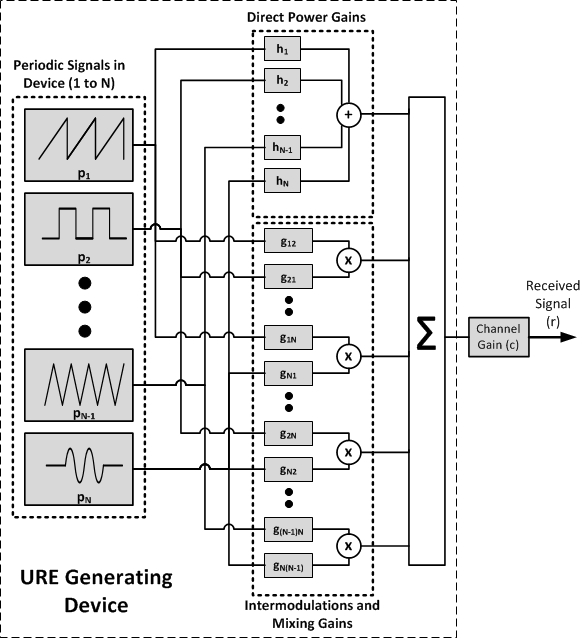
\includegraphics[width=\textwidth]{./model_results/URE_Model.jpg}
	\centering
	\caption{Model of URE generation mechanisms within an electronic device.  URE is composed of the direct conduction components and the intermodulation components of periodic signals utilized within the URE generating device.}
	\label{fig:ure_model}
\end{figure}

The simplified model in Figure \ref{fig:ure_model} does not take in to account the continued mixing and addition of previously multiplied signals which could theoretically continue nearly indefinitely resulting in a significantly increased model complexity.  Given that no assumption was made with regard to the periodic signals ($P_n$), the additional frequency components generated from continued addition and multiplication can be folded in to additional $P$ components or different periodic signal structures. 

\section[Model Development]{Model Development}

Analytically, the received complex URE time domain signal, $r$, can be written as the sum of the direct and intermodulation responses
\begin{equation}
	r ={} c \ast \left(\sum^N_{n=1} p_{n} \ast h_{n} + \sum^N_{i\neq{}j} \left(p_{i} \ast g_{i,j}\right)\left(p_{j} \ast g_{j,i}\right)\right) \label{eq:uremodel1}
\end{equation}
where $r$ is the time domain received signal, $c$ is the URE channel gain, $p_{n}$ are periodic signals used within the devices, $h_{n}$ are the direct power gains for each signal, and $g_{i,j}$ are mixing product gains for component cross-talk and intermodulation, $i$ and $j$ are sequences $1$ to $N$, and $N$ is the number of periodic signals. Note that Equation \ref{eq:uremodel1} assumes no signal mixes with itself.

Using the Convolution Theorem to transform $r$ into its Power Spectral Density (PSD), $\hat{r}$,   
\begin{equation}
    \hat{r} ={} \hat{c} \left( \underbrace{\sum^{N}_{n=1} \hat{p}_{n}\hat{h}_{n}}_\text{Direct Conduction} + \underbrace{\sum^N_{i\neq{}j} \hat{p}_{i}\hat{g}_{i,j} \ast  \hat{p}_{j}\hat{g}_{j,i}}_\text{Mixing Products} \right) \label{eq:uremodel2}
\end{equation}
where $\hat{p}$ is the PSD of $p$ and $\hat{g}$, $\hat{h}$, and $\hat{c}$ are the Fourier transforms of $g$, $h$, and $c$ filter responses, respectively.

Evaluation of the trivial case where $p_1 = \sin(2\pi f_1 t)$, $p_2 = \sin(2\pi f_2 t)$, $c = h_1 = h_2 = g_1 = g_2 = \delta(t)$, and $f_1 \gg f_2$ shows the following 
\begin{equation} \label{eq:uremodelsimpletime}
\begin{split}
	r & = \sin(2\pi f_1 t) + \sin(2\pi f_2 t) + \sin(2\pi f_1 t)\sin(2\pi f_2 t) \\
		& = \sin(2\pi f_1 t) + \sin(2\pi f_2 t) + \frac{1}{2}\cos(2\pi(f_1 - f_2)t) +  \frac{1}{2}\cos(2\pi(f_1 + f_2)t)\\
\end{split}
\end{equation}
which returns the following positive frequency spectral components
\begin{equation} \label{eq:uremodelsimplefreq}
	\hat{r} = \underbrace{\frac{1}{2}\delta(f - f_1) + \frac{1}{2}\delta(f - f_2)}_\text{Unmodulated Frequency Peaks} + \underbrace{\frac{1}{4}\delta\left(f - (f_1 - f_2)\right) + \frac{1}{4}\delta\left(f - (f_1 + f_2)\right)}_\text{Modulation Sidebands}\\
\end{equation}
 
Examination of Equation \ref{eq:uremodelsimplefreq} shows that for the simple case of two periodic signals, two unmodulated frequency tones and two modulation sidebands are present.  The number of potential frequency peaks within a URE spectrum grows at a rate of $\mathcal{O}(n^2)$ for each additional periodic signal and $\mathcal{O}(n^2)$ for each additional harmonic associated with the periodic signals, resulting in combined growth of $\mathcal{O}(n^2) \times \mathcal{O}(n^2) = \mathcal{O}(n^4)$.  For instance, $10$ carriers, with $10$ harmonics each, can generate nearly $10000$ peaks within the frequency domain. The number of potential peaks within the spectrum of a URE signal can be significant, resulting in an overdetermined system with a very large feature space, which DASP is presented to address.   

The continuous-time Fourier Series expansion of a periodic signal shows that it is comprised of an infinite sum of its respective harmonics; therefore, aligning and summing its harmonic content maximizes detection of the signal.  Although the fundamental frequencies of the periodic signals comprising $r$ are unknown, the HASP algorithm provides a method of aligning harmonics of all periodic signals within a given band regardless of the fundamental frequency.  Additionally, the trigonometric product identities show that the intermodulation and mixing of periodic signals results in the sum and differences of the mixing frequencies, as shown in Equation \ref{eq:uremodelsimplefreq}.  The MASP, CMASP, and SCAP algorithms provide a method for detecting these modulations and aligning the frequency mixing sums and differences when the underlying carrier and modulation frequencies are unknown.  As shown in Sections \ref{Harmonically Aligned Signal Projection}, \ref{Modulation Aligned Signal Projection}, \ref{Spectral Correlation Aligned Projection}, \ref{Cross-Modulation Aligned Signal Projection} the HASP, MASP, SCAP, and CMASP algorithms provide a method for aligning and summing harmonics and their cross-products regardless of their underlying fundamental frequency, carrier frequency, and modulation frequency and therefore maximize features relevant to device detection and classification.  Additionally, Section \ref{Frequency Aligned Signal Projection} describes the Frequency Aligned Signal Projection which provides a method for aligning frequencies over time for further characterization of signal harmonic components and their respective time and frequency modulations.

\section[DASP Methodology]{DASP Methodology}

Alignment of signal components, such as harmonics, modulations, and frequencies, with the DASP algorithms result in 2-D images which need to be further processed for extraction of features and eventually used for testing and training in a machine learning framework.   As shown in Figure \ref{fig:dasp_methodology}, raw time domain signal captures are transformed through a DASP process in to a 2-D structure and further processed through an image scaling, segmentation, and summing process.   Statistical features and processed DASP images are then utilized for training and testing using LDA, k-NN, and CNN machine learning processes.  

\begin{figure}[tb]
	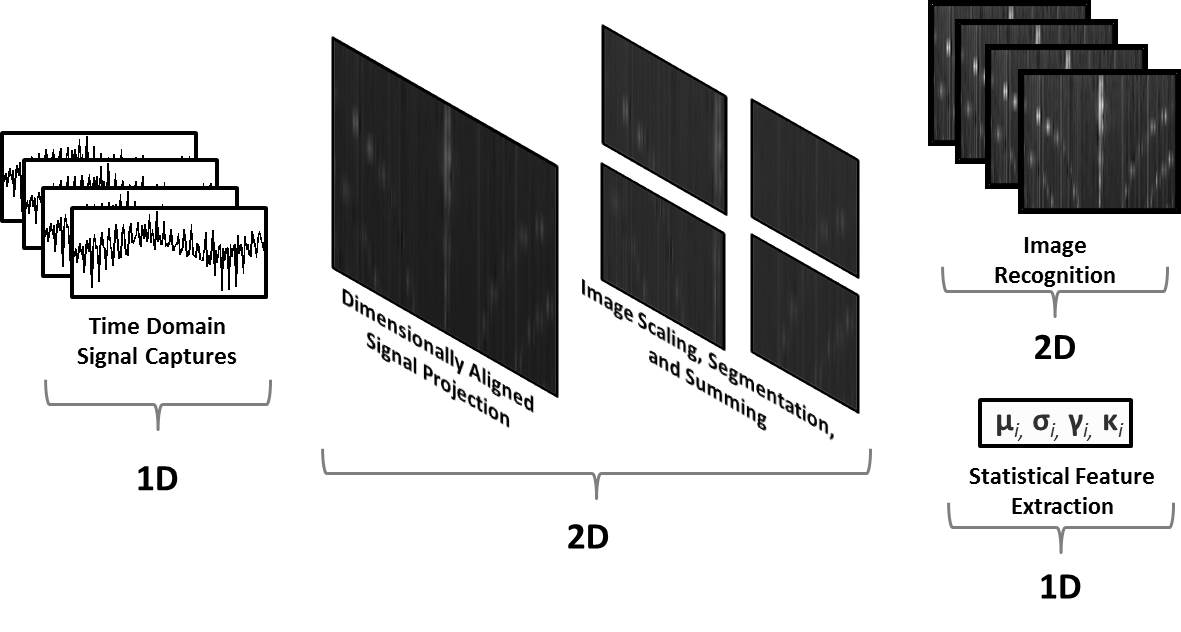
\includegraphics[width=\textwidth]{./model_results/model.jpg}
	\centering
	\caption{DASP processing and feature generation methodology.  The DASP algorithms transform a 1-D vector into a 2-D image which is subsequently transformed, segmented, or processed through an image processing algorithm.  The DASP images are then utilized to classify URE from electrical devices through a variety of feature extraction and learning methods.}
	\label{fig:dasp_methodology}
\end{figure}   
% To compile single chapters put a % symbol in front of "\comment" and "}%end of comment" below 
%    and take off the % symbol from "\end{document" at the bottom line. Undo before compiling
%    the complete thesis
%%Note: You can only use \section command, you are not allowed, per TTU Graduate School, use
%%\subsection command for ghigher level subheadings. At most level 2 subheadings are allowed.

\chapter{URE Data Collection}
\label{URE Data Collection Chapter}

\section[Data Requirements]{Data Set Requirements}

To ascertain the ability of the DASP algorithms and subsequent image processing, feature extraction, and machine learning algorithms to characterize and classify devices based upon their respective URE, a data set of sufficient size and diversity was required to provide reliable statistics and performance metrics.  Table \ref{tab:collection_requirements} outlines the self-imposed URE collection system and device requirements for a data set suitable for evaluation of the DASP algorithms.  No publicly available data sets were identified that met the criteria for evaluation of the DASP algorithms, with the vast majority being too low in sample rate ($< 15$kHz), such as Smart* \cite{Barker2012}, AMPds \cite{Makonin2013}, BLUED \cite{Filip2011}, ECO \cite{Beckel2014}, and iAWE \cite{Batra2014}.  In addition, existing data sets also tended to focus on large appliances or whole house measurements as with the REDD \cite{Kolter2011},  Plaid \cite{Gao2014}, and UK-DALE \cite{Kelly2015}, as opposed to focusing on single measurements of small electronic devices.  \cite{Gulati2014} did provide a high frequency ($>1$Ms/s) data set of EMI signatures from small commercial electronic device, unfortunately the number of data captures per device were not sufficient for the machine learning processing requirements. 

\begin{table}[tb]
	\caption{URE data set collection and device requirements for evaluation of DASP algorithms and their applicability to URE classification.}
	\centering
		\begin{tabular}{c|c}
		\hline
		Metric & Value \\
		\hline
    Sample Rate & $ \ge 1$MS/s\\
		Bits of Resolution & $ \geq 12$ bits \\
		Collection Type & Baseband Measurements Required \\
		Power Line Frequency Filtering & Preferred \\
		Number of Devices & $\geq 10$ Devices \\
		Number of Measurements & $ \geq 100$ per Device\\
		Types of Devices & Consumer Electronic Devices \\
		Measurement of ``Off'' State & Required \\
		Collection Environment & Relatively Low Noise \\
		Ground Truth Documentation & Required \\
		Measurement Type & Ground to Neutral Voltage Preferred \\
		& Ground or Neutral Current Probe Acceptable \\
    \hline
		\end{tabular}
	\label{tab:collection_requirements}
\end{table}

Although many of the constraints in Table \ref{tab:collection_requirements} are self-evident, several were refined through the initial collection and DASP test and evaluation phases.  For instance, early testing showed significant spectral content at frequencies greater than $100$kHz for several devices, as also identified by \cite{Gulati2014}, and therefore a higher sampling rate greater than or equal to $1$MS/s was desired.   In addition, URE content was identified within current probe captures of the ground and neutral lines as well as voltage measurements between the power line conductors, however a voltage probe measurement was preferred given the ease of installation and potential utilization in commercial and residential applications.

\section[Collection Setup]{Collection Setup}

Due to the inability to identify a suitable data set for DASP processing, a collection system was developed and consumer electronic devices gathered to satisfy the requirements set forth in Table \ref{tab:collection_requirements}.  The URE signal captures were performed in a radio frequency (RF) shielded enclosure using a Universal Software Radio Peripheral (USRP) N210 collection platform with an LFRX analog-to-digital processing board operating at $2$MS/s.  The conducted URE signals were measured using a high impedance differential voltage probe between the ground and neutral conductors providing power to the RF chamber, as pictured in Figure \ref{fig:chamber_pic}.  A Twin-T high-pass filter \cite{Cooke2016} was installed in series with the high impedance voltage probe, as shown in Figure \ref{fig:twint_filter_schematic}, to reduce the $60$Hz power line frequency and maximize the dynamic range of the system.  The voltage attenuation response versus frequency is shown in Figure \ref{fig:twint_filter_response}.

\begin{figure}[tb]
	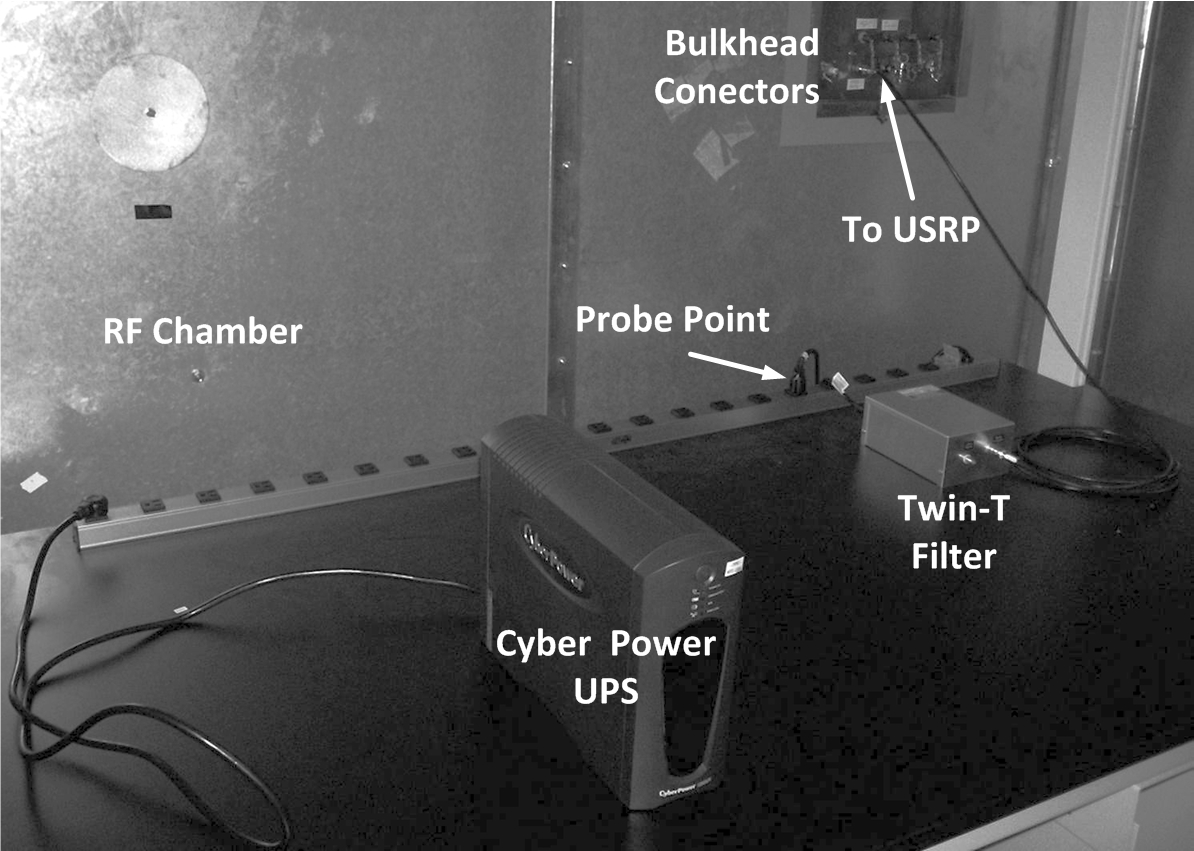
\includegraphics[width=\textwidth]{./data_collection_results/chamberAdj.jpg}
	\centering
	\caption{Picture of URE signal collection being performed on the \textit{cyberpowerups} device.  URE collection was conducted within an RF shielded enclosure with the filtered differential probe signal relayed to an external collection system through an RF bulkhead connection.}
	\label{fig:chamber_pic}
\end{figure}

\begin{figure}[tb]
	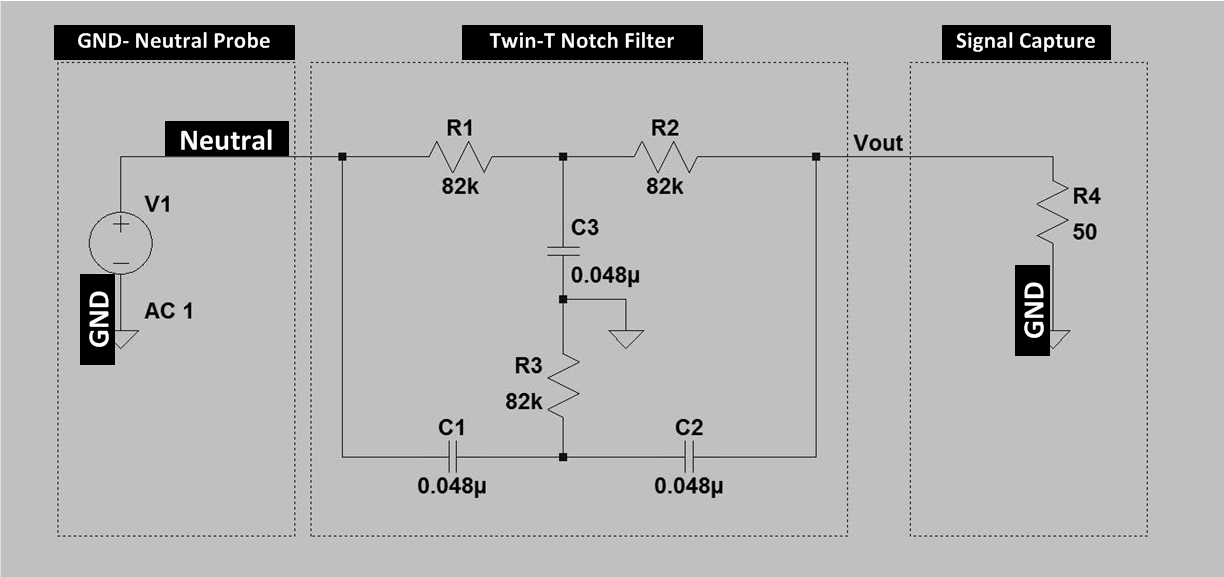
\includegraphics[width=\textwidth]{./data_collection_results/filter_schematic}
	\centering
	\caption{Schematic of Twin-T notch filter used for filtering the $60$Hz power line frequency.  The conducted URE signal sampling was performed with a differential measurement between the power line neutral and ground, with sampling performed by a USRP N210.}
	\label{fig:twint_filter_schematic}
\end{figure}

\begin{figure}[tb]
	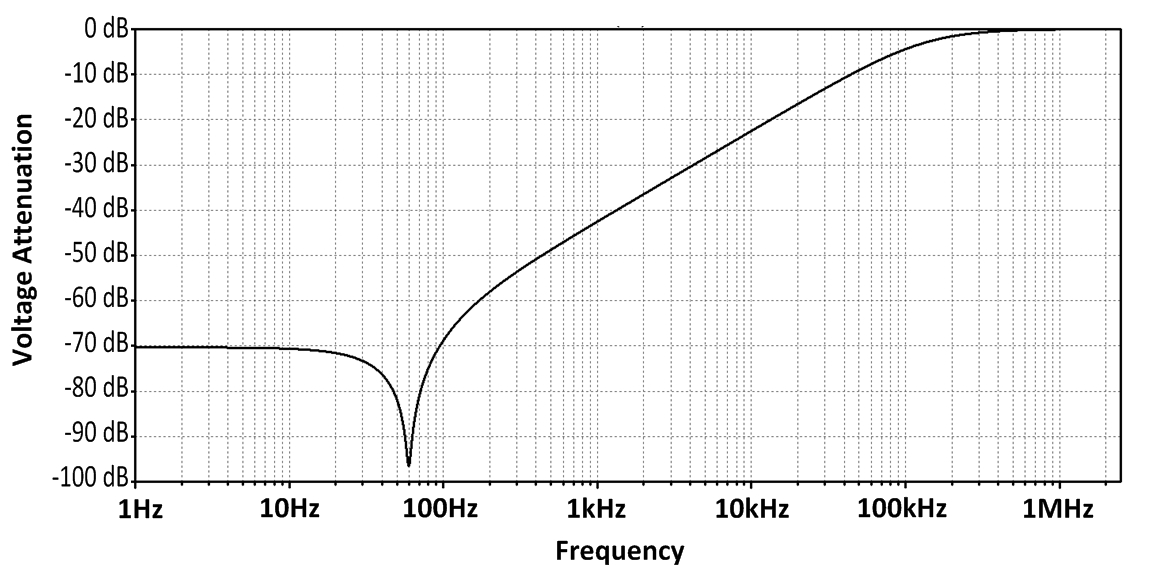
\includegraphics[width=\textwidth]{./data_collection_results/filter_response.jpg}
	\centering
	\caption{Twin-T voltage attenuation response versus frequency.  The filter was designed to provide a greater than $50$dB voltage attenuation to the power line frequency and its first harmonic ($60$Hz and $120$Hz) \cite{Cooke2016}.}
	\label{fig:twint_filter_response}
\end{figure}

The USRP N210 was equipped with a temperature-compensated crystal oscillator (TCXO) which provided a $2.5$ parts-per-million (ppm) frequency accuracy.  Although the TCXO did not provide the temperature stability of oven-controlled or GPS disciplined oscillators, the lower cost, size, and power requirements of the TCXO provided a viable basis for low cost commercial applications.  To further demonstrate commercial applicability, no effort was made to calibrate or quantify the frequency stability of the USRP N210 collection system.

\section[Test Devices]{Test Devices}

Twenty-one commercially available consumer electronic devices were selected for URE collection in the RF shielded enclosure.  The devices were selected to represent a typical home and office environment, with class types ranging from computing platforms to gaming systems to media players.  The devices, along with the inclusion of the \textit{None} state, were separated in to two data sets to represent ``known'' devices for ``Testing and Training'' and ``Unknown'' devices for ``Clutter'' analysis as shown in Table \ref{tab:collection_devices}, where the class names and class descriptions are provided for each device.  Pictures of the ``Test and Training'' devices are shown in Figure \ref{fig:device_pics} as they were positioned in the RF enclosure during the URE collection process.

\begin{table}[tb]
	\caption{A listing of all of the commercial devices utilized for the collection of conducted URE.  Devices were divided between ``Test and Training'' and ``	Clutter''.  In addition to the ``None'' class, the ``Test and Training'' devices were utilized for the majority of analysis, whereas the ``Clutter'' devices were used for clutter analysis as presented in Chapter \ref{DASP Device Classification Chapter}.}
	\centering
		\begin{tabular}{cc|cc}
		\hline
		\multicolumn{2}{c}{Test and Training Devices} & \multicolumn{2}{c}{Clutter Devices} \\
		Description & Name & Description & Name\\
		\hline
    None & None & BluRay Player & viziobluray \\
		UPS & cyberpowerups & Desk Phone & cortelphone \\
		Monitor & dellmonitor & Desk Phone & lgphone \\
		Desktop & delloptiplex & Single Board Computer & odroidxu4 \\
		Desktop & dellxps & VOIP Phone & polycomvoip \\
		Light & fluorescentlights & Single Board Computer & raspberrypi \\
		Printer & hplaserjet & Media Player & roku2xs \\
		Laptop & hpzbook & Single Board Computer & usrpe310 \\
		Router & linksysrouter & Gaming System & vtechvsmile \\
		Monitor & viewsonicmonitor & Gaming System & wiiu\\
		& & Gaming System & xboxone\\
    \hline
		\end{tabular}

	\label{tab:collection_devices}
\end{table}

\begin{figure}[tb]
	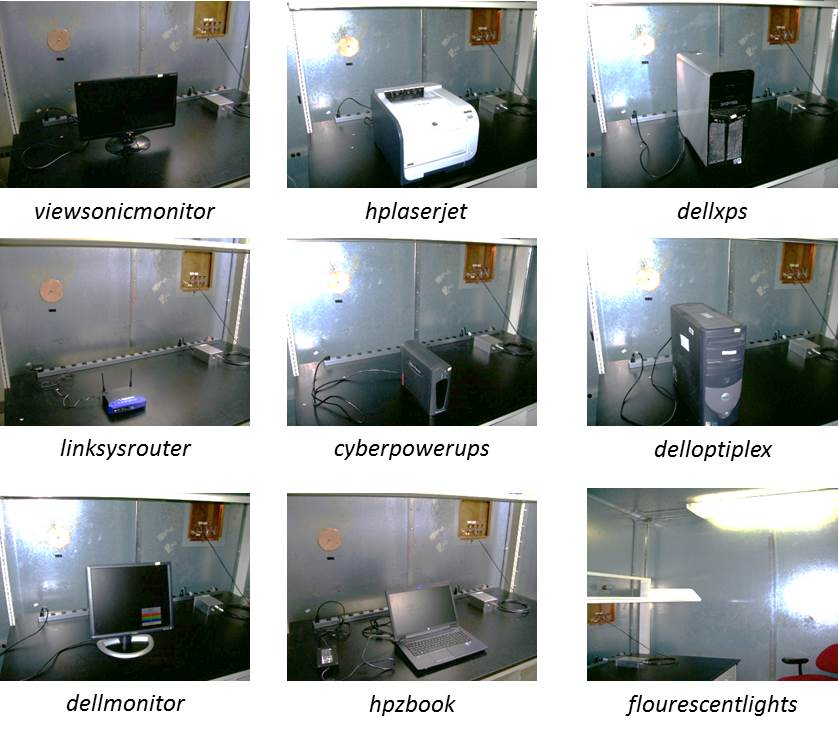
\includegraphics[width=\textwidth]{./data_collection_results/device_pics.jpg}
	\centering
	\caption{Testing and training devices shown in the RF enclosure before collection of URE was conducted.}
	\label{fig:device_pics}
\end{figure}

\section[Collection Process]{Collection Process}

To minimize the noise and confounders in the URE data sets, the devices of interest were placed in an RF shielded enclosure with a power line filtering system.  The collection system was placed outside of the RF shielded enclosure while being fed via a bulkhead connection to the voltage probe within the enclosure.  During collection periods, all electrical devices within the enclosure were powered down except for the device under test.  A set of fluorescent lights was installed in the enclosure and were also turned off during collection periods, except during collection of the \textit{fluorescentlights} device class.  

Collection periods were divided into four $10$ minute segments with the device turned on for the first and third segments and the device unplugged for the second and fourth segments.  Each $10$ minute time domain capture was subsequently divided into contiguous one second capture files resulting in a total of $1200$ time domain captures per device and  $24000$ ``off state'' captures, with each one second time domain capture stored in a MATLAB\textsuperscript \textregistered ~ \textit{.mat} file structure with the fields shown in Table \ref{tab:collection_parameters}.  To allow for software boot-up time and to ensure steady-state operation, a minimum wait period of one minute was provided after the devices were powered on and before signal captures were started.  Additionally, no specific process for exercising the devices under test was conducted, such as playing a Blu-Ray disk or running a specific software application, and furthermore, no provisions were made to prevent a device from entering a low-power or sleep mode during the $10$ minute collection windows.

\begin{table}[tb]
	\caption{Table of recorded fields for each URE collection sample.  In addition to the raw data (\textit{data}), the collection conditions, device information, and collection time are all recorded.}
	\centering
		\begin{tabular}{c|c|c}
		\hline
		Field Name & Description & Example \\
		\hline
    \textit{data} & Time domain sampled signal & $1 \times 200000$ int16 vector \\
		\textit{samp\_rate} & Sample Rate & $2000000$ \\
		\textit{meastype} & Voltage probe configuration & \textit{ng} (i.e Neutral to Ground) \\
		\textit{devclass} & Class of Device & \textit{phone} \\
		\textit{devname} & Name of Device & \textit{cortelphone} \\
		\textit{partnum} & Part Number of Device & \textit{270000 TP2 27S} \\
		\textit{serialnum} & Serial Number of Device & \textit{027046} \\
		\textit{year} & Collection Year & $2016$ \\
		\textit{month} & Collection Month & $6$ \\
		\textit{day} & Collection Day & $24$ \\
		\textit{hour} & Collection Hour & $16$ \\
		\textit{minute} & Collection Minute & $5$ \\
		\textit{second} & Collection Second & $6$ \\
    \hline
		\end{tabular}
	\label{tab:collection_parameters}
\end{table}    
% To compile single chapters put a % symbol in front of "\comment" and "}%end of comment" below 
%    and take off the % symbol from "\end{document" at the bottom line. Undo before compiling
%    the complete thesis
%%Note: You can only use \section command, you are not allowed, per TTU Graduate School, use
%%\subsection command for ghigher level subheadings. At most level 2 subheadings are allowed.

\chapter{DASP Algorithm Development}
\label{DASP Algorithm Development Chapter}

\section[DASP Overview]{DASP Overview}

The processing of conducted URE for the purposes of device classification often requires intimate knowledge of the underlying signal characteristics which are determined by the physical implementation of the device's electronic circuitry.  DASP provides a method for aligning those signal dimensions inherent to the majority of electronic circuits without prior knowledge of the device's physical or conducted noise characteristics.  The following DASP algorithms are presented to align conducted URE dimensions of interest for device classification: Harmonically Aligned Signal Projection (HASP), Modulation Aligned Signal Projection (MASP), Cross-Modulation Aligned Signal Projection (CMASP), and Spectral Correlation Aligned Projections (SCAP).   In addition, two different methods for implementing the HASP algorithm will be presented, the fixed and decimating types.

An additional DASP algorithm widely used within the signal processing community is the Short-Time Fourier Transform (STFT, sometimes referred to as a spectrogram) \cite{Welch1967, Allen1977, Griffin1984}.  The STFT computes the Fast Fourier Transforms (FFT) over short time segments and \textit{aligns} the frequency bins of these FFT segments over time.  For consistency, I will use the term Frequency Aligned Signal Projection (FASP) for the STFT when used in the context of a DASP transform.   

Techniques for processing and extracting features from DASP output arrays are discussed in Chapter \ref{DASP Feature Extraction Chapter}.  Chapter \ref{DASP Device Classification Chapter} provides results from the application of supervised and unsupervised machine learning techniques to DASP generated arrays and features to determine the applicability of dimensional alignments to classify devices based upon their URE.

\section[Harmonically Aligned Signal Projection (HASP)]{Harmonically Aligned Signal Projection}
\label{Harmonically Aligned Signal Projection}

The HASP algorithm provides a method for aligning a fundamental frequency with its respective harmonics in the column of a 2D matrix.   Harmonic content analysis can provide information related to a signal's stability, shape, and the underlying physical circuitry.  All non-pure sinusoidal periodic functions, such as square or triangle waves, are composed of harmonics with varying magnitudes and phases which define the shape of the time domain signal.  Aligning the harmonic structure of a signal is complicated by frequency uncertainties and offsets of the underlying fundamental.  For instance, the $40$th harmonic of a $50$Hz signal should be at $2000$Hz exactly, however a $0.5$Hz offset in the fundamental will result in the $40$th harmonic appearing at $2020$Hz.  Assuming a $1$Hz frequency resolution in the FFT, the harmonic will appear $20$ bins from where expected. To demonstrate, Figure \ref{fig:harm_aligned_example} shows the alignment of frequency bins through the $40$th harmonic for an exact $50$Hz signal and one with a $0.5$Hz offset. 

\begin{figure}[tb]
	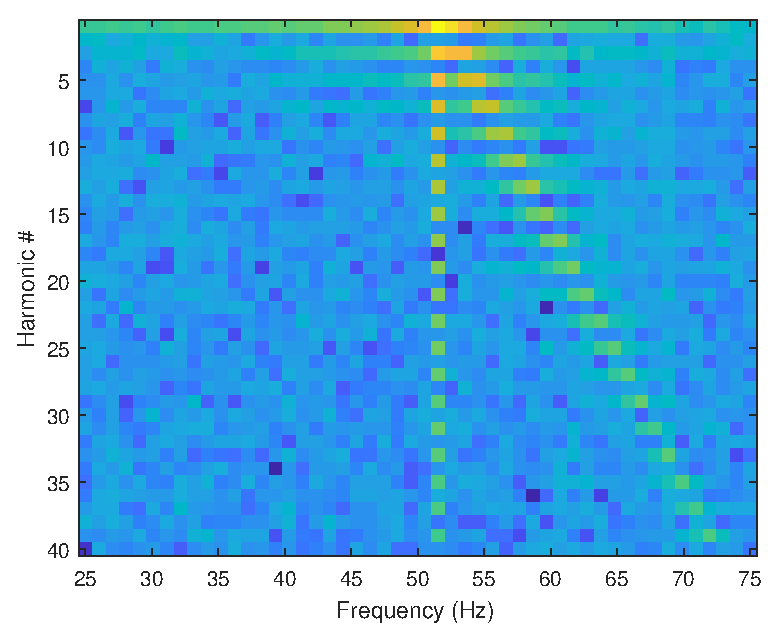
\includegraphics[width=\textwidth]{./dasp_algorithm_results/harmonic_aligned_example.eps}
	\centering
	\caption{Image showing the alignment of the harmonics of $50$Hz and $50.5$Hz square waves from a synthetic test signal generated from the addition of two square waves with $50$Hz and $50.5$Hz fundamental frequencies.  The frequency of each row is multiplied by the harmonic number, such that the center bin of the second row is $2 \times 50$Hz$ = 100$Hz.  The last row shows the $40$th harmonic of the $50$Hz signal at $2000$Hz and the $40$th harmonic of the $50.5$Hz signal at $2020$Hz.}
	\label{fig:harm_aligned_example}
\end{figure}

In addition to the misalignment of the $50.5$Hz fundamental with its respective harmonics, the harmonic structure of a square wave is evidenced by the alternating intensities of harmonics.  Every odd harmonic row (i.e. $3$rd, $5$th, $7$th, etc.) shows a harmonic signal, whereas the even harmonic rows ($2$nd, $4$th, $6$th, etc.) do not appear to show any harmonic structure.

\subsection[Harmonically Aligned Signal Projection - Fixed Type (HASP-F)]{Harmonically Aligned Signal Projection - Fixed Type (HASP-F)}
\label{Harmonically Aligned Signal Projection - Fixed Type}

Figure \ref{fig:harm_aligned_example} provides an example of the Fixed Type HASP algorithm (HASP-F), where a fixed number of frequency bins are selected around a specific fundamental and its respective harmonics and are aligned in to rows to form a 2-D image.  Assuming the fundamental frequency is known perfectly, the harmonics will align within a single column and provide a strong feature that could be used for classification purposes, as shown in the diagram of the HASP-F process in Figure \ref{fig:haspf_diagram_independent}.  In addition, modulation sidebands centered around the fundamental frequency and its harmonics also align within the HASP-F image, as shown in Figure \ref{fig:haspf_diagram_modulation}, and provide an additional dimension alignment and further insights in to the underlying signal structure.

\begin{figure}[tb]
	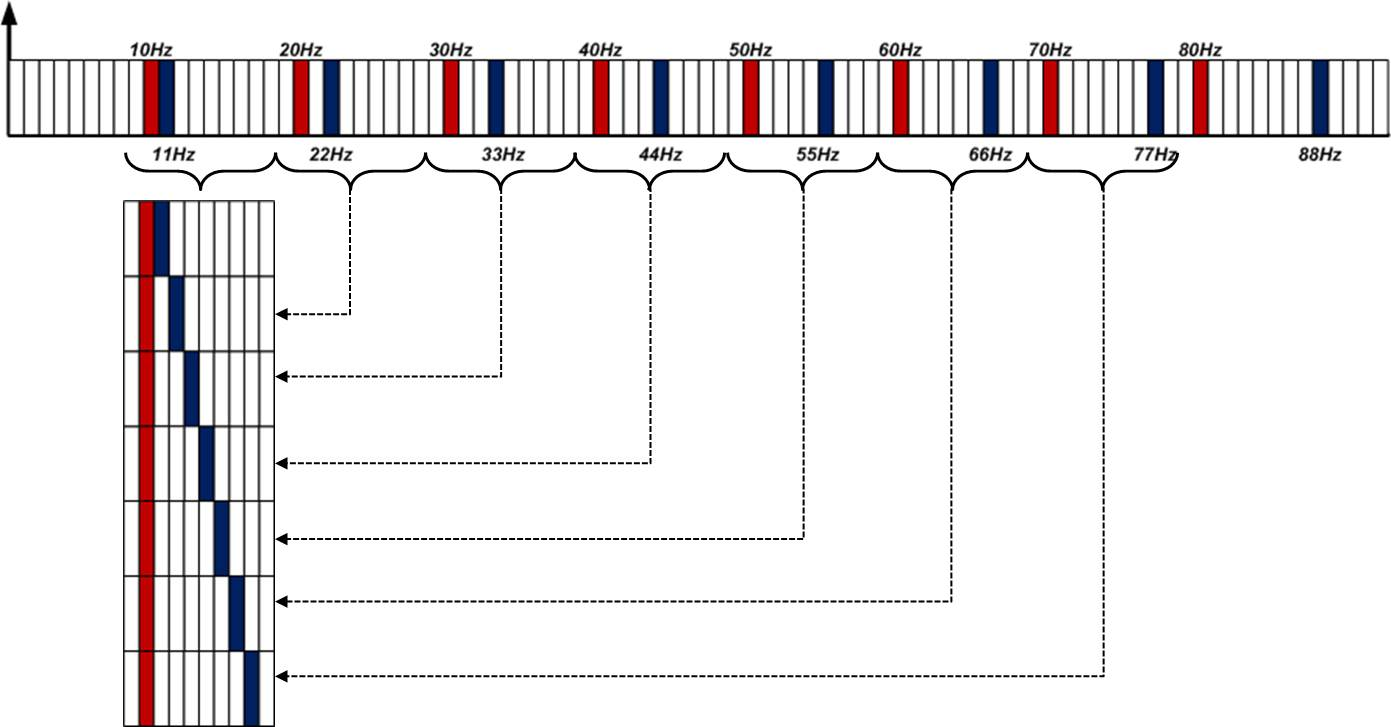
\includegraphics[width=\textwidth]{./misc_graphics/haspf_diagram_independent.jpg}
	\centering
	\caption{Diagram of the HASP-F process applied to two independent carriers at $10$Hz and $11$Hz with harmonic content, as represented by the red and blue blocks, respectively, and each frequency bin represents a $1$Hz resolution.  As a fixed number of bins are selected to align the $10$Hz harmonics, the $11$Hz harmonics slant across the image.}
	\label{fig:haspf_diagram_independent}
\end{figure}

\begin{figure}[tb]
	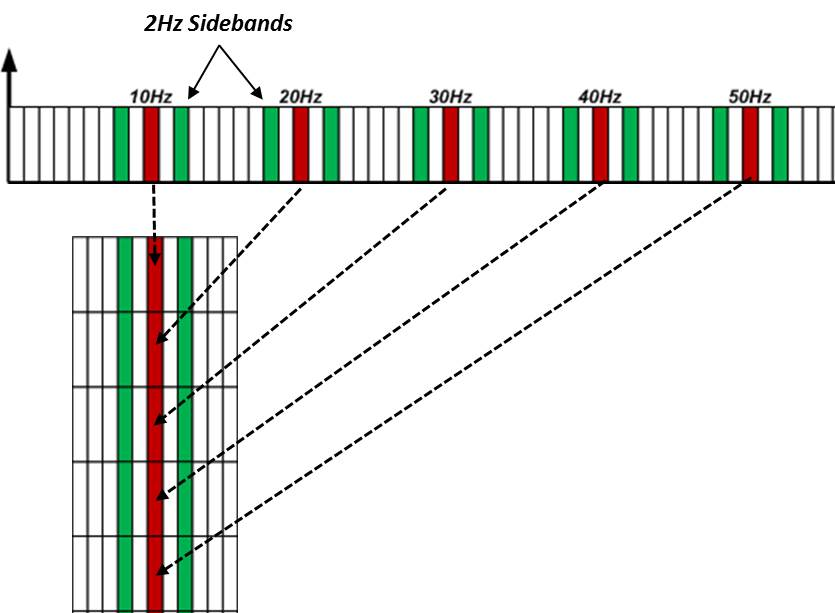
\includegraphics[width=\textwidth]{./misc_graphics/haspf_diagram_modulation.jpg}
	\centering
	\caption{Diagram of the HASP-F process applied to a carrier at $10$Hz with $2$Hz modulation sidebands, as represented by the red and green blocks, respectively.  As a fixed number of bins are selected to align the $10$Hz harmonics, the $2$Hz sidebands also align accordingly.}
	\label{fig:haspf_diagram_modulation}
\end{figure}

As demonstrated in Figure \ref{fig:haspf_diagram_independent}, the $10$Hz fundamental frequency aligns with its respective harmonics when a fixed number of frequency bins are selected around each harmonic, whereas, the $11$Hz independent carrier slants across the 2-D array because each progressive $11$Hz harmonic is $1$Hz, or $1$ frequency bin, further away from the corresponding $10$Hz harmonic.  Because modulation sidebands are always at fixed frequencies around both the fundamental and its harmonics, Figure \ref{fig:haspf_diagram_modulation} shows that modulation sidebands also align when performing fixed harmonic alignment. 

As evidenced from Figure \ref{fig:haspf_diagram_independent} and Figure \ref{fig:haspf_diagram_modulation}, the fixed harmonic alignment requires a specific fundamental frequency to be known and selected for perfect vertical alignment to occur, otherwise any frequency offset will result in a slanted line in the resulting 2-D image.  The HASP-F algorithm is described in more detail in Algorithm \ref{alg:haspfalg}. The algorithm operates on a frequency domain input, $\hat{r}$, along with the input parameters $f_c$ and $B$, center frequency and bandwidth, respectively. The final 2D image will be a function of $f_c$, the center frequency of the image, and $B$, the bandwidth around this center frequency (or width of the image). The algorithm first derives the maximum harmonic, $K$, of $f_c$, based on the sampling frequency and the bandwidth around $f_c$.  The maximum harmonic, $K$, corresponds to the height of the 2-D HASP image, where each row of the image corresponds to the $k$th harmonic of $f_c$. The image is formed by iterating through all harmonics from the fundamental frequency to the maximum harmonic $K$.  For each harmonic, the magnitude of the input PSD, $\hat{r}$, is indexed by the corresponding $(k \times f_c) \pm B$ frequency bins, where $k$ is the harmonic number $\left[1,2,3 \ldots{} K \right]$.  Each row is comprised of a fixed number of frequency bins as set by the bandwidth, $B$, around the fundamental frequency.  The resulting HASP-F image dimensions are $K$ by the number of discrete frequency bins comprising the continuous frequencies $f_c \pm B$. 
 
\begin{algorithm}
	\caption{Harmonic Aligned Signal Projection Algorithm - Fixed Type (HASP-F)} \label{alg:haspfalg}
	\scriptsize
	\centering
	\begin{algorithmic}[1]
		\Require~~
		\Statex $\hat{r}$ - Input Power Spectrum
		\Statex $f_c$ - Center Frequency 
		\Statex $B$ - Bandwidth
		\Ensure~~
		\Statex $\bf{H}$ - HASP Output Array
		\Statex
		\For  {$k = 1, 2, \ldots K$} 
		\State    $\mathbf{f}_k \gets \left[ \hat{r}(x_i) \right], (k \times f_c) - B \leq x_i \leq (k \times f_c) + B$
		\State		$k$-th row of $\mathbf{H} \gets \mathbf{f}_k$
		\EndFor
	\end{algorithmic}
\end{algorithm}

To illustrate the HASP-F algorithm images, conducted URE was collected from fluorescent lights in an RF shielded enclosure using a USRP N210 collection platform with an LFRX analog to digital processing board operating at $2$MS/s, as described in Chapter \ref{URE Data Collection Chapter}.  Figure \ref{fig:hasp_fft_example} is a plot of the FFT of the conducted URE collected from two fluorescent light fixtures, showing a fundamental frequency at approximately $45$kHz along with $21$ harmonics up to $1$MHz.  Figure \ref{fig:haspf_example} is the resulting image after application of the HASP-F algorithm to the frequency spectrum of the same time-domain capture.  The blurred vertical line and additional blurred slanting line represent the harmonic structure of the two different fluorescent lights with a very minute frequency difference between their respective crystal oscillators.  The center frequency, $f_c$, of the HASP-F image was selected to vertically align one of the oscillators resulting in a progressively increasing offset for each harmonic of the second crystal oscillator.  

\begin{figure}[tp]
	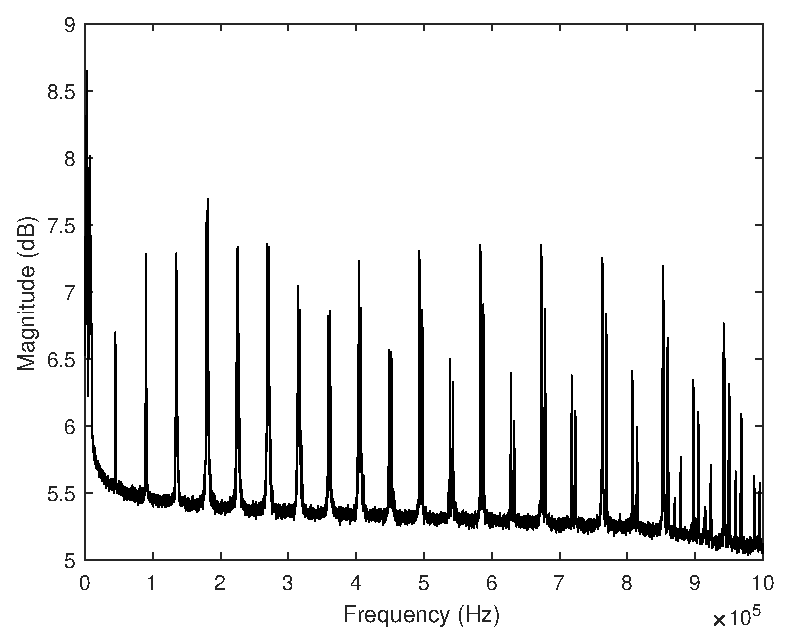
\includegraphics[width=\textwidth]{./dasp_algorithm_results/hasp_fft_filenum_9601.eps}
	\centering
	\caption{Plot of an FFT derived from a time domain capture of conducted URE from a set of fluorescent lights.  The lights have a dominant URE signal with an approximate $45$kHz fundamental frequency.  The plot shows the slight separation of the URE from the two lights at higher frequencies due to the minor differences in the electronic ballasts used within the different lights.}
	\label{fig:hasp_fft_example}
\end{figure}

\begin{figure}[tp]
	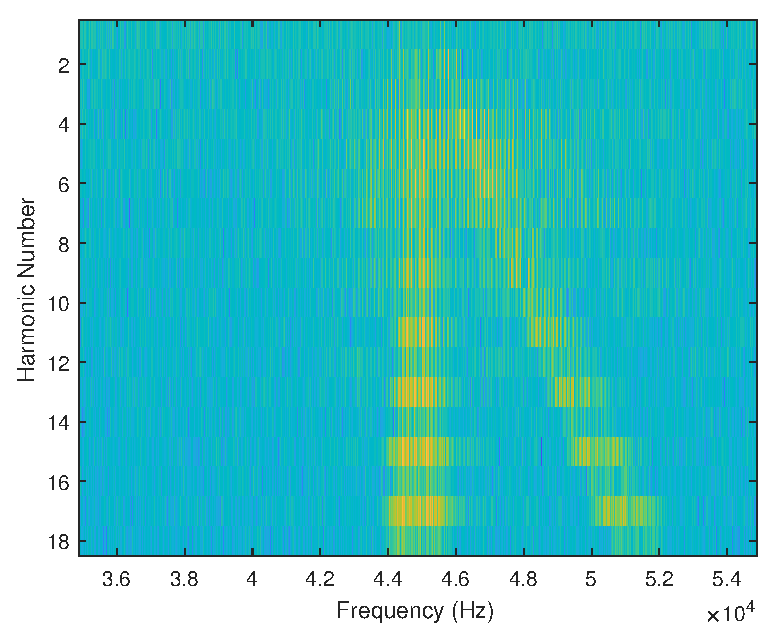
\includegraphics[width=\textwidth]{./dasp_algorithm_results/hasp_f_wide_filenum_9601.eps}
	\centering
	\caption{HASP-F output of the frequency domain signal shown in \ref{fig:hasp_fft_example}.  The separation of harmonics at higher frequencies for the two electronic ballasts can be seen, however the two harmonic alignments are blurred which further demonstrate a low level modulation or instability in the fundamental frequency of the URE generators.}
	\label{fig:haspf_example}
\end{figure}

Analysis of Figure \ref{fig:haspf_example} shows that the two URE generators were roughly $7$kHz apart at the $18$th harmonic.  The frequency offset between the oscillators in the two fluorescent lights was then approximated to be $390$Hz by $7$kHz $/18 \approx 390$Hz.  

\subsection[Harmonically Aligned Signal Projection - Decimation Type (HASP-D)]{Harmonically Aligned Signal Projection - Decimation Type (HASP-D)}
\label{Harmonically Aligned Signal Projection - Decimation Type}

Although the HASP-F algorithm provides a method for aligning harmonics and modulation sidebands, the fundamental frequency needs to be known precisely or the fundamental frequency harmonics will not vertically align and, in addition, the harmonic structures of independent carriers within the HASP-F image will form a slanted line.  The HASP Decimation type (HASP-D) algorithm was developed to vertically align the harmonics of independent signals regardless of the chosen center frequency or amount of frequency offset between the carriers.  The HASP-D algorithm is illustrated in Figure \ref{fig:haspd_diagram_independent}, where each progressive harmonic row is decimated to a fixed number of bins to realign independent harmonics.  Although independent carriers and their respective harmonics align vertically, modulation sidebands ``curve'' in toward the aligned harmonics as the bandwidth around the fundamental is collapsed in to fewer and fewer bins through the decimation process, as shown in Figure \ref{fig:haspd_diagram_modulation}.

\begin{figure}[tp]
	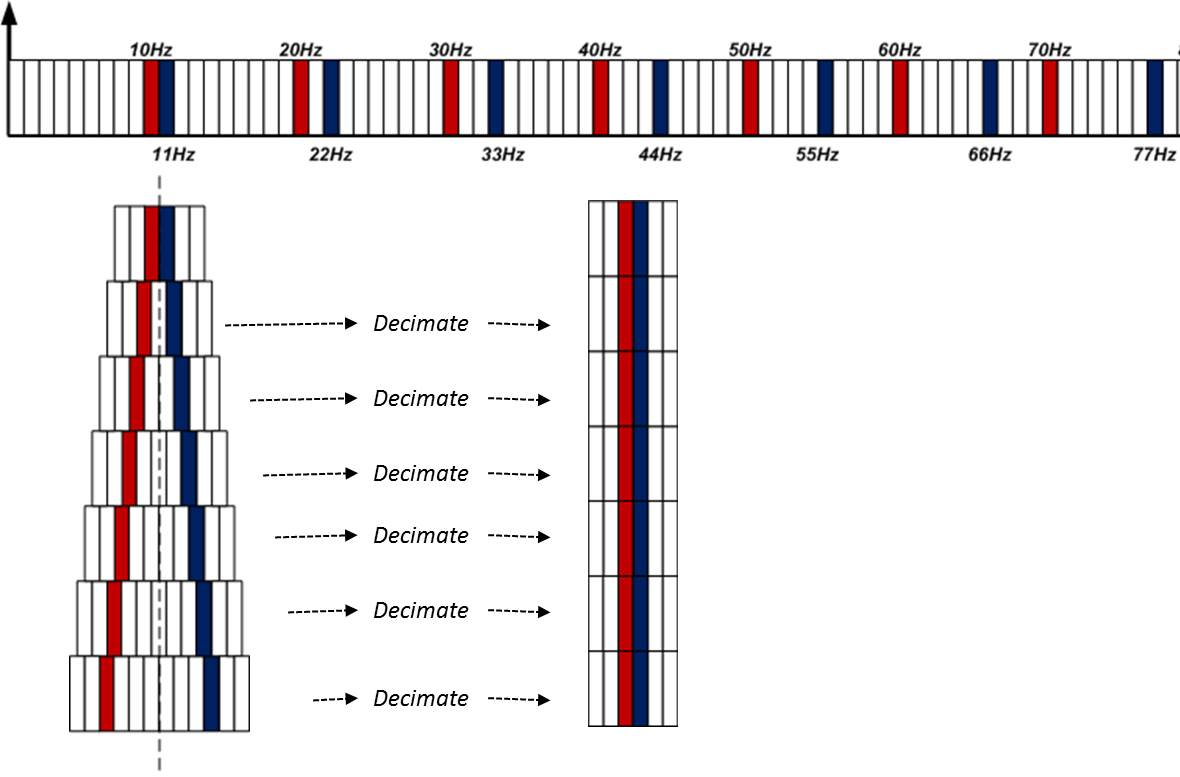
\includegraphics[width=\textwidth]{./misc_graphics/haspd_diagram_independent.jpg}
	\centering
	\caption{Diagram of the HASP-D process applied to a two independent carriers at $10$Hz and $11$Hz with harmonic content, as represented by the red and blue blocks, respectively.  As each harmonic row is added, the number of bins is decimated to equal the number of bins around the fundamental, thus aligning the independent carriers.}
	\label{fig:haspd_diagram_independent}
\end{figure}

\begin{figure}[tp]
	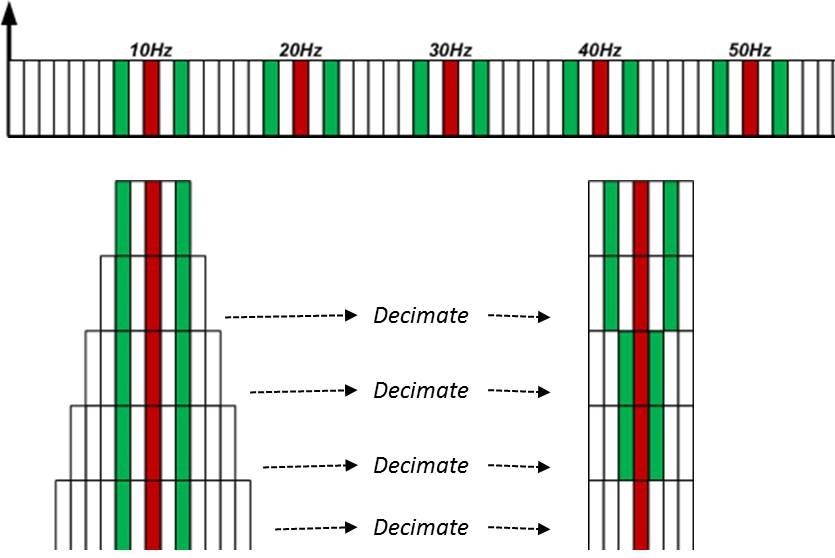
\includegraphics[width=\textwidth]{./misc_graphics/haspd_diagram_modulation.jpg}
	\centering
	\caption{Diagram of the HASP-D process applied to a carrier at $10$Hz with $2$Hz modulation sidebands, as represented by the red and green blocks, respectively.  As each harmonic row is added, the number of bins is decimated to equal the number of bins around the fundamental, thus causing the modulation sidebands to curve in to eventually add with the carrier frequency harmonics.}
	\label{fig:haspd_diagram_modulation}
\end{figure}

As shown in Figure \ref{fig:haspd_diagram_independent}, the number of bins selected around the fundamental frequency determines the resulting number of bins for each harmonic row.   With each progressive harmonic, the number of indexed bins expands by the harmonic number and is then subsequently decimated by the corresponding harmonic number resulting in a vector of bins corresponding to the number of bins in the fundamental frequency row.   By collapsing each row through the decimation process, independent carriers align with their respective harmonics, whereas modulation sidebands that are a fixed number of bins around a given harmonic are ``squeezed'' in toward their respective carrier frequency.   

The HASP-D algorithm is described in more detail in Algorithm \ref{alg:haspdalg} and only differs slightly from the HASP-F algorithm. Identical to the HASP-F algorithm, the HASP-D algorithm operates on a frequency domain input, $\hat{r}$, and requires center frequency and bandwidth input parameters, $f_c$ and $B$, respectively.  The algorithm derives the maximum harmonic, $K$, of $f_c$, based on the sampling frequency and the bandwidth around $f_c$. The maximum harmonic, $K$, corresponds to the height of the 2-D HASP image, where each row of the image corresponds to the $k$th harmonic of $f_c$. The image itself is created by iterating through all harmonics from the fundamental frequency to the maximum harmonic $K$.  For each harmonic, the $\hat{r}$ vector is indexed by the corresponding $k(f_c \pm B)$ frequency bins, where $k$ is the harmonic number $\left[1,2,3 \ldots{} K \right]$.  Because of the expansion of each harmonic vector at increasing $k$, each vector is downsampled by a factor of $k$ to align harmonically related bins in the HASP-D image.  The resulting HASP-D image dimensions are $K$ by the number of discrete frequency bins comprising the continuous frequencies $f_c \pm B$, which are the same dimensions as the HASP-F image.

\begin{algorithm}
	\caption{Harmonic Aligned Signal Projection Algorithm - Decimation Type (HASP-D)} \label{alg:haspdalg}
	\scriptsize
	\begin{algorithmic}[1]
		\Require~~
		\Statex $\hat{r}$ - Input Power Spectrum
		\Statex $f_c$ - Center Frequency 
		\Statex $B$ - Bandwidth
		\Ensure~~
		\Statex $\bf{H}$ - HASP-D Output Array
		\Statex
		\For  {$k = 1, 2, \ldots K$} 
		\State    $\mathbf{f}_k \gets \left[ \hat{r}(x_i) \right], k(f_c - B) \leq x_i \leq k(f_c + B)$
		\State		$k$-th row of $\mathbf{H} \gets$ DOWNSAMPLE $\mathbf{f}_k$ by factor of $k$
		\EndFor
	\end{algorithmic}
\end{algorithm}

To further analyze the URE signal processed by the HASP-F algorithm in Figure \ref{fig:haspf_example}, the HASP-D algorithm was applied to the same frequency domain signal, as shown in Figure \ref{fig:haspd_example}.  The HASP-D image demonstrates the alignment of independent fundamental frequencies and their respective harmonics.  The two vertical lines centered around $45$kHz represent the two independent oscillator signals previously identified in Figure \ref{fig:hasp_fft_example} and Figure \ref{fig:haspf_example}.  The frequency offset between the two oscillators was found to be approximately $300$Hz through visual inspection which roughly corresponds to the calculations derived from the HASP-F image in Figure \ref{fig:haspf_example}.

\begin{figure}[tp]
	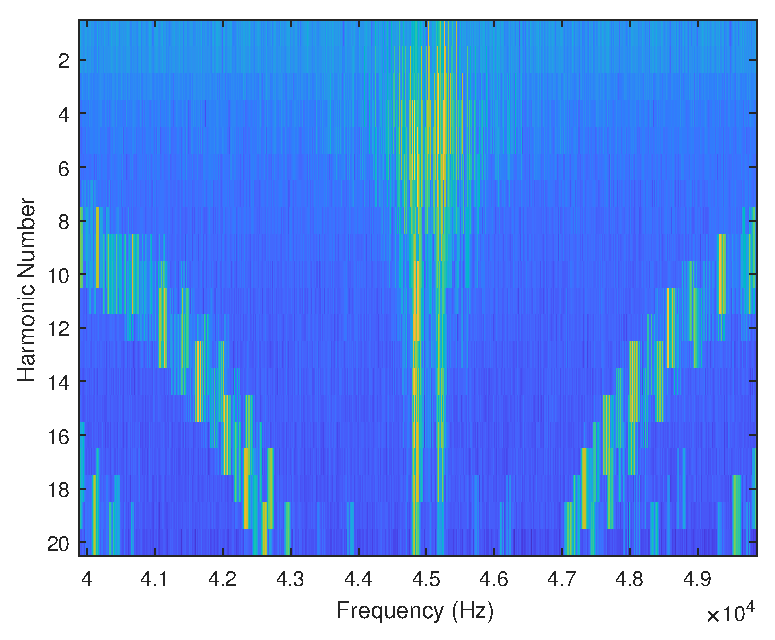
\includegraphics[width=\textwidth]{./dasp_algorithm_results/hasp_d_filenum_9601.eps}
	\centering
	\caption{HASP-D output of the frequency domain signal shown in Figure \ref{fig:hasp_fft_example}.  The HASP-D algorithm decimates each progressive harmonic row to realign harmonic frequency bins to the fundamental frequency row (i.e. row number $1$).  The two independent URE generator signals are now fully parallel because their respective harmonics are aligned across each harmonic row through the decimation process.}
	\label{fig:haspd_example}
\end{figure}

The curved lines centered on the independent carriers in Figure \ref{fig:haspd_example} are artifacts of the preceding and following carrier harmonics due to the expansion and subsequent decimation of each increasing harmonic row.  This was verified by calculating the frequency difference between the curved lines and the harmonic frequency at the $20$th harmonic row, $20 \times (44.8 - 42.6)$kHz $\approx 45$kHz, which corresponds to the fundamental frequency as well as the frequency spacing between all harmonics.

As previously noted in Figure \ref{fig:haspf_example}, the HASP-F image shows a blurring of the two independent carriers which were examined further by applying the HASP-D algorithm with a smaller bandwidth as shown in Figure \ref{fig:haspd_example_zoom}. The blurring, or instability, in Figure \ref{fig:haspf_example} appeared to be the result of a moderate oscillator instability and a low level modulation of the URE generator carrier frequency, as illustrated by the width of the center aligned harmonics and the curved modulation lines, respectively.  

\begin{figure}[tp]
	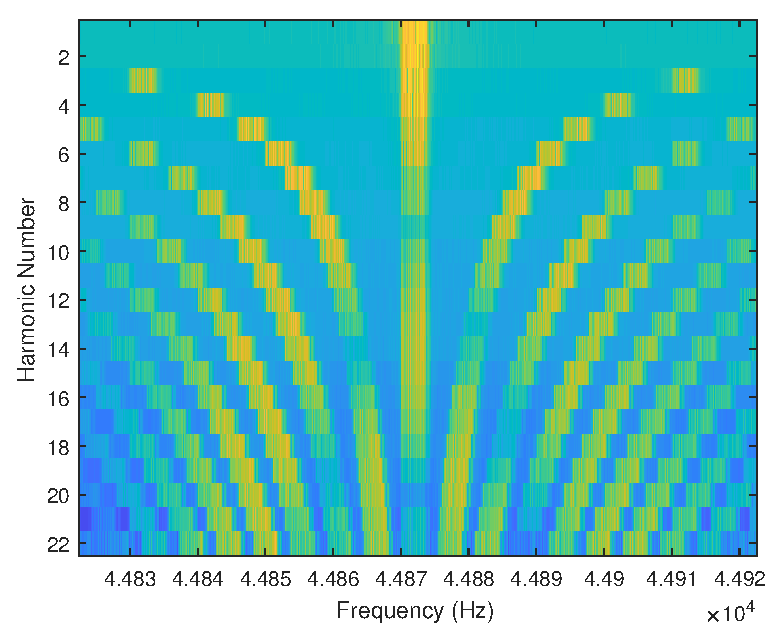
\includegraphics[width=\textwidth]{./dasp_algorithm_results/hasp_d_zoom_filenum_9601.eps}
	\centering
	\caption{Zoomed in view of the HASP-D output of the frequency domain signal shown in Figure \ref{fig:hasp_fft_example}.  The blurring was found to be approximately $4$Hz wide resulting in roughly $\pm 45$ppm carrier stability.  The curved lines centered around the carrier frequency were due to $120$Hz modulations of the carrier frequency.}
	\label{fig:haspd_example_zoom}
\end{figure}

The oscillator instability was found to be approximately $4$Hz wide, corresponding to an approximate clock stability of $\pm 45$ppm, which is consistent with typical inexpensive crystal oscillators.  The sideband peak frequency offsets were found to be approximately $120$Hz, or the second harmonic of the $60$Hz power line frequency, by examining the $3$rd harmonic of the carrier frequency, $3 \times (4.4872\times10^4 - 4.4832\times10^4)$Hz$ = 120$Hz, indicating a $120$Hz power line harmonic frequency amplitude modulation of the fluorescent light oscillators.

An additional HASP alignment method, HASP Interpolating type (HASP-I), is described further in Appendix A.  The HASP-I algorithm operates in much the same way as the HASP-D algorithm, except that it utilizes an interpolation method for realigning independent carrier frequency harmonics as opposed to the decimation process used with HASP-D.  The HASP-I algorithm was not evaluated further because of processing time constraints and redundancy with the HASP-D algorithm, but is presented for completeness.    

\section[Modulation Aligned Signal Projection (MASP)]{Modulation Aligned Signal Projection (MASP)}
\label{Modulation Aligned Signal Projection}

The MASP algorithm provides a method for characterizing amplitude modulations (AM) in URE time domain signal captures without assumptions of the underlying carrier or modulation frequencies.  The MASP algorithm operates on a time domain signal by first applying a STFT and then performing an FFT across all time slices for each frequency column.  The resulting 2-D structure is a frequency-by-frequency matrix where the vertical axis represents the modulation frequencies and the horizontal axis represents the carrier frequencies. Whereas HASP aligns harmonically related frequencies within a URE signal, MASP aligns modulation and carrier frequencies by calculating and highlighting their respective intersections.

MASP is described in depth in Algorithm \ref{alg:maspalg}. MASP operates on a time domain input signal, $r$, by first performing a STFT with no overlap on the captured URE signal.  The sample rate, collection time, and maximum modulation frequency of interest, $f_m$, dictate the length of the time slices within the STFT and hence the pixel resolution of the resulting MASP output image.  As $f_m$ is increased, shorter time slices are utilized by the STFT resulting in a decreased number of frequency bins in the carrier frequency, $f_c$, columns.  The total collection time of $r$ determines the resolution of the $f_m$ rows and the sample rate of $r$ determines the maximum carrier frequency.  Once the magnitude of the STFT transform, $\bf{S}$, is calculated, the algorithm iterates through all carrier frequency bins, $k$, and performs an FFT on each frequency column.  The magnitude of the frequency column FFTs then form a column within the MASP image.  The resulting MASP image is a frequency-by-frequency matrix where rows represent modulation frequencies and columns represent carrier frequencies.  A peak in the MASP image provides a visual indication of a significant amplitude modulation at a specific modulation and carrier frequency.

\begin{algorithm}
	\caption{Modulation Aligned Signal Projection Algorithm (MASP)} \label{alg:maspalg}
	\scriptsize
	\begin{algorithmic}[1]
		\Require~~
		\Statex $r$ - Input Time Domain Signal
		\Statex $N$ - Number of Time Slices for Short-Time Fourier Transform
		\Ensure~~
		\Statex $\mathbf{M}$ - MASP Output Array
		\Statex
		\State $\mathbf{S} \gets $ Short-Time Fourier Transform of $r$ over $N$ non-overlapping time slices
		\State $\mathbf{S} \gets \left|\bf{S}\right|$ 
		\ForAll  {$k$} 
		\State      $\mathbf{S}_k \gets k$-th column of $\mathbf{S}$
		\State		$\mathbf{T}_k \gets $ FAST FOURIER TRANSFORM of $\mathbf{S}_k$
		\State		$k$-th column of $\mathbf{M} \gets \left|\mathbf{T}_k\right|$
		\EndFor
	\end{algorithmic}
\end{algorithm}

Figure \ref{fig:masp_example} shows the MASP output image as applied to the conducted URE spectrum demonstrated in Figures \ref{fig:hasp_fft_example}, \ref{fig:haspf_example}, and \ref{fig:haspd_example}. The MASP image shows that the device under test has a strong harmonic structure with an approximately $45$kHz fundamental frequency; however, unlike with HASP, MASP was also able to extract a strong, but low frequency, modulating frequency around $20$Hz along with the harmonics of $20$Hz. Such a structure is often buried in and confounded by the stronger fundamental frequencies and their respective harmonics which further supports the utilization of dimensional alignments for feature extraction.  Additionally, the amplitude modulation index can be very low with the modulation sidebands around the carrier frequency near the noise floor, further obfuscating amplitude modulation features.

\begin{figure}[tp]
	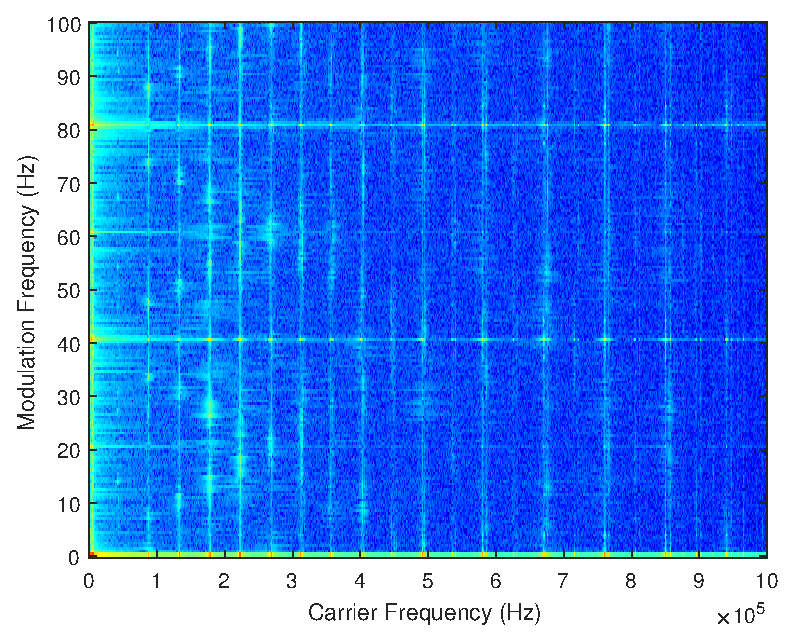
\includegraphics[width=\textwidth]{./dasp_algorithm_results/masp_low_filenum_9601.eps}
	\centering
	\caption{MASP output image derived from the time domain capture of the URE in Figure \ref{fig:hasp_fft_example}.  The vertical lines represent potential carriers across the entire capture spectrum and the horizontal lines represent amplitude modulations across the entire spectrum.  The intersection of these lines represents the location of a modulated carrier.  In addition to the strong frequency peaks identified in Figure \ref{fig:hasp_fft_example}, modulations frequencies can be found at $20$Hz and its respective harmonics.}
	\label{fig:masp_example}
\end{figure}

In addition to the modulations occurring at $20$Hz and its harmonics, several unrelated modulation and carrier frequency intersections were identified in Figure \ref{fig:masp_example}.  For instance, significant peaks were identified at the intersection of the fourth harmonic of the dominant carrier frequency, approximately $180$kHz, and modulations frequencies of $15$Hz and $25$Hz, indicating a strong amplitude modulation which was not identified during analysis of the HASP-F and HASP-D images.

\section[Spectral Correlation Aligned Projection (SCAP)]{Spectral Correlation Aligned Projection (SCAP)}
\label{Spectral Correlation Aligned Projection}

The SCAP algorithm provides a method for aligning frequency spacings between peaks in the frequency domain.  Fixed frequency spacings can result from frequency harmonics, frequency mixing, or frequency and amplitude modulations; and furthermore, can occur at multiple unrelated locations within the conducted URE spectrum. The SCAP algorithm provides two outputs, $\bf{S}_H$ and $\bf{S}_F$, where $\bf{S}_F$ is the autocovariance, $\bf{C}_{XX}$, of $\hat{r}$ and $\bf{S}_H$ results from the application of the HASP-D algorithm to $\bf{S}_F$, as described in Algorithm \ref{alg:scapalg}. 

\begin{algorithm}
	\caption{Spectral Correlation Aligned Projection Algorithm} \label{alg:scapalg}
	\scriptsize
	\begin{algorithmic}[1]
		\Require~~
		\Statex $\hat{r}$ - Input Power Spectrum
		\Ensure~~
		\Statex $\bf{S}_H$ - SCAP Output
		\Statex $\bf{S}_F$ - Spectral Autocovariance Vector 
		\Statex
		\State $\bf{S}_F \gets \bf{C}_{XX}(\hat{r})$
		\State $\bf{S}_H \gets $ HASP-D of $\bf{S}_F$ 
	\end{algorithmic}
\end{algorithm}

Figure \ref{fig:scap_xcov_example} shows the autocovariance of $\hat{r}$, $\bf{S}_F$, of the conducted URE spectrum illustrated in Figure \ref{fig:hasp_fft_example}, with $\bf{S}_H$ shown in Figure \ref{fig:scap_hasp_example} after application of the HASP-D algorithm.  The HASP-D algorithm was configured with $f_c = 1000$Hz and $B = 1900$Hz and a maximum harmonic of $K = 10$.  In addition, $\bf{S}_F$ was scaled such that the maximum peak value equals one and the frequency correlation axis was limited from $100$kHz to $70$Hz with a reverse semi-log scale.

\begin{figure}[tp]
	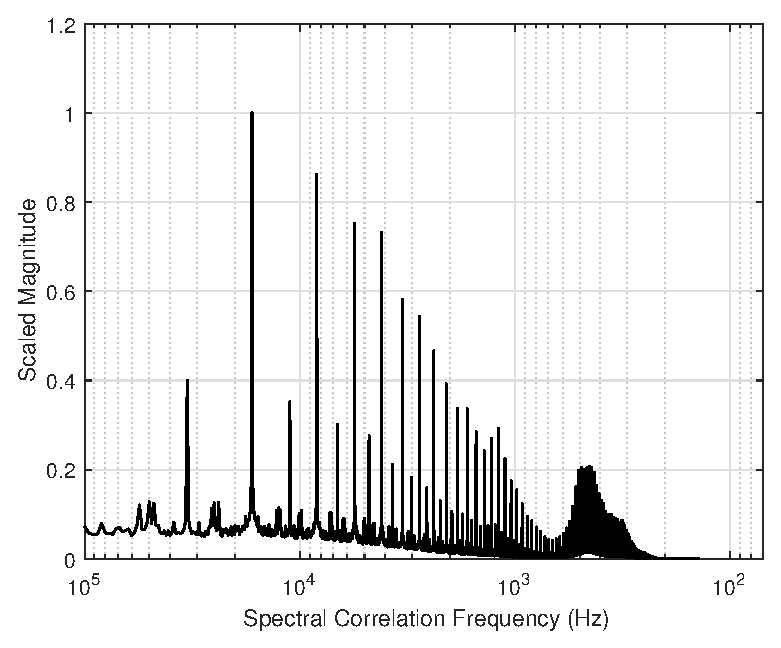
\includegraphics[width=\textwidth]{./dasp_algorithm_results/scap_filenum_12001.eps}
	\centering
	\caption{Plot of the autocovariance of the FFT shown in Figure \ref{fig:hasp_fft_example}.  The peaks within the plot represent the correlation of equally spaced frequency peaks within the FFT, with a dominant correlation at $16.67$kHz, which corresponds to roughly $120$ FFT bins.}
	\label{fig:scap_xcov_example}
\end{figure}

\begin{figure}[tp]
	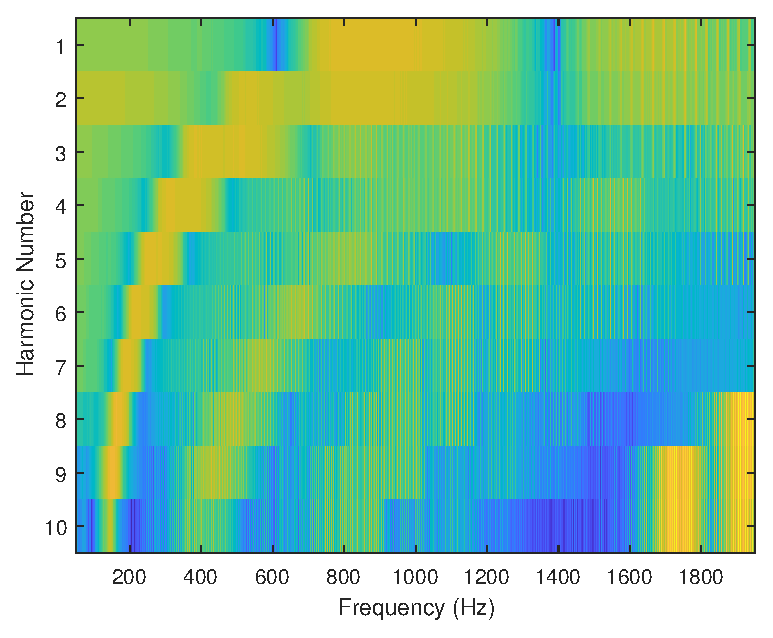
\includegraphics[width=\textwidth]{./dasp_algorithm_results/scap_hasp_filenum_12001.eps}
	\centering
	\caption{SCAP image, $\bf{S}_H$, generated by applying the HASP-D algorithm to the autocovariance vector, $\bf{S}_F$, shown in Figure \ref{fig:scap_xcov_example}.}
	\label{fig:scap_hasp_example}
\end{figure}

Figure \ref{fig:scap_xcov_example} shows a significant number of correlation peaks resulting from the equal spacing of peaks within the frequency spectrum of $\hat{r}$.  The dominant peak occurs at $16$kHz along with corresponding sub-correlations at integer divisions of $16$kHz.  An additional unrelated correlation ``hump'' occurs between $200$Hz and $400$Hz.  Although the previously identified oscillator frequencies from Figure \ref{fig:hasp_fft_example} resulted in significant peaks in the FFT spectrum, the correlation spectrum did not return a strong response, although still identifiable at a much lower level.   This was likely due to the low frequency instability in the signals, identified in Figure \ref{fig:haspd_example_zoom}, as well as the close proximity of the two oscillators resulting in a diminished correlation value.

\section[Cross-Modulation Aligned Signal Projection (CMASP)]{Cross-Modulation Aligned Signal Projection (CMASP)}
\label{Cross-Modulation Aligned Signal Projection}

In addition to carrier frequencies having significant harmonic content, modulation sidebands around a given carrier frequency and its respective harmonics can also have significant harmonic content.  The CMASP algorithm was developed to find the intersection of carrier and modulation frequencies, much like the MASP algorithm, but also provide a mechanism for highlighting the harmonic content of the modulation sidebands, such as the harmonics of $20$Hz previously noted in Figure \ref{fig:masp_example}.  Figure \ref{fig:cmasp_diagram} provides a graphical depiction of the CMASP process as applied to a nominal FFT spectrum.   The CMASP process sweeps across all potential carrier frequencies within a band of interest and provides a sum of the power spectrum of a given carrier frequency and its harmonics, much like the HASP process, but also includes a summation of modulation frequency sidebands and related harmonics.  The CMASP process results in a modulation frequency by carrier frequency image with an ``X'' and associated peaks corresponding to the intersection of a carrier and modulation frequency and their respective harmonics.

\begin{figure}[tp]
	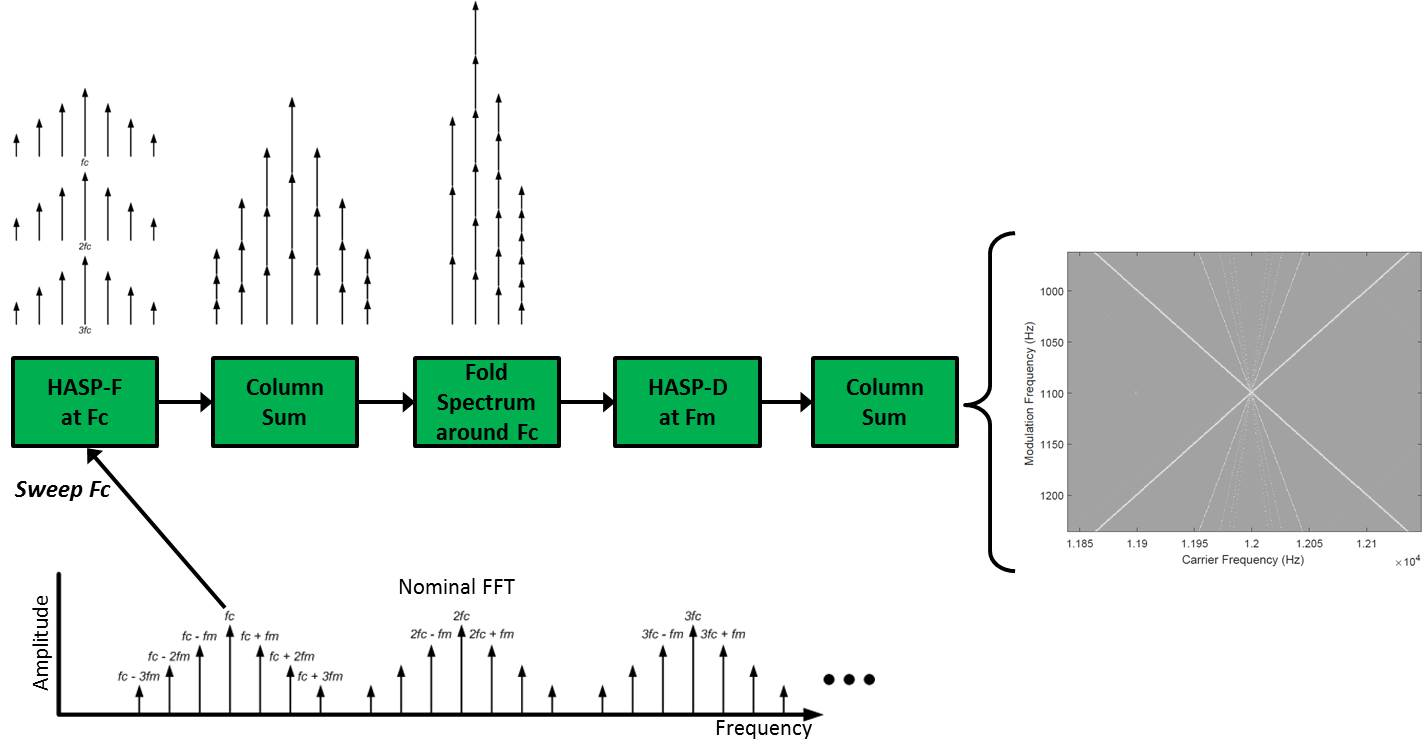
\includegraphics[width=\textwidth]{./misc_graphics/cmasp_diagram.jpg}
	\centering
	\caption{Diagram of the CMASP process as applied to a signal with a carrier frequency ($f_c$) and modulation frequency sidebands ($f_m$), where $f_c$ and $f_m$ both have harmonic content.  The CMASP process sweeps across $f_c$ and aligns the harmonics of the modulation frequency to highlight the intersection of carrier and modulation frequencies.}
	\label{fig:cmasp_diagram}
\end{figure}

The CMASP process is described further in Algorithm \ref{alg:cmaspalg}.  The CMASP process operates on an input signal's power spectral density, $\hat{r}$, and requires carrier center frequency ($f_c$), carrier frequency bandwidth ($B_c$), modulation center frequency ($f_m$), and modulation frequency bandwidth ($B_m$) inputs.  The algorithm initially performs the HASP-F algorithm on $\hat{r}$ and sums all columns in to a 1-D vector.  The 1-D vector is then folded around the center frequency bin and summed to add the lower and upper sideband components.  The HASP-D algorithm is applied to the folded and summed vector to align the harmonics of the modulation frequency.  Finally, the HASP-D output is summed along all columns with the resulting vector forming a single column in the CMASP image.  The process is repeated for all frequency bins within the carrier frequency bandwidth to form a modulation frequency by carrier frequency matrix, with dimensions of $f_m \pm B_m$ by $f_c \pm B_c$, respectively. 

\begin{algorithm}
	\caption{Cross-Modulation Aligned Projection Algorithm} \label{alg:cmaspalg}
	\scriptsize
	\centering
	\begin{algorithmic}[1]
		\Require~~
		\Statex $\hat{r}$ - Input Power Spectrum
		\Statex $f_c$ - Carrier Center Frequency 
		\Statex $f_m$ - Modulation Center Frequency 
		\Statex $B_c$ - Carrier Frequency Bandwidth
		\Statex $B_m$ - Modulation Frequency Bandwidth
		\Ensure~~
		\Statex $\bf{C}$ - CMASP Output Array
		\Statex
		\ForAll  {$i$, where $(k \times f_c) - B/2 \leq f_i \leq (k \times f_c) + B/2$} 
		\State    $\bf{C_m} \gets $ HASP-F($\hat{r}$, $f_i$, $B_c$)
		\State 		$\bf{C_m} \gets $ COLUMN SUM of $\bf{C_m}$
		\State 		$\bf{C_m} \gets \bf{C_m}$(END$/2$ to $1$) + $\bf{C_m}$(END$/2$ to END)
		\State		$\bf{C_m} \gets $ COLUMN SUM of HASP-D($\bf{C_m}$, $f_m$, $B_m$)
		\State		$i$-th column of $\bf{C} \gets \bf{C_m}$
		\EndFor
	\end{algorithmic}
\end{algorithm}

To illustrate the CMASP output, a synthetic signal was generated by amplitude modulating a square wave at a frequency of $12$kHz with a square wave at $1100$Hz.  The resulting power spectral density of the synthetic signal consisted of multiple harmonics of the $12$kHz carrier signal along with multiple upper and lower sidebands comprised of the $1100$Hz modulating frequency and its corresponding harmonics.   Figure \ref{fig:cmasp_synth_example} shows the output of the CMASP process as applied to the synthetic test signal.   The large ``X'' within the image is the result of the intersection of the carrier frequency and the fundamental modulation frequency.  The additional radials at progressively smaller angles are the result of sidebands from the modulation frequency harmonics.  Furthermore, the left-right mirrored radials are due to the presence of both upper and lower modulation sidebands.  Analysis of Figure \ref{fig:cmasp_synth_example} therefore shows a $12$kHz carrier signal being modulated by a $1100$Hz signal with both upper and lower sidebands and multiple harmonics.

\begin{figure}[tp]
	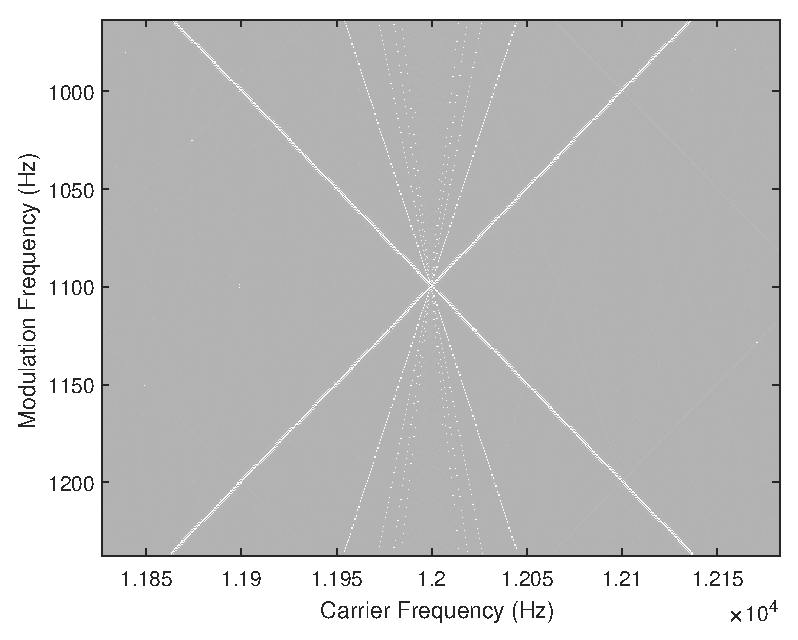
\includegraphics[width=\textwidth]{./dasp_algorithm_results/cmasp_synth.eps}
	\centering
	\caption{CMASP output image resulting from application of the CMASP algorithm to synthetic data.  The synthetic data was generated by multiplying a $1100$Hz square wave with a $12$kHz square wave carrier frequency.  The ``X'' represents the intersection of a modulation frequency at $1100$Hz and its harmonics with a carrier frequency at $12$kHz.}
	\label{fig:cmasp_synth_example}
\end{figure}

Figure \ref{fig:cmasp_example} shows the CMASP algorithm applied to the conducted URE signal from the fluorescent lights as shown in Figure \ref{fig:hasp_fft_example}.  Several radials and intersections are identifiable, with the most prominent occurring at $120$Hz and its respective harmonics.  Single lines appearing with no obvious intersection with a mirrored radial are likely due to unmodulated frequency peaks within the spectrum.
 
\begin{figure}[tp]
	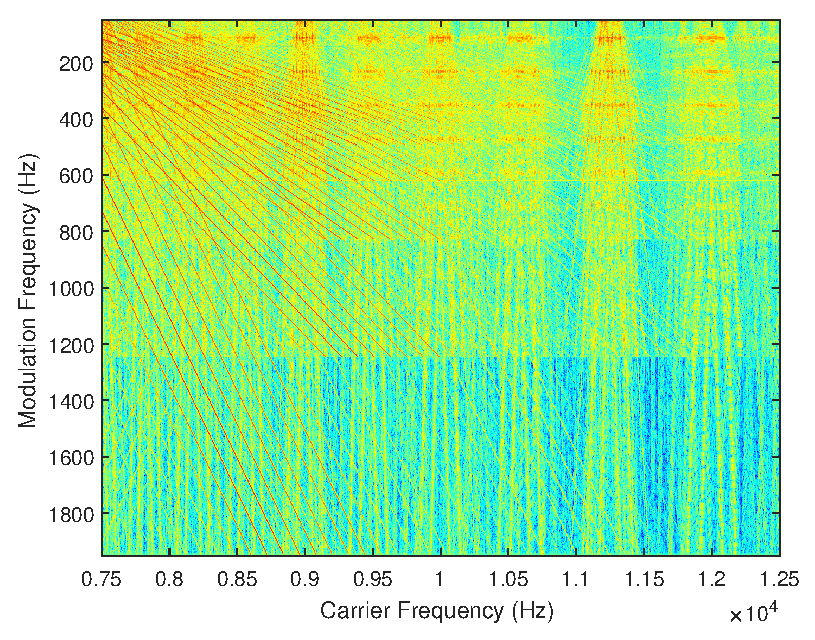
\includegraphics[width=\textwidth]{./dasp_algorithm_results/cmasp_filenum_9601.eps}
	\centering
	\caption{CMASP output image resulting from the fluorescent light conducted URE spectrum shown in Figure \ref{fig:hasp_fft_example}.}
	\label{fig:cmasp_example}
\end{figure}

\section[Frequency Aligned Signal Projection (FASP)]{Frequency Aligned Signal Projection (FASP)}
\label{Frequency Aligned Signal Projection}

The FASP algorithm performs FFTs on short time segments of a time domain signal and aligns the frequency bins of each processed time slice, as detailed in Algorithm \ref{alg:faspalg}.  The FASP algorithm operates on a time domain input signal, $r$, and only requires the number of times slices, $N$, as an input parameter.  Given a fixed length capture, with capture time, $T_c$, and sample rate, $F_s$, the FASP algorithm returns a time by frequency image with dimensions of $\frac{T_c}{N}$ seconds by $\frac{F_s}{2}$Hz.

\begin{algorithm}
	\caption{Frequency Aligned Signal Projection Algorithm} \label{alg:faspalg}
	\scriptsize
	\begin{algorithmic}[1]
		\Require~~
		\Statex $r$ - Input Time Domain Signal
		\Statex $N$ - Number of Time Slices of a Fixed Length Capture File
		\Ensure~~
		\Statex $\mathbf{F}$ - FASP Output Array
		\Statex
		\For  {$n = 1, 2, \ldots N$} 
		\State Row $n$ of $\mathbf{F} \gets $ FFT of $r(x_i)$ where, $(n - 1)T_c/N < x_i < nT_c/N$
		\EndFor
		\State $\mathbf{F} \gets \left|\bf{F}\right|$
	\end{algorithmic}
\end{algorithm}

Figure \ref{fig:fasp_example} shows the FASP algorithm applied to same time domain URE capture represented in Figure \ref{fig:hasp_fft_example}.  As previously noted, the separation of the two fluorescent light $45$kHz oscillator harmonics can be seen at the higher frequencies.   Although not as clear, a slight ``wobble'' on the fundamental frequency and its harmonics can be seen over time resulting from the low frequency modulations identified in Figure \ref{fig:haspd_example_zoom} and Figure \ref{fig:masp_example}.  Given a capture time of one second and a sample rate of $2$MS/s, each row represents a $0.2$ms time slice with the frequency axis spanning $0$ to $1$MHz.
 
\begin{figure}[tp]
	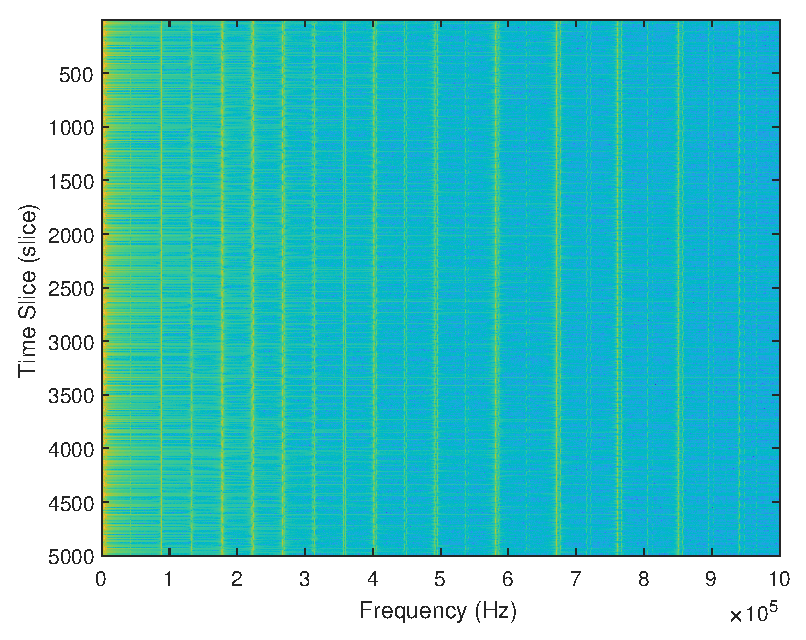
\includegraphics[width=\textwidth]{./dasp_algorithm_results/fasp_filenum_9601.eps}
	\centering
	\caption{FASP algorithm applied to the conducted URE signal illustrated in Figure \ref{fig:hasp_fft_example}.  The $45$kHz carriers and respective harmonics are clearly seen throughout the spectrum on all time slices, with the spacing between their harmonics progressively increasing.}
	\label{fig:fasp_example}
\end{figure}
    
% To compile single chapters put a % symbol in front of "\comment" and "}%end of comment" below 
%    and take off the % symbol from "\end{document" at the bottom line. Undo before compiling
%    the complete thesis
%%Note: You can only use \section command, you are not allowed, per TTU Graduate School, use
%%\subsection command for ghigher level subheadings. At most level 2 subheadings are allowed.

\chapter{DASP Image Processing and Feature Extraction}
\label{DASP Feature Extraction Chapter}

\section[DASP Image Pre-Processing]{DASP Image Pre-Processing}
\label{DASP Image Pre-Processing Section}

The suite of DASP algorithms presented in Chapter \ref{DASP Algorithm Development Chapter} provide methods for aligning and highlighting signal dimensions, such as modulations and harmonics, that are inherent to URE conducted from electronic equipment.  The resulting alignments can take a variety of shapes within the DASP images, from straight lines to curved lines to crossing radials to signal peaks; however, direct feature extraction from the raw DASP images can be problematic because of scaling, dynamic range, and confounding signal structures.

Multiple image processing and feature extraction techniques were utilized to prepare the DASP images for machine learning analysis.  Two machine learning techniques were explored, a feature vector based approach and an image classification learning method, with both requiring different DASP image pre-processing methods.  Both learning methods required the DASP images to be scaled to limit dynamic range and remove the background noise, as outlined in Section \ref{Image Scaling}.  To further highlight features of interest, such as lines and peaks, the raw DASP images were also processed with thresholding, edge, and line detection algorithms, as described in Sections \ref{Threshold Processing} and \ref{Edge and Line Detection}.  The image classification technique operated directly on the scaled and processed images with no further feature extraction required, whereas the DASP images were further processed through an image segmentation, matrix summing, and statistical measurement process to form feature vectors for the feature vector machine learning algorithms, as outlined in Sections \ref{Image Segmentation} and \ref{Statistical Feature Extraction}.

\subsection[Image Scaling]{Image Scaling}
\label{Image Scaling}

DASP images can suffer from dynamic range issues resulting from the large differences ($10$s of dB) in measured URE signal levels from a single device or across multiple devices, which can further be exacerbated by the bit growth associated with the continual multiplication and summing steps that comprise the DASP processes.  In addition, different parts of a given URE spectrum can vary widely because of broadband noise or narrowband frequency peaks unrelated to the device under test.  To normalize and scale DASP images before further image processing or feature extraction the image scaling algorithm described in Algorithm \ref{alg:imscalealg} was initially applied to all DASP generated images. 

\begin{algorithm}
	\caption{Image Scaling Algorithm} \label{alg:imscalealg}
	\scriptsize
	\begin{algorithmic}[1]
		\Require~~
		\Statex $\mathbf{I}$ - Input Image
		\Statex $\mathbf{I_b}$ - Background Image
		\Ensure~~
		\Statex $\mathbf{I_s}$ - Scaled Image Output
		\Statex
		\State $\mathbf{I_s} \gets \mathbf{I} - \mathbf{I_b}$ 
		\State $\mathbf{I_s} \leq 0 \gets 0$
		\State $\mathbf{I_s}  \gets $ STANDARD DEVIATION FILTER of $\mathbf{I_s}$
		\State $\mathbf{I_s} = \log{\mathbf{I_s}}$
	\end{algorithmic}
\end{algorithm}

The URE collection process outlined in Chapter \ref{URE Data Collection Chapter} recorded $24000$ \textit{off} state captures of which $22800$ were randomly selected and removed from the test and training data set to generate a representative background for DASP device image normalization.  The removal of the extra \textit{None} state captures also balanced the number of samples per class and eliminated any concerns regarding class skew in the learning process.  The $22800$ \textit{off} state DASP images were averaged together to form a background image, $\bf{I_b}$, which was subtracted from the raw DASP images, $\bf{I}$, to generate a scaled image, $\bf{I_s}$.   A rectifying linear transformation was then applied to $\bf{I_s}$ followed by a standard deviation image filter resulting in a localized z-score across the entire image.  Finally, a logarithm was applied to each pixel of entire image to further reduce the dynamic range of the scaled image.  

\subsection[Threshold Processing]{Threshold Processing}
\label{Threshold Processing}

The MASP algorithm was specifically developed to generate a peak at the intersection of a modulation frequency and carrier frequency.  These peaks are often obscured within the MASP image because of a large dynamic range or by being masked by unmodulated portions of a carrier frequency, as can be seen in Figure \ref{fig:masp_example}.  To highlight peaks within a MASP image a threshold processing algorithm was developed to generate a scatter plot with each scatter point representing a detected peak in the original image.  The algorithm is described in Algorithm \ref{alg:scatteralg} and operates on an input MASP image, $\mathbf{I}$, with the fill ratio, $p$, input parameter which determines the total number of scatter points to generate in the final scatter plot.   

\begin{algorithm}
	\caption{Scatter Plot Peak Detection Algorithm} \label{alg:scatteralg}
	\scriptsize
	\begin{algorithmic}[1]
		\Require~~
		\Statex $\mathbf{I}$ - Input Image
		\Statex $p$ - Fill Ratio
		\Ensure~~
		\Statex $\mathbf{S}$ - Detected Scatter Points
		\Statex
		\Statex Initialize THRESHOLD 
		\While {$1.1p < $ fill $ < 0.9p$}
			\State $\bf{I_t} \gets $ ZSCORE for each row of $\bf{I}$
			\State $\bf{I_t} \gets 0$ for all $\bf{I_t} \le$ THRESHOLD
			\State $\bf{I_t} \gets $ ZSCORE for each column of $\bf{I_t}$ for all $\bf{I_t} \ne 0$
			\State INITIALIZE $\bf{S} = 0$
			\For {elements of $\bf{I_t} \geq $ THRESHOLD}
				\State $\mathbf{S} \gets 1$
			\EndFor
			\State fill $ \gets \sum{\bf{S}}$
			\State UPDATE THRESHOLD
		\EndWhile
	\end{algorithmic}
\end{algorithm}

The scatter plot algorithm initializes a threshold which is iterated on until the number of scatter points is within $10\%$ of the fill ratio.  The algorithm separately scales and thresholds the rows and columns of an image to only generate scatter points that exceed a given threshold in both directions.  After thresholding, the total number of scatter points is calculated and the threshold value is updated to either increase or decrease the number of scatter points based upon the difference between the fill ratio and the total number of scatter points in the current iteration.

To illustrate the scatter point threshold algorithm and image output, the scatter plot peak detection algorithm was applied to the MASP image in Figure \ref{fig:masp_example} and is shown in Figure \ref{fig:maspl_scatter}.  The scatter plot shows groupings, rows, and columns of scatter points that identify modulation peaks that were not easily identifiable in the original MASP image.  For instance, the row of points at $f_m = 26$Hz indicate a significant number of higher frequency carriers being modulated by $26$Hz, which is not obvious in the original MASP image in Figure \ref{fig:masp_example}.

\begin{figure}[tb]
	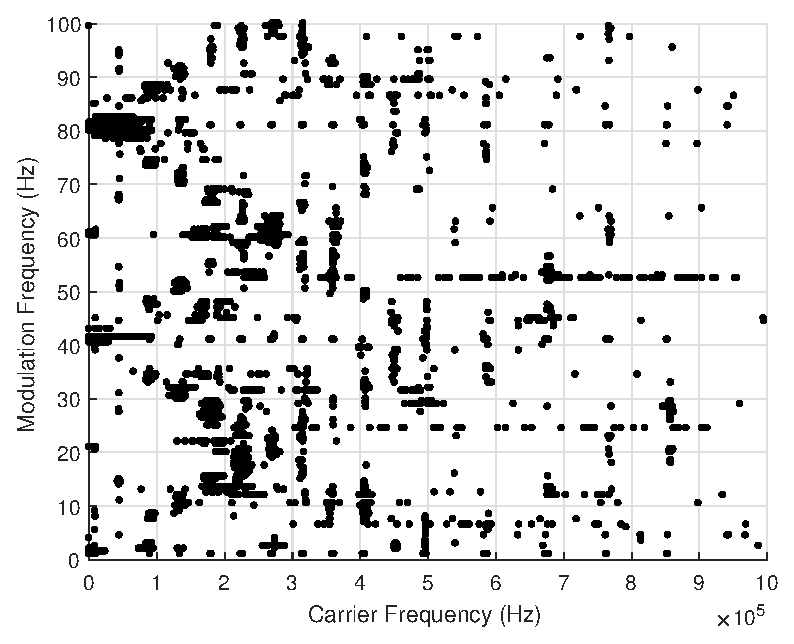
\includegraphics[width=\textwidth]{./dasp_algorithm_results/masp_low_scatter_filenum_12001.eps}
	\centering
	\caption{Scatter plot resulting from the peak thresholding of the MASP image in Figure \ref{fig:masp_example}.  The scatter plot highlights peaks in the MASP image that would otherwise not be visible due to dynamic range of the image, such as the row of points located at the $26$Hz modulation frequency.  It should also be noted that the horizontal lines at $20$Hz and $60$Hz in Figure \ref{fig:masp_example} are no longer visible because their magnitudes did not exceed the threshold in both the vertical and horizontal dimensions.}
	\label{fig:maspl_scatter}
\end{figure}

In addition to the row of modulations at $26$Hz, its second harmonic at $52$Hz also showed a similar broadband modulation pattern.  Several modulation structures became evident upon further examination, such as the large clustering of modulations at the intersection of $80$Hz with low frequency carriers and the large number of clusters between the $100$kHz and $200$kHz carrier frequencies.  By performing the scatter point thresholding against the rows and columns of the MASP image, the resulting scatter plot can highlight modulation structures that are not evident in the raw images.   

\subsection[Edge and Line Detection]{Edge and Line Detection}
\label{Edge and Line Detection}

Several of the DASP algorithms result in images that contain dimensional alignments that generate straight and curved lines, such as with HASP and CMASP, and much like the scatter plot peak detection algorithm for the MASP images, tailored transforms were required to highlight and exploit these features.  To highlight lines and edges within a DASP image a Laplacian of Gaussian (LoG) edge detector \cite{Marr1980} was applied to the DASP images using the MATLAB\textsuperscript \textregistered ~ \textit{edge} function\footnote{https://www.mathworks.com/help/images/ref/edge.html, June $26$, $2017$}.  Figure \ref{fig:cmasp_edge} shows the resulting image after application of the LoG edge detector to the image in Figure \ref{fig:cmasp_example} while using a LoG filter standard deviation value of $2$ and a filter size of $13 \times 13$.  

\begin{figure}[tb]
	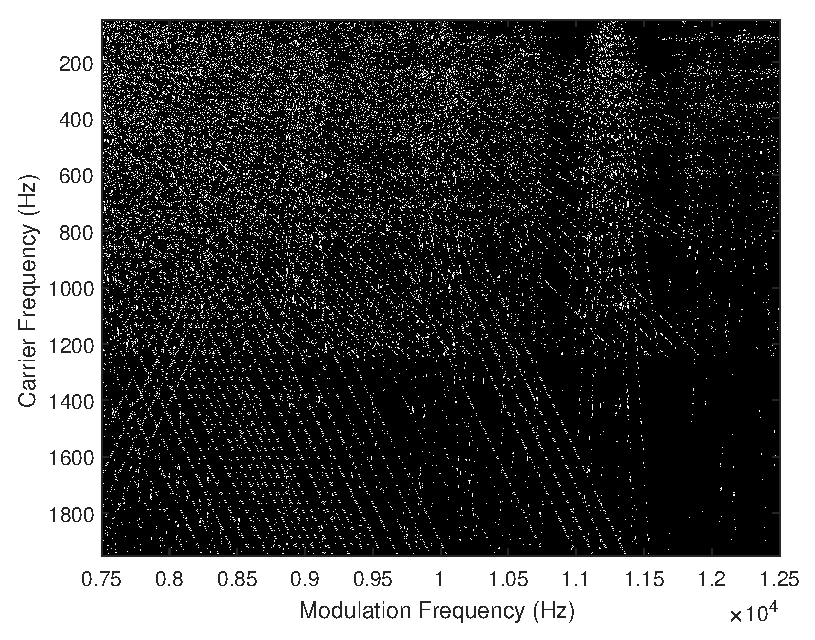
\includegraphics[width=\textwidth]{./dasp_algorithm_results/cmasp_edge_filenum_9601.eps}
	\centering
	\caption{CMASP image resulting from the application of a LoG edge detector to the image in Figure \ref{fig:cmasp_example}.  The edge detection algorithm removes variations in the background and highlights edges and lines for subsequent feature extraction or line detection processing.}
	\label{fig:cmasp_edge}
\end{figure}

Application of the LoG edge detector highlighted discontinuities in the processed image, resulting in an image with detection points forming lines and other shapes outlining the structures within the original image.  A radon transform \cite{Deans1981} was then applied to the CMASP edge detection image, Figure \ref{fig:cmasp_edge}, to detect radial lines traversing the image, as shown in Figure \ref{fig:cmasp_radon}.  The MATLAB\textsuperscript \textregistered ~ \textit{radon} function \footnote{https://www.mathworks.com/help/images/ref/radon.html, June $26$, $2017$} was utilized with projection angles between $0^{\circ}$ and $180^{\circ}$.  Figure \ref{fig:cmasp_radon} shows the radon output image along with detected peaks highlighted with circles, while Figure \ref{fig:cmasp_peak} provides a mesh plot of the same image to better illustrate image peaks.  Each peak in the radon image corresponds to a detected line at a given location ($x'$) and angle.
  
\begin{figure}[tb]
	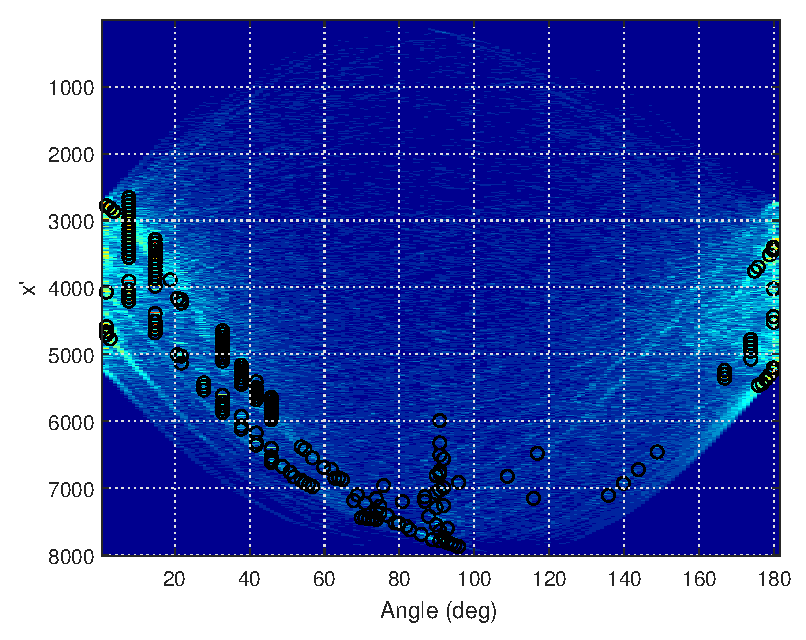
\includegraphics[width=\textwidth]{./dasp_algorithm_results/cmasp_radon_filenum_9601.eps}
	\centering
	\caption{Radon transform of the CMASP image in Figure \ref{fig:cmasp_edge} with detected peaks highlighted with circles.  Each detected peak corresponds to a line in the original image.  The vertically aligned circles in the center of the image correspond to vertical lines in the original image and the circles in the left and right quadrants correspond to angled lines in the original image with the x-axis providing the angle and the y-axis the location.}
	\label{fig:cmasp_radon}
\end{figure}

\begin{figure}[tb]
	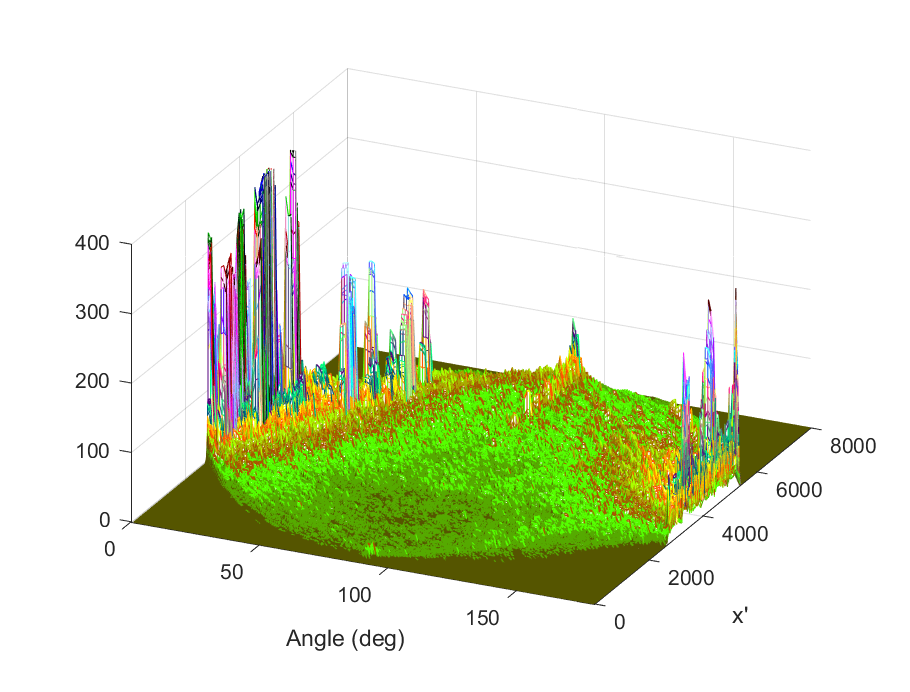
\includegraphics[width=\textwidth]{./dasp_algorithm_results/cmasp_radon_mesh_filenum_9601.eps}
	\centering
	\caption{Mesh plot of the radon transformed CMASP image in Figure \ref{fig:cmasp_edge} illustrating the detected peaks.}
	\label{fig:cmasp_peak}
\end{figure}

The LoG and radon functions provide a suite of tools for highlighting lines and edges within a DASP image.  As can be seen in Figure \ref{fig:cmasp_example}, the CMASP transform can generate many lines with no clear structure which could potentially confound and mask underlying discriminative features.  The application of the LoG edge detector can eliminate much of the underlying noise and highlight lines and edges of interest, while the subsequent application of the radon transform can detect highlighted lines and potentially provide a more compact representation of the CMASP image structure.  For instance, the large number of detected peaks in Figure \ref{fig:cmasp_radon} provided indications of a large number of distinct and left-to-right downward sloping lines, as evident in Figure \ref{fig:cmasp_edge}.

\subsection[Images Segmentation]{Image Segmentation}
\label{Image Segmentation}

Dimensional alignments or other features of interest relevant for the classification of URE generators occur within different regions of the DASP images.  To aid in feature extraction and to isolate features of interest, an image segmentation process was developed to generate sub-segments of an input DASP image.  The image segments are illustrated in Figure \ref{fig:haspd_segment}.  The segmentation of Figure \ref{fig:haspd_example} shows the isolation of aligned harmonics in segments $8$, $5$, and $2$.  In addition, the process also generated segments which did not contain features of interest for this particular device; however, other devices may generate features that do occur in these segments and therefore provide better discrimination for the purposes of classification. 

\begin{figure}[tb]
	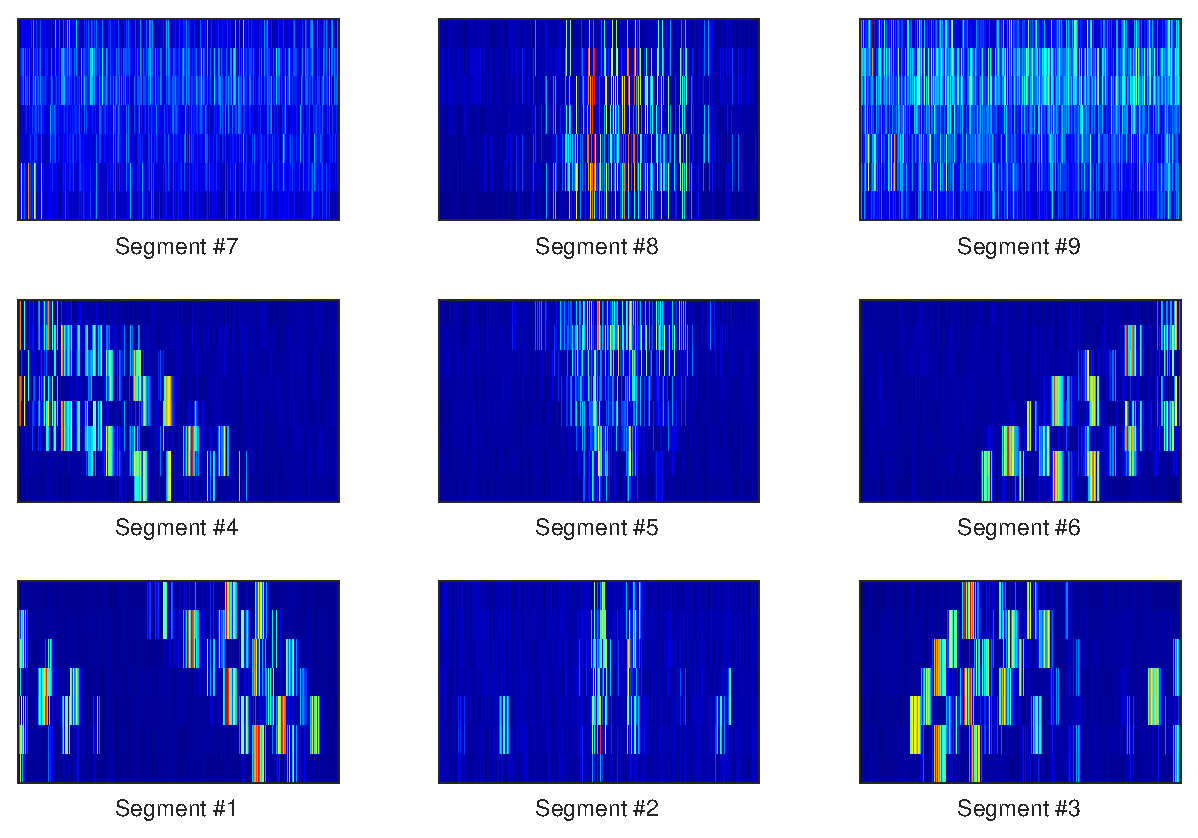
\includegraphics[width=\textwidth]{./dasp_algorithm_results/hasp_segment_filenum_12001.eps}
	\centering
	\caption{$3 \times 3$ image segmentation of the image in Figure \ref{fig:haspd_example} demonstrating the isolation of specific regions of interest.  By segmenting the image, features of interest can further be highlighted without confounders, such as in the center-bottom tile, segment $\#2$.}
	\label{fig:haspd_segment}
\end{figure}

\section[Statistical Feature Extraction]{Statistical Feature Extraction}
\label{Statistical Feature Extraction}

Extraction of features from the DASP images can be tailored to a specific device or class given \emph{a priori} knowledge of the URE characteristics, such as specific frequency peaks or modulation frequencies.  Given no prior knowledge of a device's URE characteristics and the low noise collection environment, no tailored feature extractors were utilized in the feature generation process.  Two machine learning classification techniques are explored in Chapter \ref{DASP Device Classification Chapter}. The first machine learning approach was based upon 1-D statistical feature vectors extracted from DASP images, while the second machine learning technique used was the CNN deep learning approach applied directly to the DASP images.   

General statistical features based on variance ($\sigma^2$), skewness ($\gamma$), and kurtosis ($\kappa$), as defined by Equations \ref{eq:sigmaeq}, \ref{eq:gammaeq}, and \ref{eq:kappaeq}, respectively, were extracted from the DASP images to form a 1-D feature vector for machine learning, as also demonstrated by \cite{Zhenfei2009}, \cite{Klein2009}, \cite{Lukacs2016}, and \cite{Cobb2010}.  Samples over which to compute the statistics were taken from the summed rows and columns of each image, or image segment, as illustrated in Figure \ref{fig:haspd_summation}.  For whole image feature extraction, all of the pixels of the image were concatenated into a single vector and used as samples for statistical feature generation.  

\begin{equation}
	\sigma^{2}_{\bf{x}} = \textbf{E}[(\textbf{x} - \mu)^2]
	\label{eq:sigmaeq}
\end{equation}

\begin{equation}
	\gamma_{\bf{x}} = \textbf{E}\left[\left(\frac{\textbf{x} - \mu}{\sigma}\right)^3\right]
	\label{eq:gammaeq}
\end{equation}

\begin{equation}
	\kappa_{\bf{x}} = \frac{\textbf{E}[(\textbf{x} - \mu)^4]}{(\textbf{E}[(\textbf{x} - \mu)^2])^2}
	\label{eq:kappaeq}
\end{equation}

where $\bf{x}$ are the samples taken from the summed rows, summed columns, and concatenated pixel vector of the DASP arrays shown in Figure \ref{fig:haspd_summation}.

\begin{figure}[ht]
	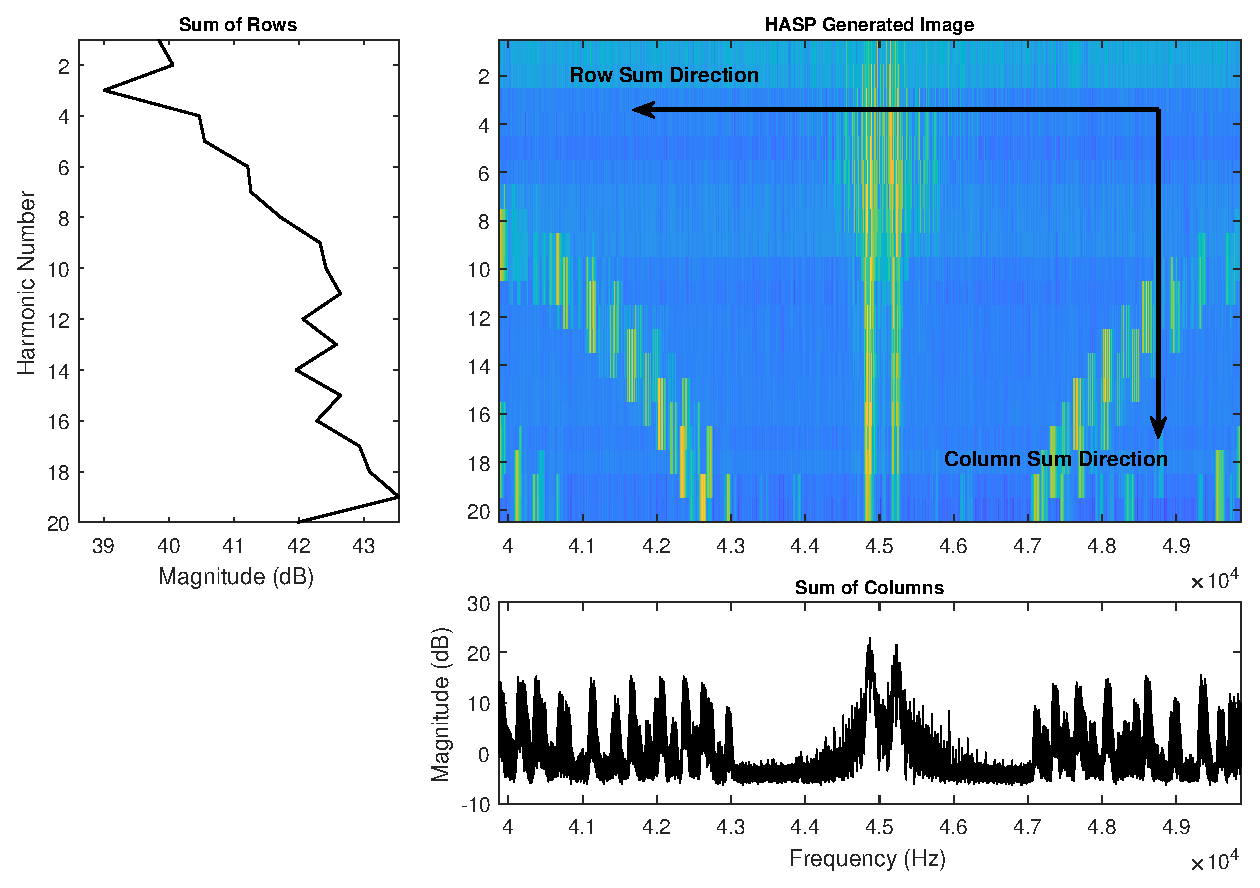
\includegraphics[width=\textwidth]{./dasp_algorithm_results/hasp_d_summing_filenum_9601.eps}
	\centering
	\caption{Column and row summing as applied to the HASP-D image shown in Figure \ref{fig:haspd_example}.  By aligning the independent carriers and their respective harmonics in the HASP-D image, the column summing provides a method for adding the ``coherent'' energy associated with the independent carriers, providing a significant response in the resulting summed vector.}
	\label{fig:haspd_summation}
\end{figure}

As illustrated in Figure \ref{fig:haspd_summation}, the HASP-D algorithm aligns harmonically related frequencies into a single column within the HASP-D image and the column summing allows all of the related harmonics to be added coherently into a single vector as demonstrated in the sum of columns plot.   Although not as pronounced in Figure \ref{fig:haspd_summation}, the row summing can provide insights into the harmonic structure of the underlying signal.  For instance, the summed row vector shows an alternating harmonic intensity structure between the $11$th and $17$th harmonics.

%\section[Image Structural Similarity]{Image Structural Similarity}
%
%\blindtext[1]
%
%\begin{equation}
	%SSIM(x,y) = \left[i(x,y)\right]^{\alpha}\left[c(x,y)\right]^{\beta}\left[S(x,y)\right]^{\gamma} 
	%\label{eq:ssimeq}
%\end{equation}
%
%where
%
%\begin{equation}
	%i(x,y) = \left[i(x,y)\right]^{\alpha}\left[c(x,y)\right]^{\beta}\left[s(x,y)\right]^{\gamma} 
	%\label{eq:ssimieq}
%\end{equation}
%
%\begin{equation}
	%c(x,y) = \frac{2\mu_{x}\mu_{y} + C_{1}}{\sigma^{2}_{x} +\sigma^{2}_{y} + C_{2}}
	%\label{eq:ssimceq}
%\end{equation}
%
%\begin{equation}
	%s(x,y) = \left[i(x,y)\right]^{\alpha}\left[c(x,y)\right]^{\beta}\left[S(x,y)\right]^{\gamma} 
	%\label{eq:ssimseq}
%\end{equation}
%
%\begin{figure}[ht]
	%\includegraphics[width=\textwidth]{./dasp_algorithm_results/masp_refimage_ssim_device_6.eps}
	%\centering
	%\caption{Reference MASP image generated by averaging $20$ MASP images derived from URE collected from fluorescent lights and subtracting the background (i.e. the ``None'' state).}
	%\label{fig:masp_ref_image}
%\end{figure}
%
%\begin{figure}[ht]
	%\includegraphics[width=\textwidth]{./dasp_algorithm_results/masp_image_ssim_refcmp_device_6.eps}
	%\centering
	%\caption{Plot of structural similarity index values between MASP reference image of device $6$ and a random sampling of MASP images from all $20$ devices.  The peak at $6$ shows the highest similarity to device $6$, which confirms the applicability of comparing DASP images through SSIM values.}
	%\label{fig:masp_ssim_dev}
%\end{figure}
%
%\begin{figure}[ht]
	%\includegraphics[width=\textwidth]{./dasp_algorithm_results/masp_image_ssim_multrefcmp_device_6.eps}
	%\centering
	%\caption{Image of SSIM values using a comparison of the MASP reference image for device $6$ to captures with all combinations of two devices present.  The peaks at the rows and columns at $6$ show that even with confounders the SSIM still shows a peak when device $6$ is present and further shows that the SSIM to all other combinations of devices is low.}
	%\label{fig:masp_ssim_multi}
%\end{figure}



%\begin{figure}[ht]
	%\includegraphics[width=\textwidth]{./dasp_algorithm_results/masp_summing_filenum_9601.eps}
	%\centering
	%\caption{Column and row summing as applied to the MASP image shown in \ref{fig:masp_example}.  The row summing highlights the relative strengths and location of the modulating frequencies.}
	%\label{fig:masp_summation}
%\end{figure}

%\subsubsection[Clustering Analysis]{Cluster Analysis}
%
%\blindtext[1]
%
%\begin{figure}[ht]
	%\includegraphics[width=\textwidth]{./dasp_algorithm_results/masp_dbscan_noise_filenum_12001.eps}
	%\centering
	%\caption{MASP Scatter DBSCAN with Noise}
	%\label{fig:maspdbscannoise}
%\end{figure}
%
%\begin{figure}[ht]
	%\includegraphics[width=\textwidth]{./dasp_algorithm_results/masp_dbscan_nonoise_filenum_12001.eps}
	%\centering
	%\caption{MASP Scatter DBSCAN without Noise}
	%\label{fig:maspdbscanwithoutnoise}
%\end{figure}
%
%\begin{figure}[ht]
	%\includegraphics[width=\textwidth]{./dasp_algorithm_results/masp_blob_area_filenum_12001.eps}
	%\centering
	%\caption{MASP Blob analysis with detected corners}
	%\label{fig:maspblob}
%\end{figure}
%
%\begin{figure}[ht]
	%\includegraphics[width=\textwidth]{./dasp_algorithm_results/hasp_dbscan_nonoise_filenum_12001.eps}
	%\centering
	%\caption{HASP Scatter DBSCAN without Noise}
	%\label{fig:haspdbscanwithoutnoise}
%\end{figure}
%
%\begin{figure}[ht]
	%\includegraphics[width=\textwidth]{./dasp_algorithm_results/hasp_blob_area_filenum_12001.eps}
	%\centering
	%\caption{HASP Blob analysis with detected corners}
	%\label{fig:haspblob}
%\end{figure}
%\subsection[Histogram Based Features]{Histogram Based Features}
%
%\begin{figure}[ht]
	%\includegraphics[width=\textwidth]{./dasp_algorithm_results/masp_hist_filenum_12001.eps}
	%\centering
	%\caption{MASP Aligned Histogram}
	%\label{fig:masphist}
%\end{figure}
%
%\begin{figure}[ht]
	%\includegraphics[width=\textwidth]{./dasp_algorithm_results/masp_segment_filenum_12001.eps}
	%\centering
	%\caption{$3 \times 3$ image segmentation of the \ref{fig:masp_summation} image isolating specific regions of interest.  Tiling of the MASP image highlights specific locations of peaks associated with the intersection of carrier and modulation frequencies, such as illustrated in the top two rows of tiles.} 
	%\label{fig:masp_segment}
%\end{figure}


   
% To compile single chapters put a % symbol in front of "\comment" and "}%end of comment" below 
%    and take off the % symbol from "\end{document" at the bottom line. Undo before compiling
%    the complete thesis
%%Note: You can only use \section command, you are not allowed, per TTU Graduate School, use
%%\subsection command for ghigher level subheadings. At most level 2 subheadings are allowed.

\chapter{Test and Evaluation Configuration}
\label{Simulation and Testing Configuration}

\section[Simulation Overview]{Testing Overview}

Two machine learning approaches are utilized in Chapter \ref{DASP Device Classification Chapter} to determine the performance and applicability of DASP originated features for URE characterization and classification.  A feature vector approach using LDA and k-NN learning algorithms was applied to the 1-D statistical feature vectors derived from DASP images, as described in Section \ref{Statistical Feature Extraction}, while a CNN deep learning algorithm was applied directly to the DASP images to perform image recognition based learning. Figure \ref{fig:dasp_lda_knn_process_flow} provides a detailed diagram of the DASP feature vector processing flow from URE signal capture to the LDA and k-NN learning algorithms. 

\begin{figure}[tb]
	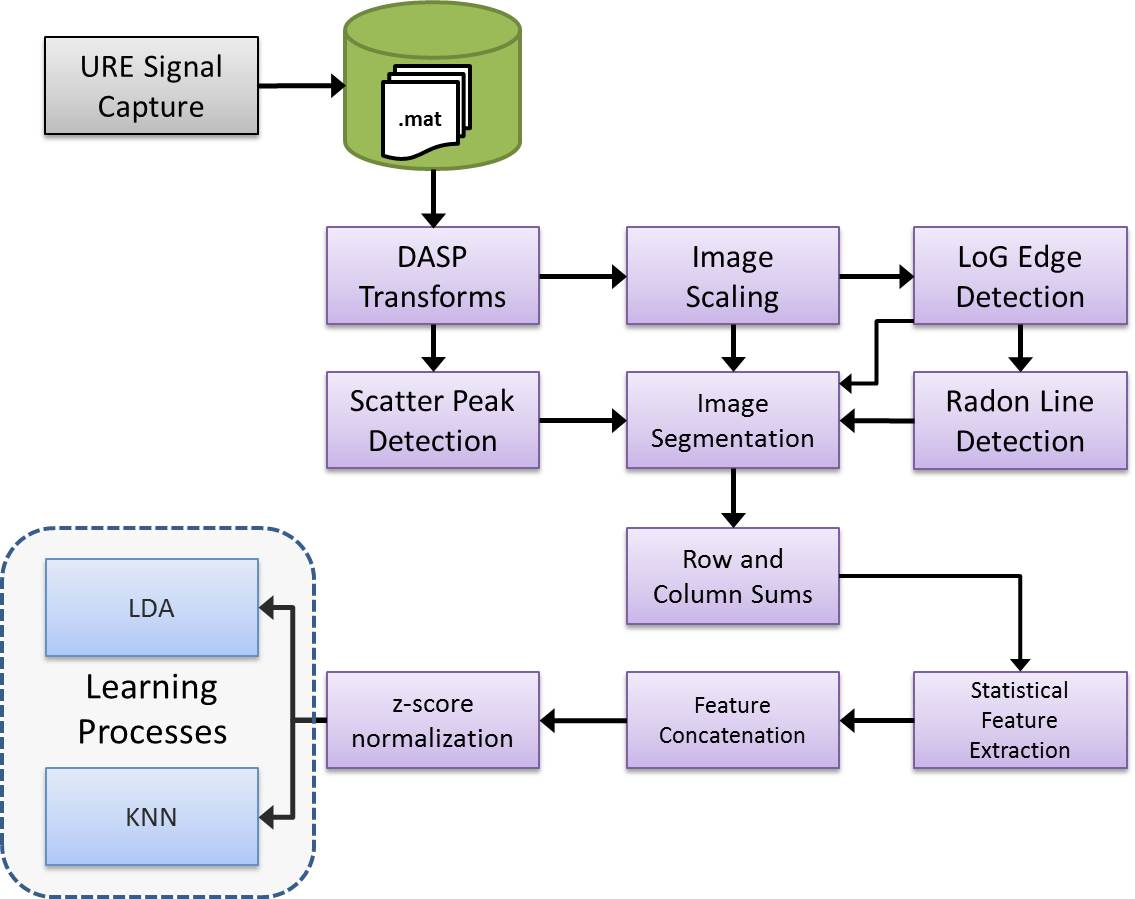
\includegraphics[width=\textwidth]{./misc_graphics/dasp_lda_knn_process_flow.jpg}
	\centering
	\caption{Flow diagram of the DASP processing flow from URE signal capture through the LDA and k-NN learning process.}
	\label{fig:dasp_lda_knn_process_flow}
\end{figure}
 
Figure \ref{fig:dasp_lda_knn_process_flow} outlines the DASP processing flow to generate feature vectors for LDA and k-NN testing and training.   All URE signal captures were initially processed through the DASP transforms with up to four images extracted from each DASP transform, the raw scaled image, the scatter peak detector image, the LoG edge detector image, and the radon line detector image.  Statistical feature vectors were then extracted from the DASP images by first segmenting the image and then performing row and column summing to obtain statistical sample vectors.  The statistical measurements were then concatenated in to a 1-D feature vector per sample and normalized by their z-score across all samples.  The normalized feature vectors were evaluated through the LDA and k-NN learning processes.

Figure \ref{fig:dasp_cnn_process_flow} provides an overview of the DASP processing flow for the CNN learning process.  Instead of image segmentation and feature vector extraction, the CNN learner only requires an image input for learning.  Similar to the feature vector processing flow, the CNN process generates up to four images for each DASP transform, the raw scaled image, the scatter peak detector image, the LoG edge detector image, and the radon line detector image.  The resulting DASP images were saved as individual Tag Image File Format (TIFF) files for cataloging, labeling, training, and testing with the CNN learner.

\begin{figure}[tb]
	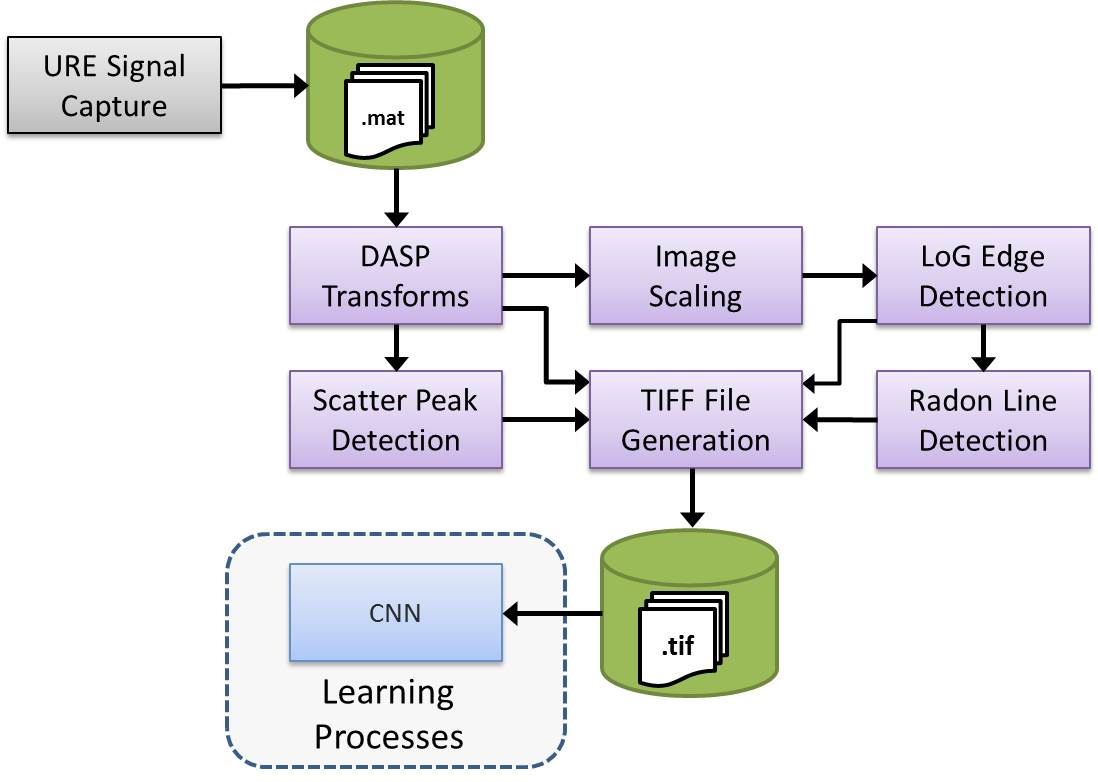
\includegraphics[width=\textwidth]{./misc_graphics/dasp_cnn_process_flow.jpg}
	\centering
	\caption{Flow diagram of the DASP processing flow from URE signal capture through the CNN learning process.}
	\label{fig:dasp_cnn_process_flow}
\end{figure}

\section[DASP Processes and Transforms]{DASP Processes and Transforms}

Because no \emph{a priori} knowledge of the test devices' URE characteristics were taken in to account in the DASP evaluation process, the DASP algorithms, transforms, and parameter settings were selected heuristically to include as much of the URE spectrum that could be reasonably achieved given a $2$MS/s collection system and a one second capture time per device sample.  Table \ref{tab:dasp_config_parameters} provides a listing of the DASP algorithms and transforms used in the feature and image generation processes, along with their respective parameter settings.  All DASP algorithms were evaluated, including the SCAP auto-covariance vector, $\bf{S}_F$, while it should also be noted that not all combinations of DASP algorithms and image processing transforms were utilized.  In addition, the SCAP auto-covariance vector was not utilized by the CNN learner because it does not result in a 2-D image. 

\begin{table}[tb]
	\caption{Table of all DASP algorithms and image transforms used for image generation and feature extraction.}
	\centering
		\begin{tabular}{cc|c}
		\hline
		DASP Algorithm & Image Transform & Configuration Parameters\\
		\hline
    CMASP & Array & $f_c = 10000$\\
		CMASP & Edge Array & $Bc = 9500$ \\
		CMASP & Radon Array & $f_m = 1000$ \\
		& & $B_m = 950$ \\
		\hline
		FASP & Array & $N = 1000$ \\
		\hline
		HASP-F & Array & $f_c = 1000$ \\
		HASP-F & Edge Array & $B = 1990$ \\
		HASP-F & Radon Array & \\
		\hline
		HASP-D & Array & $f_c = 1000$ \\
		& & $B = 1990$ \\
		\hline
		MASP (Low) & Array & $N = 10000$\\
		MASP (Low) & Edge Array & $p = 0.02$ \\
		MASP (Low) & Radon Array & \\
		MASP (Low) & Scatter Plot &\\
		\hline
		MASP (High) & Array & $N = 1000$ \\
		MASP (High) & Edge Array & $p = 0.02$ \\
		MASP (High) & Radon Array & \\
		MASP (High) & Scatter Plot & \\	
		\hline
		SCAP & Array & $f_c = 1000$ \\
		SCAP & Cross-Covariance Vector & $B = 1990$ \\
    \hline
		\end{tabular}
	\label{tab:dasp_config_parameters}
\end{table}

Table \ref{tab:dasp_config_parameters} provides the configuration parameters for each DASP algorithm, based upon their specific input requirements.  Two sets of MASP images were generated with different settings to characterize low and high frequency modulations, with the higher frequency MASP algorithm trading off modulation frequency resolution.  The Edge and Radon Arrays were not applied to the FASP, HASP-D, and SCAP images because the additional benefit was not obvious given the multitude of curved lines present in the HASP-D and SCAP images and the large number of vertical lines in a typical FASP image.

\section[Statistical Feature Extraction]{Statistical Feature Extraction}

Statistical features were extracted from the whole and $3 \times 3$ segmented DASP images in Table \ref{tab:dasp_config_parameters} using the whole image, the summed row vector, and the summed column vector.  The extracted features for each image segment were concatenated in to a single feature vector 
\begin{equation}
	\textit{\textbf{X}}_s= [\sigma^{2}_{\omega},  \gamma_{\omega},  \kappa_{\omega}, \sigma^{2}_{\rho},  \gamma_{\rho},  \kappa_{\rho}, \sigma^{2}_{\gamma},  \gamma_{\gamma},  \kappa_{\gamma}]
	\label{eq:featureeq}
\end{equation}
where $\omega$ are the whole segment features, $\rho$ are summed row features, and $\gamma$ are summed column features, resulting in $9$ features for each of the DASP image segments.  The SCAP auto-covariance vector only provides a single vector for feature extraction and therefore only yielded three features, $[\sigma^{2},  \gamma,  \kappa]$.  Finally, the z-score for each feature was calculated across all data sets resulting in a normalized feature set that was utilized for subsequent training and classification analysis.  The image segment feature vectors, $\textit{\textbf{X}}_s$, were then concatenated to form a full feature vector
\begin{equation}
	\textit{\textbf{X}}= [\textit{\textbf{X}}_1, \textit{\textbf{X}}_2, \ldots, \textit{\textbf{X}}_9, \textit{\textbf{X}}_{10}]
	\label{eq:featureeq_cat}
\end{equation}
for each DASP image, where $\textit{\textbf{X}}_1$ is the top image segment and $\textit{\textbf{X}}_2$ through $\textit{\textbf{X}}_{10}$ are the $9$ image segments comprised of the $3 \times 3$ grid segmentation.  The concatenation of the image segment feature vectors resulted in a total of $9 \times 10 = 90$ features per DASP image, except for the SCAP auto-covariance feature vector which only returned three features.

\section[DASP Image Store]{DASP Image Store}

The MATLAB\textsuperscript \textregistered ~~Convolutional Neural Network implementation, including supporting tools such as the \textit{imageDataStore} command, was designed to seamlessly catalog, label, train, and test on image files.  To simplify the CNN learning process, each DASP image was saved as a \textit{.tif} file using the process in Algorithm \ref{alg:tiffimalg}.  The TIFF image generation algorithm is identical to the image scaling algorithm, Algorithm \ref{alg:imscalealg}, with the addition of the $16$bit scaling, image resizing, and file saving steps.  Each TIFF file was stored in its own directory structure within a labeled folder for class indexing.

\begin{algorithm}
	\caption{TIFF Image Generation Algorithm} \label{alg:tiffimalg}
	\scriptsize
	\begin{algorithmic}[1]
		\Require~~
		\Statex $\mathbf{I}$ - Input Image
		\Statex $\mathbf{I_b}$ - Background Image
		\Ensure~~
		\Statex $\mathbf{I_s}$ - Saved TIFF Image
		\Statex
		\State $\mathbf{I_s} \gets \mathbf{I} - \mathbf{I_b}$ 
		\State $\mathbf{I_s} \leq 0 \gets 0$
		\State $\mathbf{I_s}  \gets $ STANDARD DEVIATION FILTER of $\mathbf{I_s}$
		\State $\mathbf{I_s} \gets \log{\mathbf{I_s}}$
		\State $\mathbf{I_s} \gets 2^{16} \times \frac{\mathbf{I_s} - \min{\mathbf{I_s}}}{\max{\mathbf{I_s}} - \min{\mathbf{I_s}}}$
		\State RESIZE $\mathbf{I_s}$ to $500 \times 500$
		\State SAVE $\mathbf{I_s}$ as $16$bit TIFF Image file
	\end{algorithmic}
\end{algorithm}

% To compile single chapters put a % symbol in front of "\comment" and "}%end of comment" below 
%    and take off the % symbol from "\end{document" at the bottom line. Undo before compiling
%    the complete thesis
%%Note: You can only use \section command, you are not allowed, per TTU Graduate School, use
%%\subsection command for ghigher level subheadings. At most level 2 subheadings are allowed.

\chapter{DASP Feature Classification and Results}
\label{DASP Device Classification Chapter}

\section[Learning Overview]{Learning Overview}

The DASP algorithms described in Chapter \ref{DASP Algorithm Development Chapter} were specifically developed to align, cluster, or otherwise group URE signal features in a 2-D image structure, with a goal of providing a method for the detection, characterization, and classification of devices based upon their conducted URE.  To ascertain the performance of the DASP algorithms, conducted URE was first collected from a variety of electronic devices, as outlined in Chapter \ref{URE Data Collection Chapter}, to provide a suitable data set for evaluation.  In Chapter \ref{DASP Feature Extraction Chapter} a suite of algorithms was developed to scale and highlight features of interest within DASP images and, in addition, a method for extracting statistical features was also presented.  A processing flow for feature generation was defined in Chapter \ref{Simulation and Testing Configuration} to enable 1-D feature vector evaluation through LDA and k-NN machine learners.  Finally, all DASP images were scaled and stored as TIFF image files to enable image classification through MATLAB\textsuperscript \textregistered 's CNN deep learning framework.

Before evaluation of the classification performance of the DASP derived features, an initial unsupervised clustering analysis was performed on the statistical based features in Section \ref{Device Clustering Analysis} to determine if the features were separable and to better understand and visualize the data.  The DASP algorithms were evaluated for their performance in a one-versus-all classification configuration using LDA and k-NN with statistical-based features and CNN with the stored TIFF images in Section \ref{Single Device Classification}.  Section \ref{Multiple Device Classification} provides an evaluation of the DASP transforms and associated learning algorithms applied to an all-versus-all classification configuration where multiple URE signals were present in the same capture.  Finally, Section \ref{Clutter Analysis} presents analysis of a trained CNN's ability to detect URE clutter and associate unknown devices with known devices based upon their URE signatures. 

\section[Statistical Feature Clustering Analysis]{Statistical Feature Clustering Analysis}
\label{Device Clustering Analysis}

An initial clustering analysis was performed on the statistical based feature vectors to confirm the separability of device classes.  The feature vector for each sample was formed by concatenating features from all image segments (including the whole image) of all DASP transforms.  In the process of forming the feature vectors it was found that the MASP-Low Scatter, MASP-Low Edge Array, MASP-Low Radon Array, and MASP-High Scatter based statistical feature vectors contained invalid values.  Upon further examination, the scaling process applied to these DASP transforms resulted in a large number of columns and rows with all zeros and therefore generated undefined statistical values.  After removal of the four ill-formed DASP transform statistical feature vectors, the concatenation of the remaining feature vectors resulted in a combined feature matrix, $\textit{\bf{X}}_C$, of $12000$ samples by $1173$ features.  The $12000$ samples were the result of $1200$ samples per device with $9$ devices plus the \textit{None} class.  The $1173$ features were comprised of $13 \times 90$ features for the remaining $13$ DASP transforms plus the $3$ SCAP auto-covariance statistical features.

A Principal Component Analysis (PCA) rank reduction was applied to $\textit{\bf{X}}_C$ to reduce the feature space down to $3$ features, $\textit{\bf{X}}_{C,3}$, to aid in visualization.  Figure \ref{fig:cluster_truth} provides a 2-D scatter plot of the rank reduced statistical feature matrix with the class values encoded in the scatter colors.  With only $2$ features shown it was evident that at least $4$ classes (\textit{fluorescentlights}, \textit{dellmonitor}, \textit{dellxps}, and \textit{hpzbook}) were highly separable from the remaining $6$ classes.

\begin{figure}[tb]
	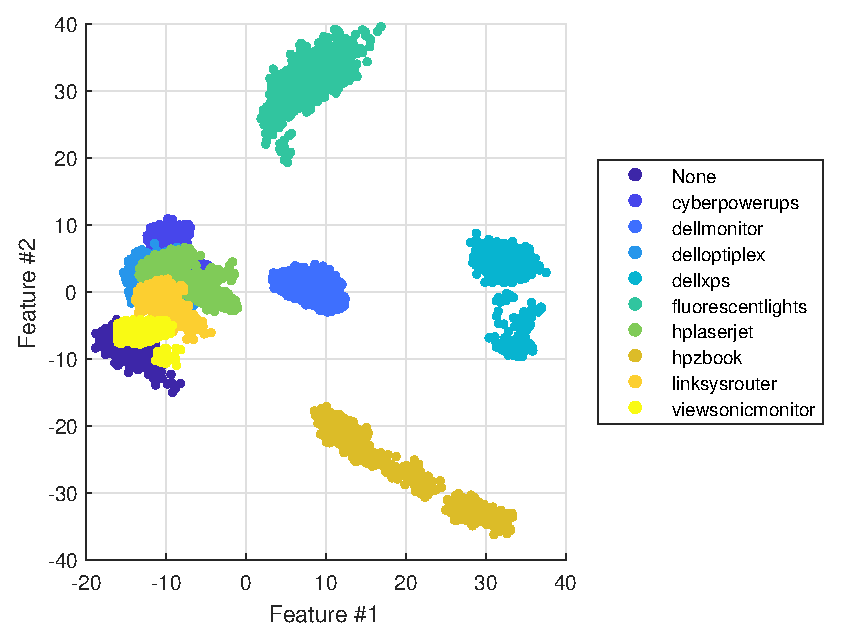
\includegraphics[width=\textwidth]{./dasp_algorithm_results/dasp_stat_cluster_truth.eps}
	\centering
	\caption{Scatter plot of the top two statistical features from the PCA reduced feature set.  The point colors represent the ground truth and show a clear separation among several of the classes (\textit{hpzbook}, \textit{dellxps}, \textit{fluorescentlights}, and \textit{dellmonitor}).}
	\label{fig:cluster_truth}
\end{figure}

Because only $4$ classes showed clear visual class separation through a 2-D projection of $\textit{\bf{X}}_{C,3}$, a gap analysis based upon a Gaussian-Mixture Model clustering was performed on the $\textit{\bf{X}}_{C,3}$ matrix to confirm the presence of approximately $10$ classes to further validate the data set.  Figure \ref{fig:cluster_gap} provides a plot of the gap values and corresponding standard deviations for $k = [1,2, \ldots, 19, 20]$\footnote{$k$ in the context of unsupervised clustering and k-means defines the number of classes (or clusters), as opposed to $k$ in the context of k-NN which corresponds to the number of nearest neighbors for supervised learning.}. 

\begin{figure}[tb]
	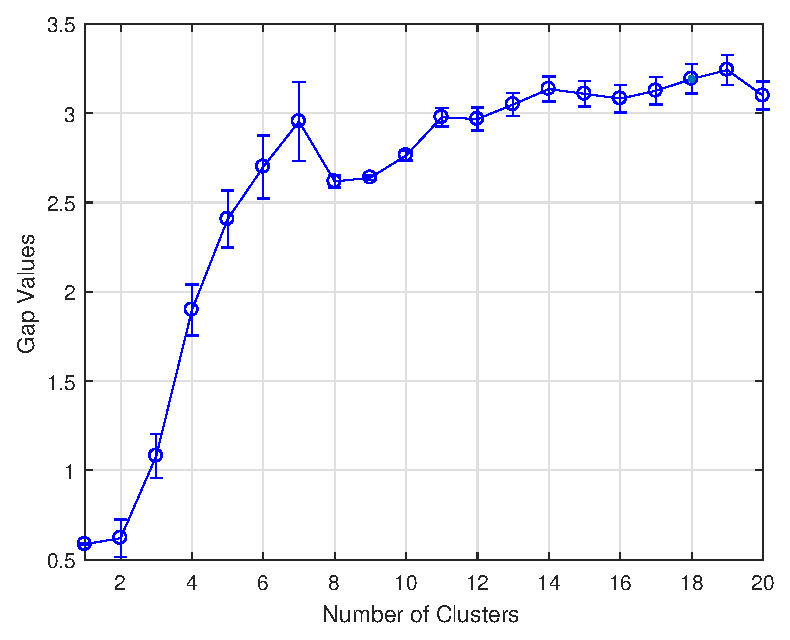
\includegraphics[width=\textwidth]{./dasp_algorithm_results/dasp_stat_cluster_gap.eps}
	\centering
	\caption{Plot of gap values with standard deviation error bars for the top three PCA reduced feature set, $\textit{\bf{X}}_{C,3}$.  The gap analysis shows a dip at $k=8$ with the minimum cluster variances between $k=8$ and $k=10$.}
	\label{fig:cluster_gap}
\end{figure}

Figure \ref{fig:cluster_gap} shows a dip in gap values at $k=8$ along with a corresponding drop in the standard deviation.  The minimum standard deviation occurs at $k=9$, with the second lowest standard deviation at $k=10$, which confirms the presence of approximately $8$ to $10$ classes.  Given that $k$ was known to be $10$, the gap assessment provided a good indicator that the statistical features were separable across all $10$ classes.  

A k-means clustering of the $\textit{\bf{X}}_{C,3}$ matrix with $k=10$ was then performed to further validate the results observed in the gap analysis, with the results shown in Figure \ref{fig:cluster_kmeans}.  The ``x'' marks show the k-means cluster centers, while the cluster colors are based upon a majority vote of known devices assigned to a particular cluster.  The k-means clustering did show many correct cluster assignments, however the \textit{hpzbook} cluster was incorrectly split in to two classes and the \textit{linksysrouter} class did not comprise the majority of any assigned cluster.

\begin{figure}[tb]
	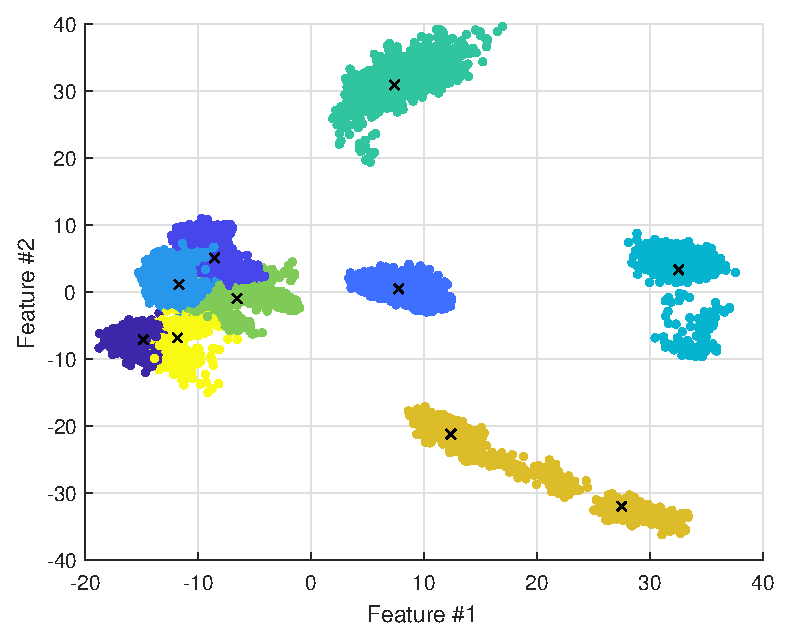
\includegraphics[width=\textwidth]{./dasp_algorithm_results/dasp_stat_cluster_kmeans.eps}
	\centering
	\caption{2-D scatter plot of a k-means clustering of top two statistical features from a PCA reduced feature set, with the ``x'' marks designating the k-means cluster centers.  The color coding and class assignments were based upon a majority vote of the known classes for a particular k-means cluster.  The k-means algorithm was not able to separate the \textit{linksysrouter} class from the overlapping clusters and incorrectly separated the \textit{hpzbook} class in to two separate clusters.}
	\label{fig:cluster_kmeans}
\end{figure}

Given the two distinct clusterings associated with the \textit{hpzbook} class, the k-means algorithm incorrectly separated the \textit{hpzbook} class and was therefore not able to generate a separate cluster with a majority of \textit{linksysrouter} devices.  The unsupervised clustering analysis showed that with only $3$ features the devices were mostly separable and indicated that a larger feature space may be required to correctly identify devices using supervised learning techniques.

\section[One-Versus-All Device Classification]{One-Versus-All Device Classification}
\label{Single Device Classification}

The DASP algorithms were first evaluated on their respective abilities to generate features relevant for one-versus-all classification.  Single device classification was performed based on the assumption that only one of the $10$ devices (or classes) was represented within a given sample.  One-versus-all classification was performed with LDA and k-NN learners on the statistical features as described in Section \ref{Statistical Features Single Device Classification}, whereas CNN learners were trained and tested against DASP images in a one-versus-all configuration as shown in Section \ref{Convolutional Neural Network Single Device Classification}.

\subsection[Statistical Feature Analysis]{Statistical Feature Analysis}
\label{Statistical Features Single Device Classification}

Before ascertaining the performance of the DASP-derived statistical features, several machine learning algorithms were evaluated based upon the following criteria:

\begin{itemize}
  \item Ability to provide one-versus-all multi-class classification results.
  \item Minimal or no “tuning” parameters.
	\item No prior knowledge of the class means or covariances.
	\item Robust and repeatable results.
	\item No requirement for an overly complex or optimum classifier.
	\item Retain some tie to the physical understanding of the underlying feature space.
	\item No requirement to handle class skew.
\end{itemize}
\label{list:ml_eval}

Several learning methods were explored for their applicability in evaluating the DASP statistical features, to include LDA, QDA, k-NN, Perceptrons, AdaBoost, and neural networks.  Although many of the candidate learning algorithms could have provided nearly optimum results in terms of classification, an optimized learner was not necessarily required for evaluation of the DASP-derived features.  Given the self-imposed requirements for the machine learning algorithm, neural networks and AdaBoost were eliminated based upon their high level of abstraction between the feature space and the learner, tuning parameter sensitivity, and repeatability \cite{Friedman2001}. 

The remaining algorithms, LDA, QDA, k-NN, and Perceptrons were further evaluated with LDA and k-NN eventually being utilized. Perceptrons may not converge or can take a long time to converge if the classes are not linearly separable and, in addition, the decision plane may change given different starting conditions \cite{Friedman2001}. LDA and QDA are closely related and differ only in the underlying assumption in the equality of class covariances with both providing similar classification performance.  LDA was eventually chosen for its simplicity, repeatability, and direct physical tie to the feature space where it attempts to maximize the distance between the class means and minimize the within-class variance \cite{Friedman2001}.  Certain assumptions were made about the underlying feature space for LDA to be a valid choice for classification.  LDA assumes that the feature means and variances are Gaussian distributed and each class shares the same covariance.  Furthermore, the utilization of LDA assumes that the classes are linearly separable. 

To balance the closed-form statistical-based solutions provided by LDA, k-NN was also used as an secondary learning method because of its non-parametric approach and simplicity.  In addition, k-NN does not make any assumptions about the underlying data such as linear separability and the equality of class covariances.  Although the choice of classifiers would have been re-evaluated had the early classification attempts performed poorly, LDA and k-NN were able to separate DASP generated statistical features at high classification accuracies ($>90\%$) in early testing and provided a robust and repeatable evaluation method for comparing the various DASP algorithms.

Table \ref{tab:stat_lda_acc} provides the results of a $4$-fold one-versus-all LDA classifier applied to the statistical-based DASP features for each of the $14$ DASP algorithm and image transform combinations as outlined in Table \ref{tab:dasp_config_parameters}, excluding the MASP-Low Scatter, MASP-Low Edge Array, MASP-Low Radon Array, and MASP-High Scatter combinations because of their previously noted invalid feature vectors.  Each DASP combination was evaluated using the entire feature set across all segments, $\textit{\bf{X}}$, using only the top image segment, $\textit{\bf{X}}_1$, and using a rank $3$ PCA reduced feature set.  The ``Combined'' DASP feature set, $\textit{\bf{X}}_C$, was formed by concatenating the $\textit{\bf{X}}$ feature vectors for all valid DASP algorithm and transform combinations.

\begin{table}[tb]
	\caption{One-versus-all 4-fold cross validation LDA classification accuracies for the statistically derived features.  All algorithms (except the SCAP-vec feature set) exceeded $95\%$ accuracy when all segments were used, while the majority still exceeded $82\%$ when only the top grid was leveraged.  }
	\csvautotabular{./dasp_algorithm_results/dasp_stat_lda_results.txt}
	\centering
	\label{tab:stat_lda_acc}
\end{table}

The results in Table \ref{tab:stat_lda_acc} show that using all segments, or $90$ features, provided accuracies exceeding $98\%$ for the majority of DASP combinations.  Using only $9$ features from the top segment provided accuracies on the order of $85\%$, with HASP-F Radon Array providing the highest accuracy at $94.7\%$.  The reduced rank feature sets performed worse, on average, than the $\textit{\bf{X}}$ and $\textit{\bf{X}}_1$ feature sets, however the rank reduced Combined feature set, $\textit{\bf{X}}_{C,3}$, was able to obtain an accuracy of $94.6\%$ with only $3$ features.  It should be noted that the although the combination of all segments and all feature sets, $\textit{\bf{X}}_C$, was able to reach an accuracy of $100\%$, it utilized a feature vector length of $1173$, or greater than $10$ times the number of features in the individual DASP combinations.

Table \ref{tab:stat_knn_acc} provides the results of a $4$-fold one-versus-all k-NN classifier applied to the statistical-based DASP features for each of the $14$ DASP algorithm and image transform combinations as outlined in Table \ref{tab:dasp_config_parameters}, excluding the MASP-Low Scatter, MASP-Low Edge Array, MASP-Low Radon Array, and MASP-High Scatter combinations.  The k-NN learner was configured to utilize an inverse-squared Euclidean distance metric with $k=10$ nearest neighbors.  Each DASP combination was evaluated using the entire feature set from all segments, $\textit{\bf{X}}$, only the top image segment, $\textit{\bf{X}}_1$, and using a rank $3$ PCA reduced feature set.  

\begin{table}[tb]
	\caption{One-versus-all 4-fold cross validation k-NN classification accuracies for the statistically derived features for all DASP algorithm and image transformations.  All algorithms (except the SCAP-vec feature set) exceeded $95\%$ accuracy when all grids were used, while the majority were in the $80\%$ range when only the top grid was leveraged.  Several of the PCA rank reduced feature sets exceeded $90\%$ with the combined feature set obtaining $96.7\%$, while the majority were in the $80\%$ range.}
	\csvautotabular{./dasp_algorithm_results/dasp_stat_knn_results.txt}
	\centering
	\label{tab:stat_knn_acc}
\end{table}

The results in Table \ref{tab:stat_knn_acc} show that using $\textit{\bf{X}}$, or $90$ features, provided accuracies exceeding $98\%$ for the majority of DASP combinations with the HASP-F Array, HASP-D Array, and Combined feature sets reaching $100\%$.  Using only $9$ features from the top segment, $\textit{\bf{X}}_1$, provided accuracies on the order of $95\%$, with the SCAP Array features providing the highest accuracy at $97.2\%$.  The reduced rank feature sets performed only slightly worse on average than the $\textit{\bf{X}}$ and $\textit{\bf{X}}_1$ feature sets, however the rank reduced Combined feature set, $\textit{\bf{X}}_{C,3}$, was able to obtain an accuracy of $97.2\%$, while the HASP-D Array, HASP-F Array, and FASP Array features sets also exceeded $90\%$ with only $3$ features.  As with the LDA results, it should be noted that although the $\textit{\bf{X}}_C$ feature set was able to reach an accuracy of $100\%$, it utilized a feature vector length of $1173$, or greater the $10$ times the number of features in the individual DASP combinations. 

The k-NN learning algorithm significantly outperformed the LDA learning method, especially with the Top segment and rank reduced feature sets indicating that the assumptions underlying the LDA algorithm, such as linear separability and Gaussian distribution of features, were not valid.  Figure \ref{fig:stat_cm_cum} provides a cumulative confusion matrix generated by averaging all of the confusion matrices of the LDA and k-NN learners.   

\begin{figure}[tb]
	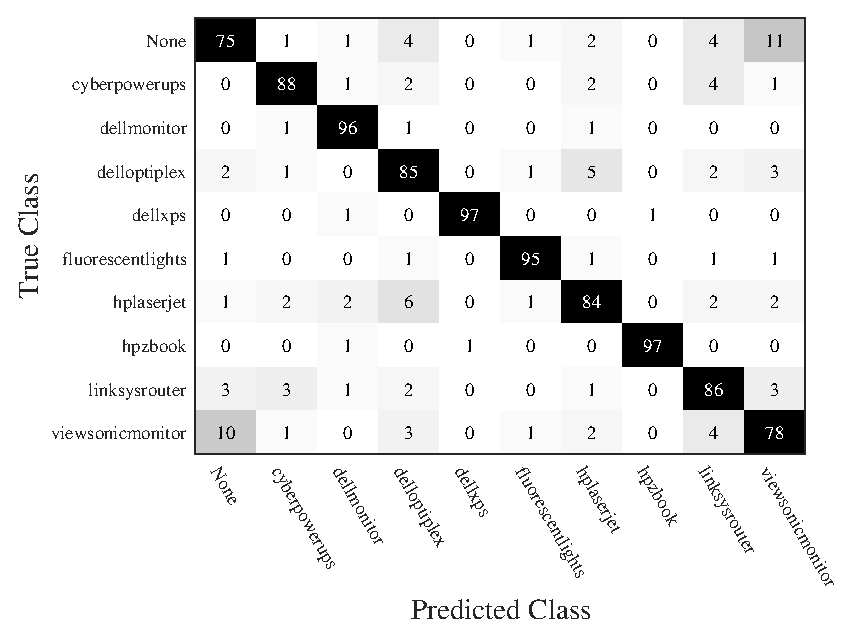
\includegraphics[width=\textwidth]{./dasp_algorithm_results/dasp_stat_AllCombined_conf.eps}
	\centering
	\caption{Cumulative confusion matrix for all of the results in Table \ref{tab:stat_lda_acc} and Table \ref{tab:stat_knn_acc}.  Results were obtained by summing the confusion matrices of all LDA and k-NN results and normalizing to percentages.  The table shows that the majority of the classes performed well with no strong confusion between two classes except for the \textit{viewsonicmonitor} class which was confused with the \textit{None} class at a rate of $11\%$.}
	\label{fig:stat_cm_cum}
\end{figure}

The cumulative results show that the largest confusion existed between the \textit{viewsonicmonitor} and \textit{None} devices with an $11\%$ misclassification rate.  The second highest misclassification rate of $6\%$ occurred between the \textit{delloptiplex} and \textit{hplaserjet} devices.  Interestingly, Figure \ref{fig:cluster_truth} shows significant overlap between the \textit{viewsonicmonitor} and \textit{None} classes and the \textit{delloptiplex} and \textit{hplaserjet} classes in the 2-D scatter plot of $\textit{\bf{X}}_{C,3}$, thus providing results consistent with Figure \ref{fig:stat_cm_cum}.

\subsection[DASP Image Analysis]{DASP Image Analysis}
\label{Convolutional Neural Network Single Device Classification}

Convolutional Neural Networks are a deep learning framework specifically designed for processing and classifying images and are widely used in the object recognition and computer vision communities.  CNNs have a variety of building blocks with an infinite number of configurations, but the foundational component of a CNN is the convolution (conv) layer.  The convolution layer is comprised of tunable filters that are updated through training to highlight areas, objects, or features within an image.  Convolution layers are typically followed by an activation layer and a pooling (pool) layer that ``scan'' and ``downsample'' the convolution filter outputs.  The pooling layer can ``downsample'' by several different methods, such as maximum pooling or averaging pooling, as it ``scans'' the convolution filter output by a fixed stride length.  The rectifying linear unit (reLU) implements the function $f(x) = \max(0,x)$ and is typically used as the activation layer.  A fully connected (fc) layer is implemented to connect with all input neurons and provide a scaled output by adding a bias and multiplying by a weighting factor.  The fully connected layer provides the higher level learning by calculating the appropriate convolution and pooling layer input weights for classification.   For instance, a series of convolution, activation, and pooling layers may learn an ``eye'', a ``nose'', and a ``mouth'', but the fully connected layer learns that together these features form a ``face''. 

As opposed to learning on feature vectors, as demonstrated in Section \ref{Statistical Features Single Device Classification}, a CNN trains and learns directly from the DASP images.  A very basic CNN was developed to perform one-versus-all classification of the DASP images, as described in Figure \ref{fig:cnn_net_single}.  The network consisted of an initial single-channel image input layer which resized the $500 \times 500$ pixel TIFF images to $25 \times 25$ pixels.  The input layer was followed by a convolution layer (\textit{conv1}) comprised of $20$ filters of size $5 \times 5$, a reLU layer, a max pooling layer (\textit{pool1}) with a $2 \times 2$ downsampling filter and a stride of $2$.  A fully connected layer (\textit{fc1}) with $10$ output neurons was utilized for the higher level learning.  A softmax classification layer was used to perform the one-versus-all classification.

\begin{figure}[htbp!]
	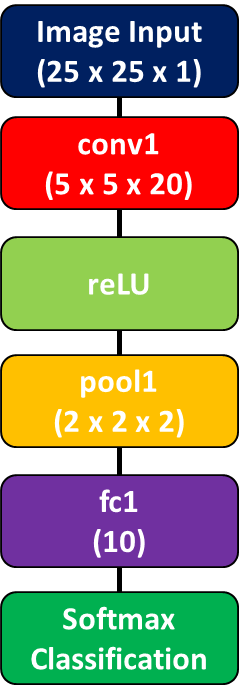
\includegraphics[width=0.3\textwidth,keepaspectratio]{./misc_graphics/dasp_cnn_simple_network.png}
	\centering
	\caption{Diagram of the Convolutional Neural Network used for one versus all device classification of DASP images. The network only utilizes one convolution, max pooling, and fully connected layer, in addition to a $25 \times 25$ image input layer.}
	\label{fig:cnn_net_single}
\end{figure}

The CNN in Figure \ref{fig:cnn_net_single} was trained using the parameters in Table \ref{tab:cnn_simple_train} where the Stochastic Gradient Descent with Momentum (SGDM) is defined by \footnote{https://www.mathworks.com/help/nnet/ref/trainingoptions.html, June $23$, $2017$}
\begin{equation}
    \theta_{l+1} = \theta_{l} - \alpha \nabla E \left(\theta_{l}\right) + \gamma \left( \theta_{l} - \theta_{l-1} \right)
		\label{eq:sgdmeq}
\end{equation}
where $l$ is the iteration number, $\alpha$ is the learning rate, $\theta$ specifies the updated parameter, and $E(\theta)$ is the cross entropy loss function
\begin{equation}
    E(\theta) = \sum^{n}_{i=1} \sum^{k}_{j=1} t_{ij} \ln y_{j} \left( x_{i},\theta \right)
		\label{eq:xentropyeq}
\end{equation}
 where $t_{ij}$ indicates the $i^{th}$ sample number is a member of the $j^{th}$ class and $y_{j}(x_{i},\theta)$ is the output for the $i^{th}$ sample.

\begin{table}[tb]
	\caption{Table of training parameters for the one-versus-all CNN.}
	\centering
		\begin{tabular}{c|c}
		\hline
		CNN Training Parameter & Parameter Value\\
		\hline
    Test Image Holdback Percentage & $20\%$ \\
		Learning Rate &  $1\times10^{-6}$\\
		Mini-Batch Size & $150$ \\
		Loss Function & Cross Entropy Function\\
		Update Algorithm & Stochastic Gradient Descent with Momentum\\
    \hline
		\end{tabular}
	\label{tab:cnn_simple_train}
\end{table}

Table \ref{tab:cnn_single_results} provides the blind testing results of the trained one-versus-all CNN.  All DASP image and transform combinations provided a greater than $97\%$ accuracy, with the SCAP Array being the best performer at $99.9\%$.  The MATLAB\textsuperscript \textregistered~CNN architecture does not allow for multiple column convolution streams\footnote{as of June, $2017$} so combined training on all DASP image combinations could not be implemented, but given the near optimal results from the individual DASP image transforms the combined training and testing was not required for the one-versus-all device classification.  

\begin{table}[tb]
	\caption{One-versus-all CNN classification results for all DASP algorithm processes.  All processes attained a greater than $97\%$ classification accuracy, with $10$ achieving accuracies greater than $99\%$.}
	\csvautotabular{./dasp_algorithm_results/dasp_cnn_results.txt}
	\centering
	\label{tab:cnn_single_results}
\end{table}

MATLAB\textsuperscript \textregistered ~ provides a method for inspecting a trained CNN network through the \textit{deepDreamImage} \footnote{https://www.mathworks.com/help/nnet/ref/deepdreamimage.html, July $06$, $2017$} command.  DeepDream image creation was developed by Google\textsuperscript \textregistered ~~ \cite{Mordvintsev2015} to allow researchers to visualize a composite image of layer activations within a trained network to develop understanding and insights into the learned features from a given training set.  Table \ref{tab:cnn_fc_dream_table} shows the \textit{deepDreamImage} outputs for the fully connected layers of select trained CNNs.  The DeepDream images looked very similar in structure to the DASP training images illustrated in Chapter \ref{DASP Algorithm Development Chapter} and Appendix B.  Appendix B provides sample images of all DASP transformations for all test and training devices in Table \ref{tab:collection_devices}.  The CMASP Edge Array DeepDream image, Figure \ref{fig:cnnfc2}, is particularly interesting in that a checkerboard pattern was formed to process the large number of intersecting lines and radials that are inherent to CMASP images.

{\centering
\begin{table}[tb]
	\caption{Table of DeepDream images of select fully connected layers from the one-versus-all CNNs trained on DASP images.  The DeepDream images highlight the learned activations associated with the DASP training images.}
	\begin{tabular}{ccc}
		\begin{subfigure}{0.3\textwidth}\centering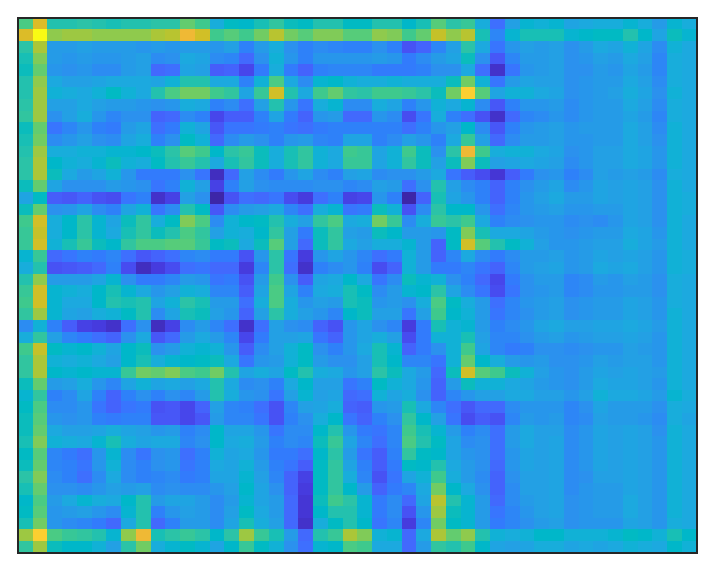
\includegraphics[width=0.8\columnwidth]{./dasp_algorithm_results/dasp_cnn_single_dream_fc_2.eps}
		\caption{CMASP, Edge Array}\label{fig:cnnfc2}
		\end{subfigure}&
		\begin{subfigure}{0.3\textwidth}\centering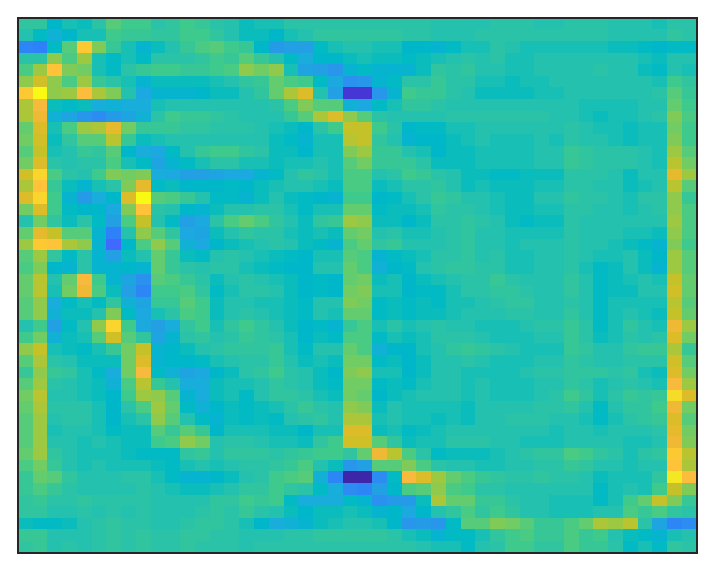
\includegraphics[width=0.8\columnwidth]{./dasp_algorithm_results/dasp_cnn_single_dream_fc_3.eps}
		\caption{CMASP, Radon Array}\label{fig:cnnfc3}
		\end{subfigure}&
		\begin{subfigure}{0.3\textwidth}\centering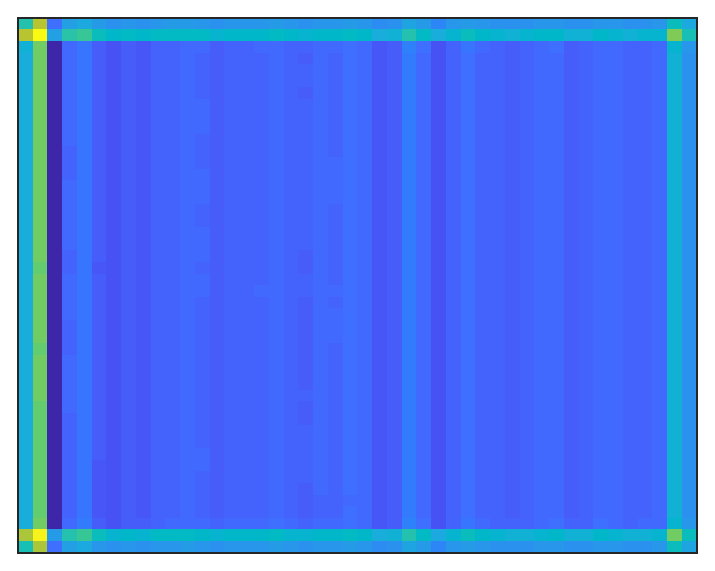
\includegraphics[width=0.8\columnwidth]{./dasp_algorithm_results/dasp_cnn_single_dream_fc_4.eps}
		\caption{FASP, Array}\label{fig:cnnfc4}
		\end{subfigure}    \\
		\begin{subfigure}{0.3\textwidth}\centering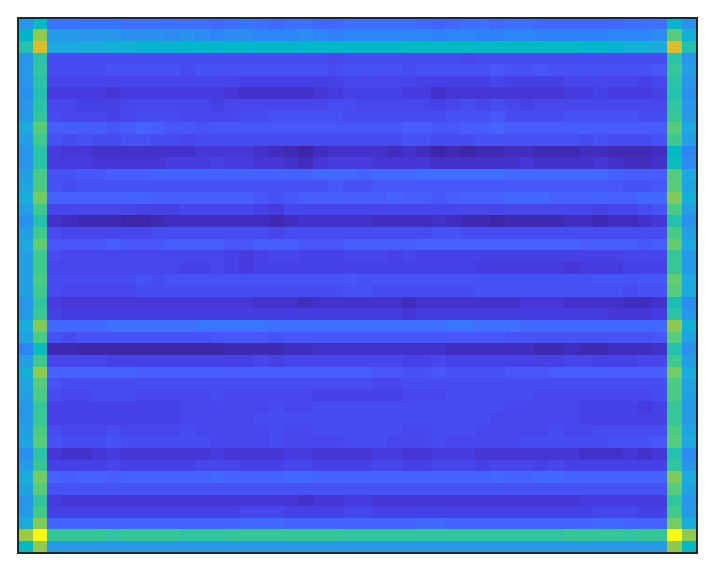
\includegraphics[width=0.8\columnwidth]{./dasp_algorithm_results/dasp_cnn_single_dream_fc_6.eps}
		\caption{HASP-F, Edge Array}\label{fig:cnnfc6}
		\end{subfigure}&
		\begin{subfigure}{0.3\textwidth}\centering\includegraphics[width=0.8\columnwidth]{./dasp_algorithm_results/dasp_cnn_single_dream_fc_7.eps}
		\caption{HASP-F, Radon Array}\label{fig:cnnfc7}
		\end{subfigure}&
		\begin{subfigure}{0.3\textwidth}\centering\includegraphics[width=0.8\columnwidth]{./dasp_algorithm_results/dasp_cnn_single_dream_fc_8.eps}
		\caption{HASP-D, Array}\label{fig:cnnfc8}
		\end{subfigure}    \\
		\begin{subfigure}{0.3\textwidth}\centering\includegraphics[width=0.8\columnwidth]{./dasp_algorithm_results/dasp_cnn_single_dream_fc_9.eps}
		\caption{MASP (Low), Array}\label{fig:cnnfc9}
		\end{subfigure}&
		\begin{subfigure}{0.3\textwidth}\centering\includegraphics[width=0.8\columnwidth]{./dasp_algorithm_results/dasp_cnn_single_dream_fc_10.eps}
		\caption{MASP (Low), Scatter}\label{fig:cnnfc10}
		\end{subfigure}&
		\begin{subfigure}{0.3\textwidth}\centering\includegraphics[width=0.8\columnwidth]{./dasp_algorithm_results/dasp_cnn_single_dream_fc_11.eps}
		\caption{MASP (Low), Edge Array}\label{fig:cnnfc11}
		\end{subfigure}    \\
		\begin{subfigure}{0.3\textwidth}\centering\includegraphics[width=0.8\columnwidth]{./dasp_algorithm_results/dasp_cnn_single_dream_fc_13.eps}
		\caption{MASP (High), Array}\label{fig:cnnfc13}
		\end{subfigure}&
		\begin{subfigure}{0.3\textwidth}\centering\includegraphics[width=0.8\columnwidth]{./dasp_algorithm_results/dasp_cnn_single_dream_fc_14.eps}
		\caption{MASP (High), Scatter}\label{fig:cnnfc14}
		\end{subfigure}&
		\begin{subfigure}{0.3\textwidth}\centering\includegraphics[width=0.8\columnwidth]{./dasp_algorithm_results/dasp_cnn_single_dream_fc_17.eps}
		\caption{SCAP, Array}\label{fig:cnnfc17}
		\end{subfigure}
	\end{tabular}
\label{tab:cnn_fc_dream_table}
\end{table}
}

\section[Multiple Device Classification]{Multiple Device Classification}
\label{Multiple Device Classification}

One-versus-all classification analysis in Section \ref{Single Device Classification} assumed that one and only one device was present in a given URE capture; however, that is not completely practical in an environment where many devices may be operating at the same time.  The LDA, k-NN, and CNN learners were all designed for one-versus-all classification and therefore were adapted for all-versus-all classification.  There are several methods for accomplishing multi-device detection and classification, 1) train a multi-class classifier for one-versus-all classification and set a threshold for detection, 2) train separate two-class classifiers for each device in a one-versus-none testing configuration, or 3) train a multi-class classifier with multiple labels per sample.  LDA cannot be trained as an all-versus-all multi-class classifier and therefore could not be easily adapted other than to develop a threshold for detection of present devices.  CNNs can be trained with multiple labels per sample given an appropriate network and loss function, however MATLAB\textsuperscript \textregistered ~ does not provide this functionality and therefore the CNN's previously trained on single-devices were adapted, similarly to the LDA learner, with a threshold to detect multiple classes.  \cite{Sorower2010, Zhang2007, Spyromitros2008} demonstrate the feasibility of using k-NN learners for multi-label classification, with the majority of the multi-label k-NN learners being adaptations of one-versus-none learning (Binary Relevance).  Given the threshold based approach of the LDA and CNN learners, the one-versus-all training of the LDA and CNN learners, and the redundancy in analyzing the statistical-based feature sets with k-NN, a multi-label k-NN was not utilized for processing of the multi-device statistical feature vectors. 

\subsection[Multiple Device Test Configuration]{Multiple Device Test Configuration}

Multi-device capture files were generated to test the single device trained LDA and CNN learners for multi-device classification.  The URE collection effort outlined in Chapter \ref{URE Data Collection Chapter} only collected a single device per capture, therefore single device captures were added in the time domain to form multi-device URE files.  One hundred multi-device captures were generated for each of $2$ through $9$ device combinations.  The multi-device combinations files were generated through a random selection process that excluded the \textit{None} state and more than one example of a class within a given multi-device file.  The multi-file generation process therefore generated $(9-2) \times 100 = 700$ multi-device test files.

The multi-device time domain files were subsequently processed with the DASP algorithms, feature extractors, and TIFF image creation processes outlined in Figure \ref{fig:dasp_lda_knn_process_flow} and Figure \ref{fig:dasp_cnn_process_flow}.  The generated multi-device DASP arrays and files were not used for training, but only as test inputs to the LDA and CNN learners trained on single devices.  To illustrate the superposition of multiple devices within a DASP image Figure \ref{fig:multi_device_image} shows the individual MASP (Low) scatter images for the \textit{cyberpowerups} and \textit{fluorescentlights}, as well as the combined MASP (Low) scatter image derived from the URE time domain superpositioning of the two devices.  The combined image shows artifacts of both the \textit{cyberpowerups} and \textit{fluorescentlights} device images as highlighted by the oval and circle, respectively.   

\begin{figure}[htbp!]
	\includegraphics[width=\textwidth,height=\textheight,keepaspectratio]{./misc_graphics/multiDeivceImages.png}
	\centering
	\caption{MASP (Low) Scatter images for the \textit{cyberpowerups}, \textit{fluorescentlights}, and the multi-device combined image.  DASP image features for the \textit{cyberpowerups} and \textit{fluorescentlights} devices are shown by the oval and round circles, respectively.}
	\label{fig:multi_device_image}
\end{figure}

\subsection[Statistical Feature Analysis]{Statistical Feature Analysis}
\label{Statistical Features Multiple Device Classification}

The LDA learner trained in a one-versus-all method calculates a ``score'' for each class and selects the class with the greatest score.  To adapt for multi-device classification, the score vector was normalized using their z-score and a threshold of $0.5$ standard deviations was utilized to detect the presence of a specific class.  The results of the multi-device LDA classifier are shown in Table \ref{tab:stat_lda_multi} for each of the DASP combinations, including the results of the combined feature set.  The accuracy (ACC), true positive rate (TPR), false positive rate (FPR) true negative rate (TNR), false negative rate (FNR), precision (PR), and F-score (FSCORE) are provided. 

\begin{table}[tb]
	\caption{Classification accuracies and statistical measures of the multi-class LDA classifier using statistical based feature sets derived from all DASP algorithm processes.  Given $9$ possible class assignments with the \textit{None} class removed, the overall accuracies were around $50\%$.   Although the classifiers had significant False Negative Rates, the majority had Precisions exceeding $75\%$.  The MASP (High) Array feature set performed best with a precision of $1$, while only providing an accuracy of $50.9\%$ and a True Positive Rate of $0.2$.}
	\csvautotabular{./dasp_algorithm_results/dasp_stat_lda_all_multi_results.txt}
	\centering

	\label{tab:stat_lda_multi}
\end{table}

The results in Table \ref{tab:stat_lda_multi} show poor accuracy for all DASP combinations, however the false positive rates were relatively low which is further reflected in the high precisions, with the MASP (High) Array and Combined feature sets attaining precisions of $1$ and $0.96$, respectively.  Further analysis showed that the learners also had a high rate of false negatives, which taken in combination with the high precisions, means that while the LDA learners often missed the presence of a device they were detected with high confidence.  It should also be noted that the multi-device LDA learner was not trained on the \textit{None} state.  The assumption was made that the presence of a device was already determined and therefore the multi-device classifier was utilized to determine if a specific known device was present.

\subsection[DASP Image Analysis]{DASP Image Analysis}
\label{Convolutional Neural Network Multiple Device Classification}

The process of using a CNN learner trained on single devices to test for the presence of multiple device was handled in much the same way as that of the LDA learner in Section \ref{Statistical Features Multiple Device Classification}.  A score vector was extracted from the CNN network for each test sample and scaled by their z-score.  A threshold of $0.5$ standard deviations was then used to detect the presence of a given device.  To combine the DASP algorithms, the pre-normalized score vectors for each of the DASP algorithms were summed together, normalized, then compared to the detection threshold.  Early testing using the very basic CNN described in Figure \ref{fig:cnn_net_single}, showed very poor results due to network simplicity and over-training and, therefore, a new CNN was designed to better address multi-device classification and prevent over-training.

Figure \ref{fig:cnn_net_multi} shows the network topology of the multi-device CNN with reduced over-training susceptibility and improved multi-device classification performance.  The network used a single-channel image input layer that resizes input images to $100 \times 100$ pixels, as opposed to the $25 \times 25$ resolution in the single device CNN.  The input was connected to a $20\%$ dropout layer which was followed by two serially connected sets of convolution, reLU, max-pooling layers.  The dropout layer at the input sets each of its $100 \times 100$ pixel inputs to zero with a probability of $20\%$ to limit over-training of the network \cite{Srivastava2014}.  The two convolution layers, \textit{conv1} and \textit{conv2}, were each configured with $10$ filters of sizes $10 \times 10$ and $5 \times 5$, respectively. Both of the max-pooling layers utilized a $2 \times 2$ downsampling filter with a stride of one.  A fully connected layer (\textit{fc1}) with an output width of $100$ followed the convolution and pooling layers and feeds an additional reLU layer and $50\%$ dropout layer.  A final fully connected layer (\textit{fc2}) with an output width of $10$ was then followed by the softmax classification layer.  The dropout layers were added to specifically prevent, or at least limit, over training of the more complex network.  The additional convolution pooling layers were added to allow for processing of more complex shapes and structures within the DASP images, while the additional $100$ wide fully connected layer was included for higher levels of learning and abstraction.

\begin{figure}[htbp!]
	\includegraphics[width=0.2\textwidth,keepaspectratio]{./misc_graphics/dasp_cnn_multi_network.png}
	\centering
	\caption{Diagram of the Convolutional Neural Network used for multi-class device classification of DASP images. The input layer compressed input images to $100 \times 100$pixels, while only utilizing two convolution, max pooling, and fully connected layers along with two dropout layers to limit over training.  A fully connected layer of width $100$ was included to allow for higher level learning.}
	\label{fig:cnn_net_multi}
\end{figure}

The results from the multi-device testing of the trained multi-class CNNs are presented in Table \ref{tab:cnn_multi_testrmvd}.  The results for all $17$ of the DASP image and transform combinations is shown along with the combined CNN learner results.  Although the CNNs did not provide great accuracies, averaging slightly under $60\%$, they did outperform the LDA multi-device classifiers and were able to achieve a high average precision of $88\%$ with the combined results attaining a precision of $97\%$.  As with the LDA results, the CNN multi-device classifiers had high false negative rates, but reported the presence of devices with high confidence.

\begin{table}[tb]
	\caption{Classification accuracies and statistical metrics of the CNN multi-class classifiers.  The classification accuracies averaged around $60\%$, while classification Precisions were on the order of $0.90$. The combined CNN learner obtained an accuracy of $66.7\%$ and a $0.97$ precision.}
	\csvautotabular{./dasp_algorithm_results/dasp_cnn_multi_nonemultirmvd_results.txt}
	\centering
	\label{tab:cnn_multi_testrmvd}
\end{table}
 
Table \ref{tab:cnn_multi_acc_add_device} provides a listing of CNN multi-device classification results versus the number of devices present within a given test sample.  Initial inspection showed a monotonically decreasing accuracy which was to be expected in that more devices would result in more noise and signal confounders to contribute to misclassification, but for captures with less than $5$ devices accuracies exceeded $79\%$ with precisions exceeding $83\%$.  It should be noted that for $9$ devices in a given capture, there can be no false positives or true negatives in that all classes are present.  

\begin{table}[tb]
	\caption{Classification accuracies and statistical metrics of the CNN multi-class classifiers with respect to the number of devices within the test capture.  The relative accuracies monotonically decreased for each additional device, validating the testing approach.  The precisions monotonically increased ultimately reaching $1$ at $9$ devices, which was expected because all devices are present and any detected device was by definition the correct answer.}
	\csvautotabular{./dasp_algorithm_results/dasp_cnn_multi_nonemultirmvd_results_versus_numdevices.txt}
	\centering
	\label{tab:cnn_multi_acc_add_device}
\end{table}

In addition to analyzing the multi-class results based on the number of devices, an analysis was also performed to evaluate the classifier performance based upon the presence of a particular device type within a capture, with the results shown in Table \ref{tab:cnn_multi_acc_devtype}.  Several devices, \textit{dellxps}, \textit{fluorescentlights}, \textit{dellmonitor}, and \textit{hpzbook}, were more easily detected and therefore their presence and absence within a particular capture was determined with accuracies exceeding $80\%$, whereas the remaining devices had an average accuracy of $45\%$.  The precisions for all devices exceeded $90\%$, except for the \textit{viewsonicmonitor} which only had a precision of $62\%$.  The poor performance of the \textit{viewsonicmonitor} class was particularly noted in that it also showed significant confusion with the \textit{None} class in the cumulative confusion matrix in Figure \ref{fig:stat_cm_cum}.  

\begin{table}[tb]
	\caption{Classification performance of the CNN multi-class classifiers versus the presence of a given device type.  As shown, the \textit{fluorescentlights}, \textit{dellxps}, and \textit{hpzbook} specifically performed well with classification accuracies exceeding $98\%$ and precisions exceeding $0.97$.  The \textit{viewsonicmonitor} class was the least identifiable class with an accuracy of $39.8\%$ and a precision of $0.62$.}
	\csvautotabular{./dasp_algorithm_results/dasp_cnn_multi_nonemultirmvd_results_versus_devicetype.txt}
	\centering
	\label{tab:cnn_multi_acc_devtype}
\end{table}

Figure \ref{fig:cnnmultinonermvdroc} provides a Receiver Operation Characteristic (ROC) curve, along with the detection threshold utilized for the results in Tables \ref{tab:cnn_multi_testrmvd}, \ref{tab:cnn_multi_acc_add_device}, and \ref{tab:cnn_multi_acc_devtype}, for the combined multi-device CNN classifier.  The classifier was near perfect for the \textit{dellxps}, \textit{fluorescentlights}, and \textit{hpzbook} classes, with the next best classifier being for the \textit{dellmonitor}.  The remainder of the classifiers did not perform well with higher thresholds, which was confirmed by the high false negative rates observed in Table \ref{tab:cnn_multi_testrmvd} and Table \ref{tab:cnn_multi_acc_devtype}.  The \textit{viewsonicmonitor} classifier performed the worse and actually dips below the random guess boundary for higher thresholds as does the \textit{delloptiplex}.  A curve below the random guess line indicate that an increase in the threshold would result in a higher rate of false positives.  Because the ROC curves were generated for a multi-class classifier, a potential confounding feature from a different class may initiate a false positive output.  The detection threshold location indicated that a higher precision was attainable for the \textit{viewsonicmonitor} class with a lower threshold, however the false negative rates of several of the other device classes would have increased significantly.

\begin{figure}[htbp!]
	\includegraphics[width=\textwidth]{./dasp_algorithm_results/dasp_cnn_multi_nonemultirmvd_roc.eps}
	\centering
	\caption{Receiver Operation Characteristic curves for each class of the multi-class CNN classifiers.   As shown, two classes (\textit{viewsonicmonitor} and \textit{delloptiplex}) did not perform well with increasing thresholds and therefore seemed to be dominated by other class features at higher thresholds.  It was also shown that the \textit{hpzbook}, \textit{dellxps}, and \textit{fluorescentlights} obtained nearly perfect ROC curves with the multi-class CNN classifiers.}
	\label{fig:cnnmultinonermvdroc}
\end{figure}

DeepDream images were generated for the MASP (Low) Scatter plot trained multi-class CNN learner, Table \ref{tab:cnn_net_layers_masplscatter}, to provide a visual inspection of the composite layer activations for the more complex multi-class CNN.  DeepDream images were provided for both of the convolution layers, \textit{conv1} and \textit{conv2}, and the wider fully connected layer, \textit{fc1}.  The convolution layers performed lower level learning to determine the optimal filters for extracting features of interest from the DASP images, while the fully connected layer learned how to group these learned image features to identify specific devices.  As with the DeepDream images in Table \ref{tab:cnn_fc_dream_table}, each layer closely resembled the underlying structure of the input MASP (Low) images as presented in Section \ref{Modulation Aligned Signal Projection}.

{\centering
\begin{table}[tb]
	\caption{DeepDream images of the convolution layers and the first fully connected layer for the MASP (Low) Scatter plot multi-class CNN classifier.}
	\begin{tabular}{cc}
		\begin{subfigure}{0.5\textwidth}\centering\includegraphics[width=0.9\columnwidth]{./dasp_algorithm_results/dasp_cnn_multi_nonermvd_dream_layers_3.eps}
		\caption{Convolution Layer \#1 (conv1)}\label{fig:cnnlayerconv1}
		\end{subfigure}&
		\begin{subfigure}{0.5\textwidth}\centering\includegraphics[width=0.9\columnwidth]{./dasp_algorithm_results/dasp_cnn_multi_nonermvd_dream_layers_6.eps}
		\caption{Convolution Layer \#2 (conv2)}\label{fig:cnnlayersconv2}
		\end{subfigure} \\
		\multicolumn{2}{c}{\begin{subfigure}{0.5\textwidth}\centering\includegraphics[width=0.9\columnwidth]{./dasp_algorithm_results/dasp_cnn_multi_nonermvd_dream_layers_9.eps}
		\caption{Fully Connected Layer \#1 (fc1)}\label{fig:cnnlayerfc1}
		\end{subfigure}}\\
	\end{tabular}
\label{tab:cnn_net_layers_masplscatter}
\end{table}
}

\section[Clutter Analysis]{Clutter Analysis}
\label{Clutter Analysis}

In addition to one-versus-all and all-versus-all multi-device classification, it was useful to understand the classifier response to URE clutter, or rather a device that had not been trained upon.  Clutter analysis was performed to 1) determine the ability of the classifier to ignore or otherwise not generate false positives when clutter is present and 2) develop a similarity measurement between a clutter input and known devices.  URE signal captures were performed on the clutter devices listed in Table \ref{tab:collection_devices} and processed with the same parameters and test conditions applied to the test device captures as described in Chapter \ref{Simulation and Testing Configuration}.  Analysis of the clutter URE DASP images was performed using the multi-class CNN as described in Section \ref{Convolutional Neural Network Multiple Device Classification}.  

The multi-class CNN classifier was presented with single clutter device DASP images and evaluated for the number of times the unknown device was misclassified as a previously observed device.  Table \ref{tab:cnn_clutter_percentage} provides the correct clutter assignment percentages for each of the DASP combinations.  A correct clutter assignment was defined as the clutter device not being classified as a known device.  Several of the DASP trained CNNs (FASP Array, HASP-D Array, MASP (Low) Array, and MASP (High) Array, performed very poorly and frequently misclassified a clutter device as a known device; however, the combination of DASP CNN classifiers was able to correctly identify clutter, or rather not identify as a known device, $80.9\%$ of the time.  The combined CNN testing was performed using a voting scheme between all of the trained CNNs and setting a fixed threshold for detection.   

\begin{table}[tb]
	\caption{Percentage of DASP clutter testing images that were correctly identified as \textit{clutter} for all DASP algorithm processes.   Although all of the algorithms performed poorly with only one providing a correct clutter identification over $50\%$ (MASP (Low) - Scatter), the combined vote across all algorithms provided an $80\%$ correct clutter assignment percentage.}
	\csvautotabular{./dasp_algorithm_results/dasp_cnn_clutter_percentage.txt}
	\centering
	\label{tab:cnn_clutter_percentage}
\end{table}

The results in Table \ref{tab:cnn_clutter_percentage} show that clutter devices presented to the trained CNNs resulted in a significant number of false positives.  To better understand the classes to which the clutter devices were incorrectly assigned and to understand the similarity between clutter devices and known devices, a confusion matrix was generated in Figure \ref{fig:cnn_clutter_percent} that outlines the percentage of ``likeness'' a clutter device was to a known device.   The ``likeness'' was determined by the cumulative score of each clutter device for each known class across all DASP combinations.  Each row provides the percentage that a given clutter device is similar to a known device, with each row summing to a full $100\%$. 

\begin{figure}[tb]
	\includegraphics[width=\textwidth]{./dasp_algorithm_results/dasp_cnn_clutter_device_percentage.eps}
	\centering
	\caption{Confusion matrix showing the percentage similarity of each clutter device to previously trained devices.  Most devices have their strongest correlation with the \textit{viewsonicmonitor} on the order of $30\%$, with the \textit{linksysrouter} being the second most similar device on average.}
	\label{fig:cnn_clutter_percent}
\end{figure}

As with the previous results in Figure \ref{fig:stat_cm_cum} and Table \ref{tab:cnn_multi_acc_devtype}, the \textit{viewsonicmonitor} continued to confound several of the classifiers.  All of the clutter devices showed a strong and maximum resemblance to the \textit{viewsonicmonitor} device.   Given that the \textit{viewsonicmonitor} was most often confused with the \textit{None} class, as demonstrated in Figure \ref{fig:cluster_truth} and Figure \ref{fig:stat_cm_cum}, it was hypothesized that the similarity of the clutter devices to the \textit{None} class caused the strong response to the \textit{viewsonicmonitor} class.   Because all devices were collected with the same process and in the same environment, they all share certain vestiges of the underlying ``off'' state which possibly resulted in the high rate of \textit{viewsonicmonitor} misclassifications.

\section[Results Analysis]{Results Analysis}
\label{Results Analysis}

In Section \ref{Single Device Classification} the performance of features derived from the DASP algorithms was evaluated in a one-versus-all learner configuration.  Three different learners, LDA, k-NN, and CNN, were used to train and learn on statistical based features and DASP images.  Evaluation of the statistical based features with LDA and k-NN demonstrated the viability of DASP based features for device URE classification.  The performance of the k-NN learner far exceeded that of the LDA learner with respective average accuracies of $91.5\%$ versus $84.1\%$.  This was most likely due the fact that the features were not linearly separable and therefore assumptions underlying the application of LDA were not valid.  Even with the poor average performance of LDA, the PCA reduced feature set was still able to achieve an accuracy of $94\%$ with only $3$ features, whereas the k-NN learner was able to attain $97.2\%$.  The k-NN learner was able to achieve $98\%$ accuracy for $7$ of the DASP algorithms with only $90$ features and $10$ DASP transforms exceeded $98\%$ with only $9$ features.  Even with the success of the k-NN learner applied to the statistical feature sets, the CNN learner applied to the DASP images was able to achieve an average accuracy of $99\%$ with the simplest of CNN network topologies and an input image resolution of only $25 \times 25$ pixels.

Section \ref{Multiple Device Classification} explored the separability of the DASP generated features when multiple devices were present within the same test sample.  The LDA learner was utilized with a score threshold methodology to evaluate the presence or absence of a particular device within a test capture.  Evaluation of the DASP statistical features with multi-device samples did not achieve accuracies much greater than $50\%$, but was able to obtain an average precision of $80\%$.  The CNN was also tested against multi-device captures and the simple CNN used for single device classification was found to perform poorly during early testing.  A new CNN topology was developed to better handle multiple classes and limit over-training.  The new multi-device CNN also did not achieve accuracies much above $50\%$ and only had an average precision of $82\%$, but was able to achieve a precision of $97\%$ when all CNN learners were used in combination.  Determining the classification accuracy versus the number of devices within a capture showed that for $4$ or less devices in a capture an $80\%$ device classification accuracy was achievable.  The goal was to determine the separability of DASP features for multi-device classification problems and the combining of CNN learners showed promise and seemed a viable approach for application to multi-device classification problem sets.  It should also be noted that the testing was only performed on one second snippets of data and given the low false positive rates observed with the multi-device learners, it seems reasonable and practical to average multiple observations over time to improve the multi-device performance of the learners.

In Section \ref{Clutter Analysis} the responses of the multi-device CNN learners were evaluated when presented with previously unobserved devices (i.e. clutter).  The goal was to determine the DASP image trained CNN classifier sensitivity to clutter devices as well as to develop a method for determining the similarities between known and unknown devices.  Although the individual CNN learners were not able correctly identify clutter at an accuracy greater than $50\%$, the combination of learners was able to properly assign an unknown device to a clutter class with an accuracy exceeding $80\%$.   Additionally, evaluation of the clutter devices showed a strong similarity with the \textit{viewsonicmonitor} device, which was explainable by the strong confusion between the \textit{None} and \textit{viewsonicmonitor} classes, as identified in Figure \ref{fig:stat_cm_cum}.

The analysis in Sections \ref{Single Device Classification}, \ref{Multiple Device Classification}, and \ref{Clutter Analysis} all demonstrated the viability and applicability of using DASP algorithms to generate strong features for detection, characterization, and classification of devices based upon their URE.  Although the results were not always optimal, especially in the case of clutter identification, improvements in the learning and training processes could significantly improve the results.  The performance of CNN learners for classification of DASP images far exceeded the performance of the LDA and k-NN learners applied to statistically derived feature sets.  Both the single device and multi-device CNN topologies were fairly simple, as compared to AlexNet \cite{Krizhevsky2012} for instance, and significant improvements could be made to the CNN architecture to target DASP specific images.  Additionally, the training, testing, and learning processes were developed to evaluate DASP specific features and could be adapted and improved to better address operational concerns, such as multi-device and clutter assignment requirements.  For instance, more training on samples with multiple combinations of devices and clutter could significantly improve the ability to identify devices and in addition a separate CNN leaner could be trained for each known device in a one-versus-none configuration to find a specific device instead of comparing one-versus-all. 

Using the results from Sections \ref{Single Device Classification} and \ref{Multiple Device Classification} an evaluation was performed on all of the classification results for all of the DASP algorithms.  An average of all of the accuracies and precisions for all of the DASP learners was calculated, along with the standard deviation for each of the accuracy results.  The results are presented in order from best to worst in Table \ref{tab:dasp_ranking_nullsrmvd}.  Because of the indeterminate statistics associate with the MASP (Low) Scatter, Edge, and Radon arrays, the accuracy results could not be computed for the statistical feature-based learning algorithms and therefore were not included in Table \ref{tab:dasp_ranking_nullsrmvd}.  Given that the raw MASP arrays outperformed their transformed counterparts in Table \ref{tab:cnn_single_results}, the exclusion of the MASP transformed arrays did not affect the overall rankings. 

\begin{table}[tb]
	\caption{Ranking of the average accuracies and for all of the DASP classifiers, statistical feature based and CNN image analysis, with the removal of the MASP (Low) scatter, edge, and radon arrays.}
	\csvautotabular{./dasp_algorithm_results/dasp_transform_scores_rank_nullsrmvd.txt}
	\centering
	\label{tab:dasp_ranking_nullsrmvd}
\end{table}

Examination of the results in Table \ref{tab:dasp_ranking_nullsrmvd} showed that the unprocessed DASP arrays outperformed their transformed counterparts for all DASP algorithms, except for CMASP.  The range of average accuracies was only $8\%$ with no significant deviations in the average accuracy.  The top $6$ DASP rankings were all represented by a different DASP algorithm, with the SCAP array ranking $9^{th}$ directly behind two HASP-F transformed arrays.  The results show that continued processing and transformations of the DASP images is not necessary for classification purposes and therefore the raw arrays can be used in most circumstances, except for the CMASP algorithm which ranked best with the Edge Array transformation.

The DASP algorithm parameters were chosen heuristically and did not take in to account \textit{a priori} knowledge of a device's URE characteristics.  Optimization of the DASP parameters to specific devices or classes of devices could significantly improve the results in Sections \ref{Single Device Classification} and \ref{Multiple Device Classification} and could potentially change the ranking of DASP algorithms in Table \ref{tab:dasp_ranking_nullsrmvd}; however, the superior performance of the raw arrays over the transformed DASP arrays (i.e. Edge and Radon transforms) would likely be maintained.

%\begin{figure}[tb]
	%\csvautotabular{./dasp_algorithm_results/dasp_transform_scores_rank.txt}
	%\centering
	%\caption{Ranking of the average accuracies and precisions for all of the DASP algorithm process classifiers, statistical features and CNN analysis.  In addition, the standard deviation of the accuracies is also provided to indicate the applicability across multiple learning methods.  The MASP images adnd associated transforms dominate the results, but because of the statistical instabilities from the image scaling the MASP scatter, edge, and radon arrays were only evaluated with the CNN classifier and therefore skew the results.}
	%\label{fig:dasp_ranking}
%\end{figure}

%{\centering
%\begin{table}[tb]
	%\begin{tabular}{ccc}
		%\begin{subfigure}{0.3\textwidth}\centering\includegraphics[width=0.8\columnwidth]{./dasp_algorithm_results/dasp_cnn_multi_nonermvd_dream_fc_2.eps}
		%\caption{Figure A}\label{fig:cnnmultifc2}
		%\end{subfigure}&
		%\begin{subfigure}{0.3\textwidth}\centering\includegraphics[width=0.8\columnwidth]{./dasp_algorithm_results/dasp_cnn_multi_nonermvd_dream_fc_3.eps}
		%\caption{Figure A}\label{fig:cnnmultifc3}
		%\end{subfigure}&
		%\begin{subfigure}{0.3\textwidth}\centering\includegraphics[width=0.8\columnwidth]{./dasp_algorithm_results/dasp_cnn_multi_nonermvd_dream_fc_4.eps}
		%\caption{Figure B}\label{fig:cnnmultifc4}
		%\end{subfigure}    \\
		%\begin{subfigure}{0.3\textwidth}\centering\includegraphics[width=0.8\columnwidth]{./dasp_algorithm_results/dasp_cnn_multi_nonermvd_dream_fc_6.eps}
		%\caption{Figure A}\label{fig:cnnmultifc6}
		%\end{subfigure}&
		%\begin{subfigure}{0.3\textwidth}\centering\includegraphics[width=0.8\columnwidth]{./dasp_algorithm_results/dasp_cnn_multi_nonermvd_dream_fc_7.eps}
		%\caption{Figure A}\label{fig:cnnmultifc7}
		%\end{subfigure}&
		%\begin{subfigure}{0.3\textwidth}\centering\includegraphics[width=0.8\columnwidth]{./dasp_algorithm_results/dasp_cnn_multi_nonermvd_dream_fc_8.eps}
		%\caption{Figure B}\label{fig:cnnmultifc8}
		%\end{subfigure}    \\
		%\begin{subfigure}{0.3\textwidth}\centering\includegraphics[width=0.8\columnwidth]{./dasp_algorithm_results/dasp_cnn_multi_nonermvd_dream_fc_9.eps}
		%\caption{Figure A}\label{fig:cnnmultifc9}
		%\end{subfigure}&
		%\begin{subfigure}{0.3\textwidth}\centering\includegraphics[width=0.8\columnwidth]{./dasp_algorithm_results/dasp_cnn_multi_nonermvd_dream_fc_10.eps}
		%\caption{Figure A}\label{fig:cnnmultifc10}
		%\end{subfigure}&
		%\begin{subfigure}{0.3\textwidth}\centering\includegraphics[width=0.8\columnwidth]{./dasp_algorithm_results/dasp_cnn_multi_nonermvd_dream_fc_11.eps}
		%\caption{Figure B}\label{fig:cnnmultifc11}
		%\end{subfigure}    \\
		%\begin{subfigure}{0.3\textwidth}\centering\includegraphics[width=0.8\columnwidth]{./dasp_algorithm_results/dasp_cnn_multi_nonermvd_dream_fc_13.eps}
		%\caption{Figure C}\label{fig:cnnmultifc13}
		%\end{subfigure}&
		%\begin{subfigure}{0.3\textwidth}\centering\includegraphics[width=0.8\columnwidth]{./dasp_algorithm_results/dasp_cnn_multi_nonermvd_dream_fc_14.eps}
		%\caption{Figure A}\label{fig:cnnmultifc14}
		%\end{subfigure}&
		%\begin{subfigure}{0.3\textwidth}\centering\includegraphics[width=0.8\columnwidth]{./dasp_algorithm_results/dasp_cnn_multi_nonermvd_dream_fc_17.eps}
		%\caption{Figure A again}\label{fig:cnnmultifc17}
		%\end{subfigure}
	%\end{tabular}
%\caption{Table of Deep Dream images of fully connected layers of select DASP transforms from multi network training}
%\label{tab:cnnultifcdreamtable}
%\end{table}
%}
%\begin{figure}[tb]
	%\includegraphics[width=\textwidth]{./dasp_algorithm_results/dasp_stat_cluster_kmed.eps}
	%\centering
	%\caption{Clustering of top two PCA features using Kmed}
	%\label{fig:clustertruth}
%\end{figure}
%
%
%\subsection[Device Similarity]{Device Similarity}
%
%\blindtext[1]
%
%\begin{figure}[tb]
	%\includegraphics[width=\textwidth]{./dasp_algorithm_results/dasp_stat_cluster_link.eps}
	%\centering
	%\caption{Dendrogram using top three PCA features}
	%\label{fig:clusterdendrogram}
%\end{figure}

%\subsection[Image Similarity]{Image Similarity}
%
%\blindtext[1]
%
%\begin{figure}[tb]
	%\csvautotabular{./dasp_algorithm_results/dasp_ssim_acc_results.txt}
	%\centering
	%\caption{Table of classification accuracies for SSIM image classification.   The \textit{x12} column only uses $12$ images for testing against per class, whereas the \textit{x120} uses 120 images per class for comparison.   The results show a classification improvement for most DASP algorithm processes with an increase in the number of comparison images.  The combined results show a $99.2\%$ and $98.7\%$ classification accuracy for \textit{x12} and \textit{x120} respectively.   The combined classification accuracy was based on a class vote across all DASP algorithm processes.}
	%\label{fig:ssim_acc}
%\end{figure}
%
%\begin{figure}[tb]
	%\includegraphics[width=\textwidth]{./dasp_algorithm_results/dasp_ssim_120_120_conf.eps}
	%\centering
	%\caption{Confusion matrix for the \textit{x12} combined SSIM classifier.   The \textit{None} class is misclassified as a \textit{viewsonicmonitor} in $8\%$ of tests.}
	%\label{fig:ssim_120_cm}
%\end{figure}
%
%\begin{figure}[tb]
	%\includegraphics[width=\textwidth]{./dasp_algorithm_results/dasp_ssim_1200_1200_conf.eps}
	%\centering
	%\caption{Confusion matrix for the \textit{x12} combined SSIM classifier.   The \textit{None} class is misclassified as a \textit{viewsonicmonitor} in $11\%$ of tests and as a \textit{linksysrouter} in $3\%$ of tests.}
	%\label{fig:ssim_1200_cm}
%\end{figure}

%\subsection[Image Similarity]{Image Similarity}
%
%\blindtext[1]
%
%\begin{figure}[tb]
	%\csvautotabular{./dasp_algorithm_results/dasp_ssim_multi_results.txt}
	%\centering
	%\caption{Classification accuracies and statistical measures of the multi-class classifier using SSIM based feature sets derived from all DASP algorithm processes.  Given $9$ possible class assignments with the \textit{None} class removed, the overall accuracies were around $45\%$, with none of the SSIM classifier Precisions exceeding $0.65$.}
	%\label{fig:ssim_multi}
%\end{figure}

%\begin{figure}[tb]
	%\includegraphics[width=\textwidth,height=\textheight,keepaspectratio]{./dasp_algorithm_results/dasp_cnn_multi_nonemultirmvd_class_acc_numdevices.eps}
	%\centering
	%\caption{Plot of the multi-class CNN classification results as shown in \ref{fig:cnn_multi_acc_add_device}.  The monotonic decrease in accuracies with no major discontinuities confirms the viability of the testing methodology.}
	%\label{fig:cnn_multi_acc_dev_plot}
%\end{figure}

%\begin{figure}[tb]
	%\csvautotabular{./dasp_algorithm_results/dasp_cnn_multi_nonermvd_results.txt}
	%\centering
	%\caption{The classification accuracies and statistical metrics for the multi-class CNN classifier is provided, when all DASP images are used for training, regardless of their utilization and presence in the training set.  The results are comparable and in some respects are $1$ to $5$ percentage points lower than the results in \ref{fig:cnn_multi_testrmvd}.  The slightly poorer results could be the result of over training and a single device's features dominating other devices in certain multi-class combinations.}
	%\label{fig:cnn_multi_acc_alltrained}
%\end{figure}
     
% To compile single chapters put a % symbol in front of "\comment" and "}%end of comment" below 
%    and take off the % symbol from "\end{document" at the bottom line. Undo before compiling
%    the complete thesis
%%Note: You can only use \section command, you are not allowed, per TTU Graduate School, use
%%\subsection command for ghigher level subheadings. At most level 2 subheadings are allowed.

\chapter{Conclusions and Future Work}
\label{Conclusions and Future Work}

URE can provide valuable device classification and characterization insights for many applications from NILM to condition-based maintenance. URE processing algorithms often require subject matter expertise to tailor transforms and feature extractors for the specific electrical device of interest.  DASP was presented as a method for projecting aligned signal dimensions, such as frequency harmonics, frequency spacings, signal modulations, that are inherent to the physical implementation of the vast majority of commercial electronic devices, thus removing the need for an intimate understanding of the underlying physical circuitry and the URE generation mechanism. In addition, methods for processing DASP images, extracting statistical features from DASP images, and direct learning from DASP images using CNNs were detailed and tested using a data set of URE captures from commercial electronic devices.

The ability to classify an electronic device's URE using DASP generated features was demonstrated with one-versus-all accuracies approaching $100\%$ for the LDA and k-NN learning methods using statistical-based features, as well as using CNNs to learn directly from DASP images.  The LDA and CNN learning methods were adapted to multi-class all-versus-all classification and although the accuracies did not exceed $66.7\%$, precisions greater than $90\%$ were attained by several DASP trained CNNs with the combination of CNN learners reaching  a $97\%$ precision.  The multi-class CNNs were also tested against DASP images derived from clutter device URE and were able to correctly assign clutter to a clutter class at an accuracy of $80\%$ using the combination of DASP CNN learners.  Finally, analysis of the overall testing results showed that the utilization of the unprocessed DASP arrays exceeded their respective scatter, edge, and radon transformed arrays in terms of accuracy and precision, except for the CMASP edge array which exceeded the performance of the unprocessed CMASP array.

Although the utilization of statistical-based features with the LDA and k-NN learning methods performed well, the ability to learn directly from the DASP images with CNNs provided significantly improved results.  With the simplest of CNN architectures, using only $6$ layers, one-versus-all classification accuracies across all DASP-trained CNN learners reached an average accuracy of $99\%$, however the $6$ layer architecture did not translate well to multi-class applications.  A slightly more complicated CNN with $13$ layers demonstrated the ability of using DASP images to separate multiple classes and to properly identify clutter devices.  Further research in to CNN architectures for DASP image processing is warranted, especially as it pertains to multi-class and clutter classification problem sets.  For instance, a CNN architecture that allows for simultaneous training on all DASP images in multiple parallel streams would significantly improve performance, as demonstrated by \cite{Ciregan2012, Li2015}, and alleviate the need for voting schemes across individual learners.  Additionally, the ability to handle multiple labels per image would allow for more tailored and thorough training with overlapping confounders, devices, and clutter to provide better performance in more realistic commercial or residential URE environments; however, research in multi-label CNNs is relatively new \cite{Wei2016, Wu2015, Gong2013} and primarily focuses on social media image annotation.  

The DASP algorithms presented in Chapter \ref{DASP Algorithm Development Chapter} were not all-encompassing and the continued exploration and development of dimensional alignment algorithms is warranted given the performance of the HASP, MASP, CMASP, FASP, and SCAP algorithms.  Dimensional alignments of phase, wavelet, or chirp-based features have not been fully explored and could provide further insights into URE characteristics and provide additional features for class separation in multi-class classification applications.  Finally, optimization of the DASP parameter values, such as frequencies and bandwidths, should be explored for different devices or classes of devices.  DASP parameter optimization could be accomplished with a supervisory learner, such as a genetic algorithm, wrapped around the CNN learner; however, training and testing would require a significant amount of time and compute resources.


     
% To compile single chapters put a % symbol in front of "\comment" and "}%end of comment" below 
%    and take off the % symbol from "\end{document" at the bottom line. Undo before compiling
%%    the complete thesis.
\comment{
  \documentclass[12pt]{report}   
  \usepackage{ttuthesis}
  \report{Thesis}
  \bibname{BIBLIOGRAPHY} %default is BIBLIOGRAPHY
  \begin{document}
} %end of comment

\bibliographystyle{tmp_bib}
\bibliography{gillen_bib}

%\end{document}
 
\appendixnodots
%Appendix_A

%\appendixnodots   %this command is needed here, do not remove it

%%%%%%%%%%%%%%%%%%%%%%%%%%%%%%%%%%%%%%%%%%%%%%%%%%%%%%%%%%%%%%%%%%%%%%%%%%%%%%%%%%%%%%%%%%%%%%%%%%%
%%% Note: Name your appendix A, or B, or C, etc., but don't name it "APPENDIX A", etc. as the word
%%% APPENDIX will be automatically added in the name of the appendix in the text but it won't be
%%% added in the Table of Contents where it will appear only as A, B, C, etc., followed by the title.
%%% This is per new Grad School regulation as of January 2002.
\appendname{Appendix A: \\ \bigskip Harmonically Aligned Signal Projection Interpolation Type}  
\appendix
\label{appendix:Harmonically Aligned Signal Projection Interpolation Type Appendix}                       

In addition to the HASP-D algorithm, an additional method can be utilized for aligning independent carrier frequency harmonics.  Instead of decimating progressively higher rows of frequency bins to realign harmonically related signals, an interpolation method can be utilized to realign harmonics as well.  The frequency bins comprising the row of the highest frequency harmonic, $K$, and bandwidth, $B$, provide the maximum number of bins around the highest harmonic.  Therefore, interpolating the frequency bins within $k \times (f_c \pm B)$, where $k$ is the harmonic number from $k = 1 \ldots K-1$ and $f_c$ is the carrier frequency, by the maximum number of bins around the highest harmonic, $K$, realigns independent carriers.  The HASP Interpolation type (HASP-I) algorithm is described in more detail in Algorithm \ref{alg:haspialg}.

\begin{algorithm}
	\caption{HASP-I Algorithm} \label{alg:haspialg}
	\scriptsize
	\begin{algorithmic}[1]
		\Require~~
		\Statex $\hat{r}$ - Input Power Spectrum
		\Statex $f_c$ - Center Frequency 
		\Statex $B$ - Bandwidth
		\Ensure~~
		\Statex $\bf{H}$ - HASP-I Output Array
		\Statex
		\For  {$k = 1, 2, \ldots K$} 
		\State    $\mathbf{f}_k \gets \left[ \hat{r}(x_i) \right], k(f_c - B/2) \leq x_i \leq k(f_c + B/2)$
		\State		$k$-th row of $\mathbf{H} \gets$ INTERPOLATION $\mathbf{f}_k$ by factor of $\frac{K}{k}$
		\EndFor
	\end{algorithmic}
\end{algorithm}

Although the HASP-D algorithm provides a method for aligning harmonics and modulation sidebands, frequency resolution is lost at higher harmonics due to the decimation process.  The HASP-I algorithm was developed to vertically align the harmonics of independent signals regardless of the chosen center frequency or amount of frequency offset between the carriers and retain the resolution of the higher harmonic bin separation.  The HASP-I algorithm is illustrated in Figure \ref{fig:haspi_diagram_independent}, where each progressive harmonic row is interpolated to a fixed number of bins, based on the number of bins around the highest harmonic, to realign independent harmonics.  Although independent carriers and their respective harmonics align vertically, modulation sidebands ``curve'' in toward the higher harmonics as the bandwidth around the lower harmonic frequencies is expanded out to a larger number of bins through the interpolation process, as shown in Figure \ref{fig:haspi_diagram_modulation}.

\begin{figure}[tp]
	\includegraphics[width=\textwidth]{./misc_graphics/haspi_diagram_independent.jpg}
	\centering
	\caption{Diagram of the HASP-I process applied to a two independent carriers at $10$Hz and $11$Hz with harmonic content, as represented by the red and blue blocks, respectively.  As each harmonic row is added, the number of bins is interpolated to equal the number of bins around the maximum harmonic, $K$, thus aligning the independent carriers.}
	\label{fig:haspi_diagram_independent}
\end{figure}

\begin{figure}[tp]
	\includegraphics[width=\textwidth]{./misc_graphics/haspi_diagram_modulation.jpg}
	\centering
	\caption{Diagram of the HASP-I process applied to a carrier at $10$Hz with $2$Hz modulation sidebands, as represented by the red and green blocks, respectively.  As each harmonic row is added, the number of bins is interpolated to equal the number of bins around the highest harmonic, $K$, thus causing the modulation sidebands to expand at lower harmonics.}
	\label{fig:haspi_diagram_modulation}
\end{figure}
   
%Appendix_A

%\appendixnodots   %this command is needed here, do not remove it

%%%%%%%%%%%%%%%%%%%%%%%%%%%%%%%%%%%%%%%%%%%%%%%%%%%%%%%%%%%%%%%%%%%%%%%%%%%%%%%%%%%%%%%%%%%%%%%%%%%
%%% Note: Name your appendix A, or B, or C, etc., but don't name it "APPENDIX A", etc. as the word
%%% APPENDIX will be automatically added in the name of the appendix in the text but it won't be
%%% added in the Table of Contents where it will appear only as A, B, C, etc., followed by the title.
%%% This is per new Grad School regulation as of January 2002.
\appendname{Appendix B: \\ \bigskip DASP Device Images}  
\appendix
\label{appendix:DASP Image Appendix}                   

\begin{figure}[htp]
	\includegraphics[width=0.75\textwidth]{./dasp_algorithm_results/dasp_device_images_cmasp_array.eps}
	\centering
	\caption{CMASP Array images of all test devices.}
	\label{fig:dasp_device_image_cmasp_array}
\end{figure}

\begin{figure}[htp]
	\includegraphics[width=0.75\textwidth]{./dasp_algorithm_results/dasp_device_images_cmasp_edgearray.eps}
	\centering
	\caption{CMASP Edge Array images of all test devices.}
	\label{fig:dasp_device_image_cmasp_earray}
\end{figure}
 
%%% Just put the main vita content here. No \chapter or related
%%% document division commands are allowed.

John W. Buck was born in Orlando, Florida, on July 21, 1961. He
attended elementary schools in the Orange County School District and
graduated from Apopka High School with honors in June 1978. The
following August he entered University of Florida and in August 1982
received the degree of Bachelor of Science in Electrical Engineering.
He entered Georgia Institute of Technology in January 1983 and
received a Master of Science degree in Electrical Engineering in
August 1984. He entered Tennessee Technological University in August
1985 and is a candidate for the Doctor of Philosophy Degree in
Engineering.
   

      
\end{document}   
